\documentclass[11pt]{article}
\usepackage[T1]{fontenc}
\usepackage[utf8]{inputenc}
\usepackage{newtxtext,newtxmath}
\usepackage[letterpaper,margin=1in]{geometry}
\usepackage{microtype}
\usepackage{graphicx}
\usepackage{longtable,booktabs,array,calc}
\usepackage{float}
\usepackage[font=small,labelfont=bf,labelsep=period]{caption}
\usepackage[round]{natbib}
\usepackage{xcolor}
\usepackage{url}
\usepackage[hidelinks]{hyperref}
\hypersetup{colorlinks=true,linkcolor=blue!50!black,citecolor=blue!50!black,urlcolor=blue!50!black}
\usepackage[most]{tcolorbox}
% Prompts given to the agents are shown as framed boxes
\renewenvironment{quote}{\begin{tcolorbox}[colback=black!3,colframe=black!35,boxrule=0.4pt,arc=1pt,left=6pt,right=6pt,top=4pt,bottom=4pt,fontupper=\small]}{\end{tcolorbox}}
\makeatletter
\def\fps@figure{htbp}
\newsavebox\pandoc@box
\newcommand*\pandocbounded[1]{%
  \sbox\pandoc@box{#1}%
  \Gscale@div\@tempa{\textheight}{\dimexpr\ht\pandoc@box+\dp\pandoc@box\relax}%
  \Gscale@div\@tempb{\linewidth}{\wd\pandoc@box}%
  \ifdim\@tempb\p@<\@tempa\p@\let\@tempa\@tempb\fi
  \ifdim\@tempa\p@<\p@\scalebox{\@tempa}{\usebox\pandoc@box}%
  \else\usebox{\pandoc@box}\fi}
\makeatother
\newcounter{none}
\interfootnotelinepenalty=10000
\providecommand{\tightlist}{\setlength{\itemsep}{0pt}\setlength{\parskip}{0pt}}
\renewcommand{\topfraction}{0.9}\renewcommand{\bottomfraction}{0.8}
\renewcommand{\textfraction}{0.07}\renewcommand{\floatpagefraction}{0.75}
\setcounter{topnumber}{3}\setcounter{totalnumber}{4}

\title{\bfseries Many Agents, Few Projects:\\ Measuring and Reducing
Convergence in AI Research Agents\textquotesingle{} Choice of Safety
Research}
\author{Jason Fantl\\ Averroes Labs}
\date{November 2026}

\graphicspath{{../../}}
\begin{document}
\maketitle
\begin{abstract}
As AI agents start choosing their own research, many copies of a few
models will decide what gets studied. Using today's models as stand-ins,
we asked many agents to each choose an AI safety project and measured
how spread out their choices were. Even when agents differ in frontier
model, launch prompt and harness, and each searches the literature
first, they crowd onto a few projects, far fewer than people choose
among when they pick their own. Asking agents for more novel ideas moved
them to new projects, but they still crowded together. Two changes did
spread them out. A shared registry of what earlier agents chose stopped
agents from repeating each other's projects. Where agents cannot share a
list, having each draw its project at random, weighted by its own
judgement of each project, spread their choices many times wider. Both
send some agents to projects they judge less promising, and we could not
measure that cost well. Letting people point agents at directions should
also help, but we did not test it.
\end{abstract}

\section{Introduction}\label{why-we-care}

AI agents are starting to run research with little human direction.
Anthropic's automated alignment researchers~\citep{wen2026} choose their
own experiments, and systems like AI Scientist~\citep{lu2024} generate
and pursue their own ideas. As this scales, many copies of a few models
will decide what gets studied. Human research spreads out because people
differ in training, taste and information. If agents all reach for the
same few ideas, a field run by agents could narrow even while its output
grows. Some overlap is useful for replication, but two teams answering
the same question independently mostly spend twice the effort for one
answer.

There are early signs of the problem. Anthropic's automated researchers,
given identical prompts, collapsed onto a few method families, and
giving each a different starting direction helped \citep{wen2026}. In a
follow-up where agents shared a forum, the extra spread from different
starting directions was gone after about 20 methods \citep{chenyh2026}.
\citet{si2024} found that of 4,000 ideas generated by one model, only
about 5\% were unique.

The models that will run research at scale are not the ones we can test
today, and they will likely prefer different directions and judge far
better which are worth taking. But their situation will be the same.
There will be many independent copies of a few models, each given a
similar task and each choosing what looks best to it. So we treat
today's models as stand-ins and study that situation in AI safety, the
field we work in. The projects and numbers belong to today's models, but
our guess is that the question and the measure carry over, and that the
interventions do as long as models keep agreeing on what is
best.\footnote{Data, transcripts and code:
  \url{https://github.com/AverroesLabs/ai-research-agent-diversity}.}

\section{Setup and measure}\label{how-we-measured-it}

We call a group of agents each choosing a project a field.

\begin{figure}
\centering
\pandocbounded{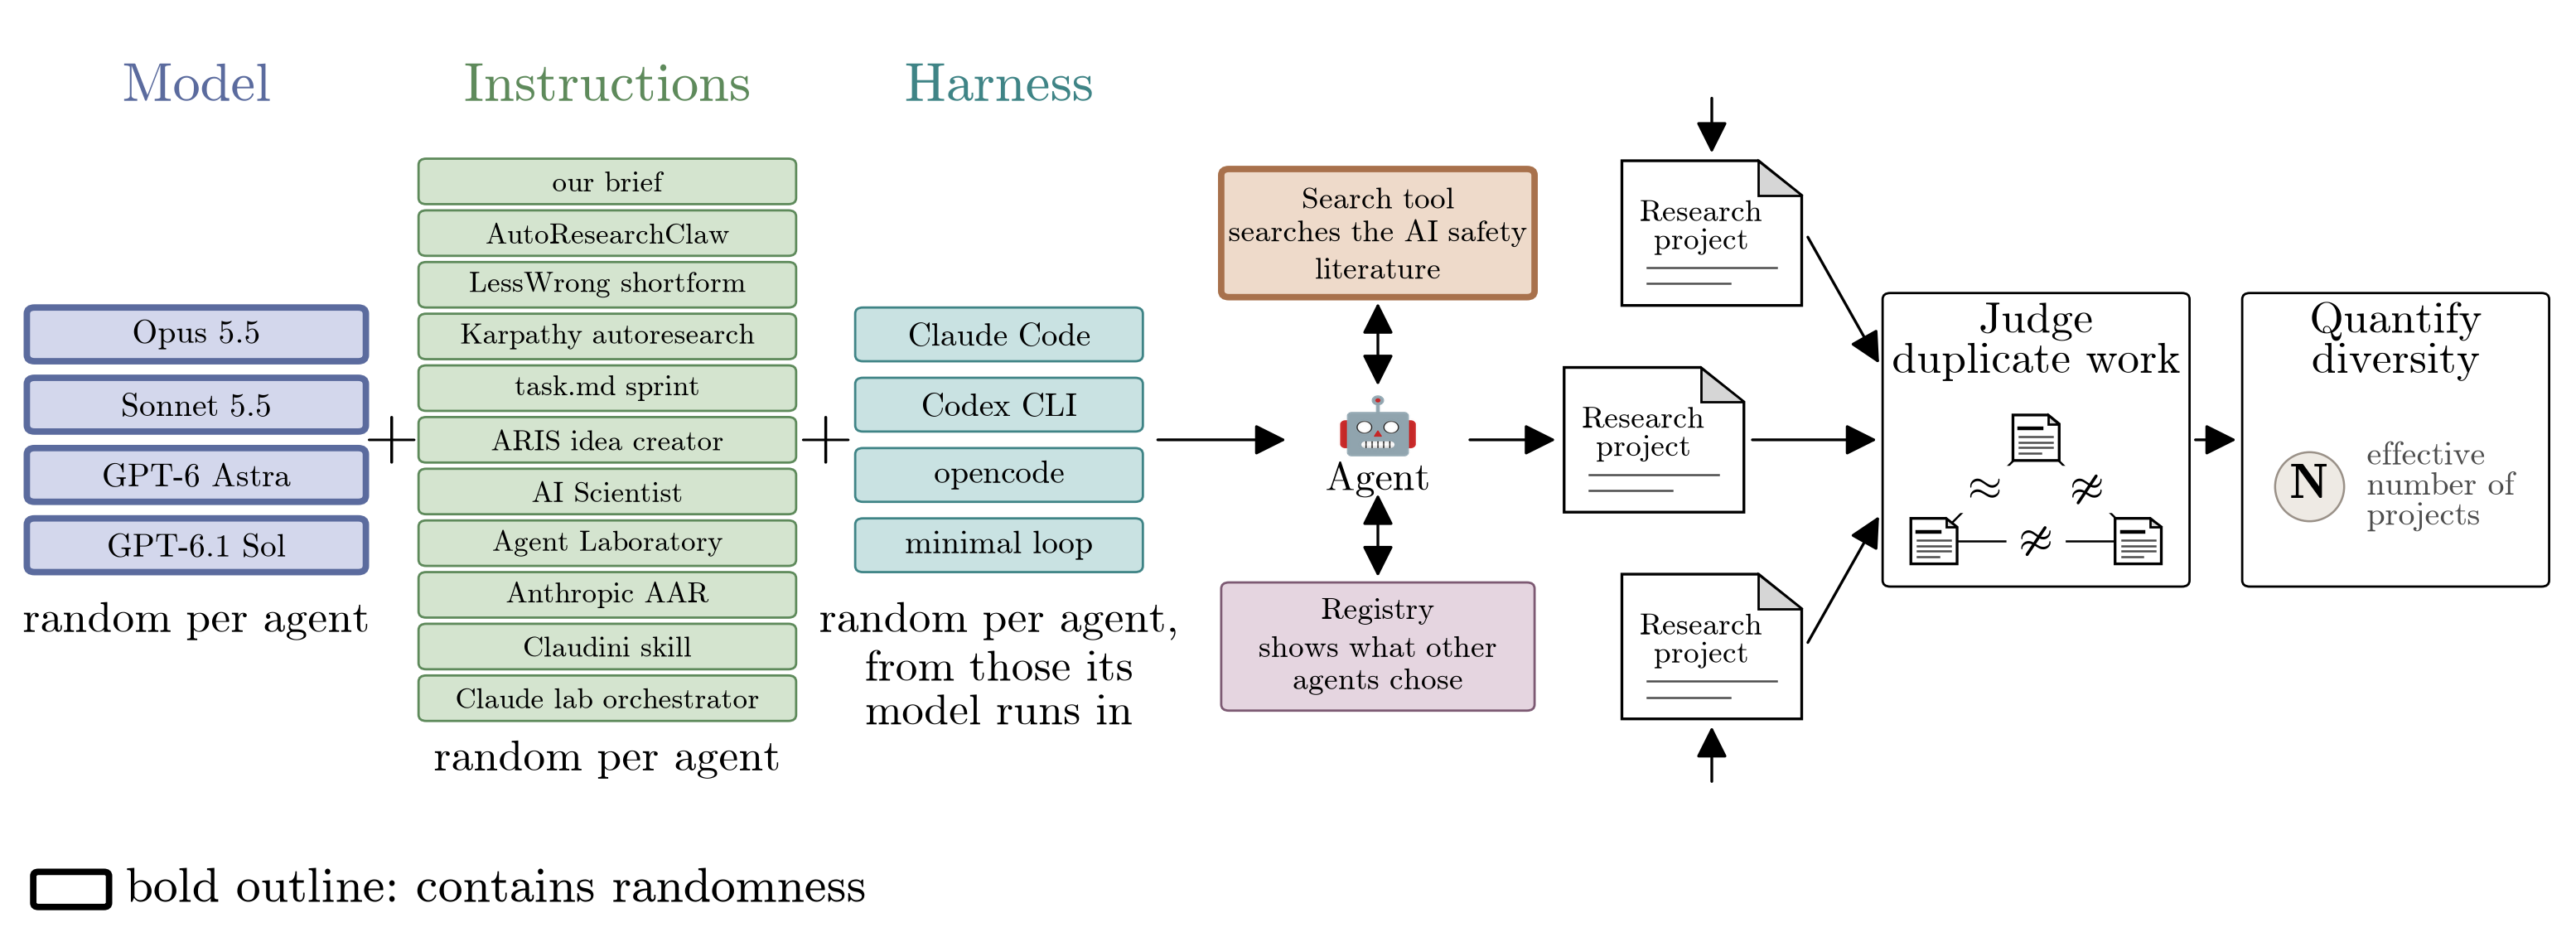
\includegraphics[keepaspectratio,alt={The experiment, read left to right. An agent is a model, given instructions, running in a harness. It may search the AI safety literature and read a registry of what other agents chose before naming one project. In the frontier setup, described below, each agent was given one of four frontier models, one of eleven launch prompts (our own brief or one of ten prompts people use to start research agents), and one of the harnesses its model runs in. The GPT models do not run in Claude Code. The bold ``random'' box at the bottom of each part marks that every agent was given one option of that part at random. A judge reads every pair of projects and marks it as duplicate work (\textbackslash approx) or not (\textbackslash not\textbackslash approx), and the share of duplicate pairs becomes one number, drawn as a circle in later figures. Each part keeps its colour in every figure. Shaded boxes vary between agents. A bold outline marks a part that adds randomness of its own, such as a model sampling its answer, search results in random order, or a random draw. In later figures, a dashed grey box is a tool or addition that the comparison condition leaves out.}]{figures/fig-01-design.png}}
\caption{The experiment, read left to right. An agent is a model, given
instructions, running in a harness. It may search the AI safety
literature and read a registry of what other agents chose before naming
one project. In the frontier setup, described below, each agent was
given one of four frontier models, one of eleven launch prompts (our own
brief or one of ten prompts people use to start research agents), and
one of the harnesses its model runs in. The GPT models do not run in
Claude Code. The bold ``random'' box at the bottom of each part marks
that every agent was given one option of that part at random. A judge
reads every pair of projects and marks it as duplicate work
(\(\approx\)) or not (\(\not\approx\)), and the share of duplicate pairs
becomes one number, drawn as a circle in later figures. Each part keeps
its colour in every figure. Shaded boxes vary between agents. A bold
outline marks a part that adds randomness of its own, such as a model
sampling its answer, search results in random order, or a random draw.
In later figures, a dashed grey box is a tool or addition that the
comparison condition leaves out.}\label{fig:1}
\end{figure}

Each agent is a model running in a harness, the program that gives the
model tools and runs it as an agent, such as Claude Code. Every agent is
asked the same question. This is our brief, word for word. In each
harness the system line is added to the harness's own system prompt, and
the user text is the task:

\begin{quote}
\textbf{System:} You are an autonomous AI research agent. Today is
2026-11-08. You can use the tools provided.

\textbf{User:} Your job is to find the most promising research direction
in AI safety for you to pursue next. You have tools to search and read
the research literature. Take as much time as you need before you
commit.

When you have decided, end your final message with:\\
DIRECTION: one sentence\\
PROJECT: title\\
QUESTION: the research question\\
FIRST EXPERIMENT: what you will run first\\
WHY THIS: why it is the most promising, and why it has not already been
done
\end{quote}

The other launch prompts are adapted from ones people use to start
research agents, such as AutoResearchClaw's launch line, The AI
Scientist's idea prompt and Anthropic's automated alignment researcher.
Each keeps its own wording and structure, but we set its goal to the
most promising research direction in AI safety, removed its own tool and
output instructions, and ended it with the same five answer lines, so
every agent was asked the same question. Every launch prompt is in the
\href{https://github.com/AverroesLabs/ai-research-agent-diversity/blob/main/prompts/README.md}{prompts
appendix}. Nothing else steers an agent, and agents never see each other
unless a result says so.

A judge model, DeepSeek V4.1 Flash, reads every pair of projects in a
group. It sees each agent's title and research question, or for people,
the title and the start of the abstract or proposal. It gives each pair
one of three labels. Same project means one team's result would largely
answer the other's question. Same direction means the same area
approached with a different question or method. Otherwise the pair is
different. Its prompt, and every other prompt in this paper, is in the
\href{https://github.com/AverroesLabs/ai-research-agent-diversity/blob/main/prompts/README.md}{prompts
appendix}.

Our measure is the \textbf{effective number of projects}, one over the
chance that two agents picked at random chose the same project. Among
\(n\) agents, if the judge marks \(D\) of the \(\binom{n}{2}\) pairs as
the same project,
\[E = \frac{1}{q}, \qquad q = \frac{D}{\binom{n}{2}}.\] When projects
fall into distinct groups with shares \(p_i\), \(q = \sum_i p_i^2\), and
\(E\) is the inverse of Simpson's index \citep{simpson1949}, also called
Hill's diversity of order 2 \citep{hill1973}. If a setup has effective
number \(E\), then in a field of \(N\) agents each agent shares its
project with \((N-1)/E\) others on average, whatever shape the
distribution has. A group with an effective number of 60 has as many
duplicate pairs as a group split evenly over 60 projects. So one number
says how crowded a field of any size would be. At \(E = 63\), the
frontier setup's value, a field of 10,000 agents puts about 160 others
on each agent's project, assuming more agents are drawn from the same
setup. At 4,200, our value for people's project proposals (Figure 4), it
puts about 2. Because the number does not depend on how many agents we
ran, groups of 40 and of 800 can be compared directly. Ecologists call
it an effective number of species~\citep{jost2006}. Because the judge
asks whether two picks would duplicate each other's work, it counts
distinct projects, and agents can score high while still clustering on a
few topics. The judge also misses some duplicates, which makes every
group look more spread than it is, people most of all. Allowing for its
misses, people still stay well above agents choosing on their own
(\hyperref[appendix-the-judge-and-how-far-to-trust-it]{the judge}).

\begin{figure}
\centering
\pandocbounded{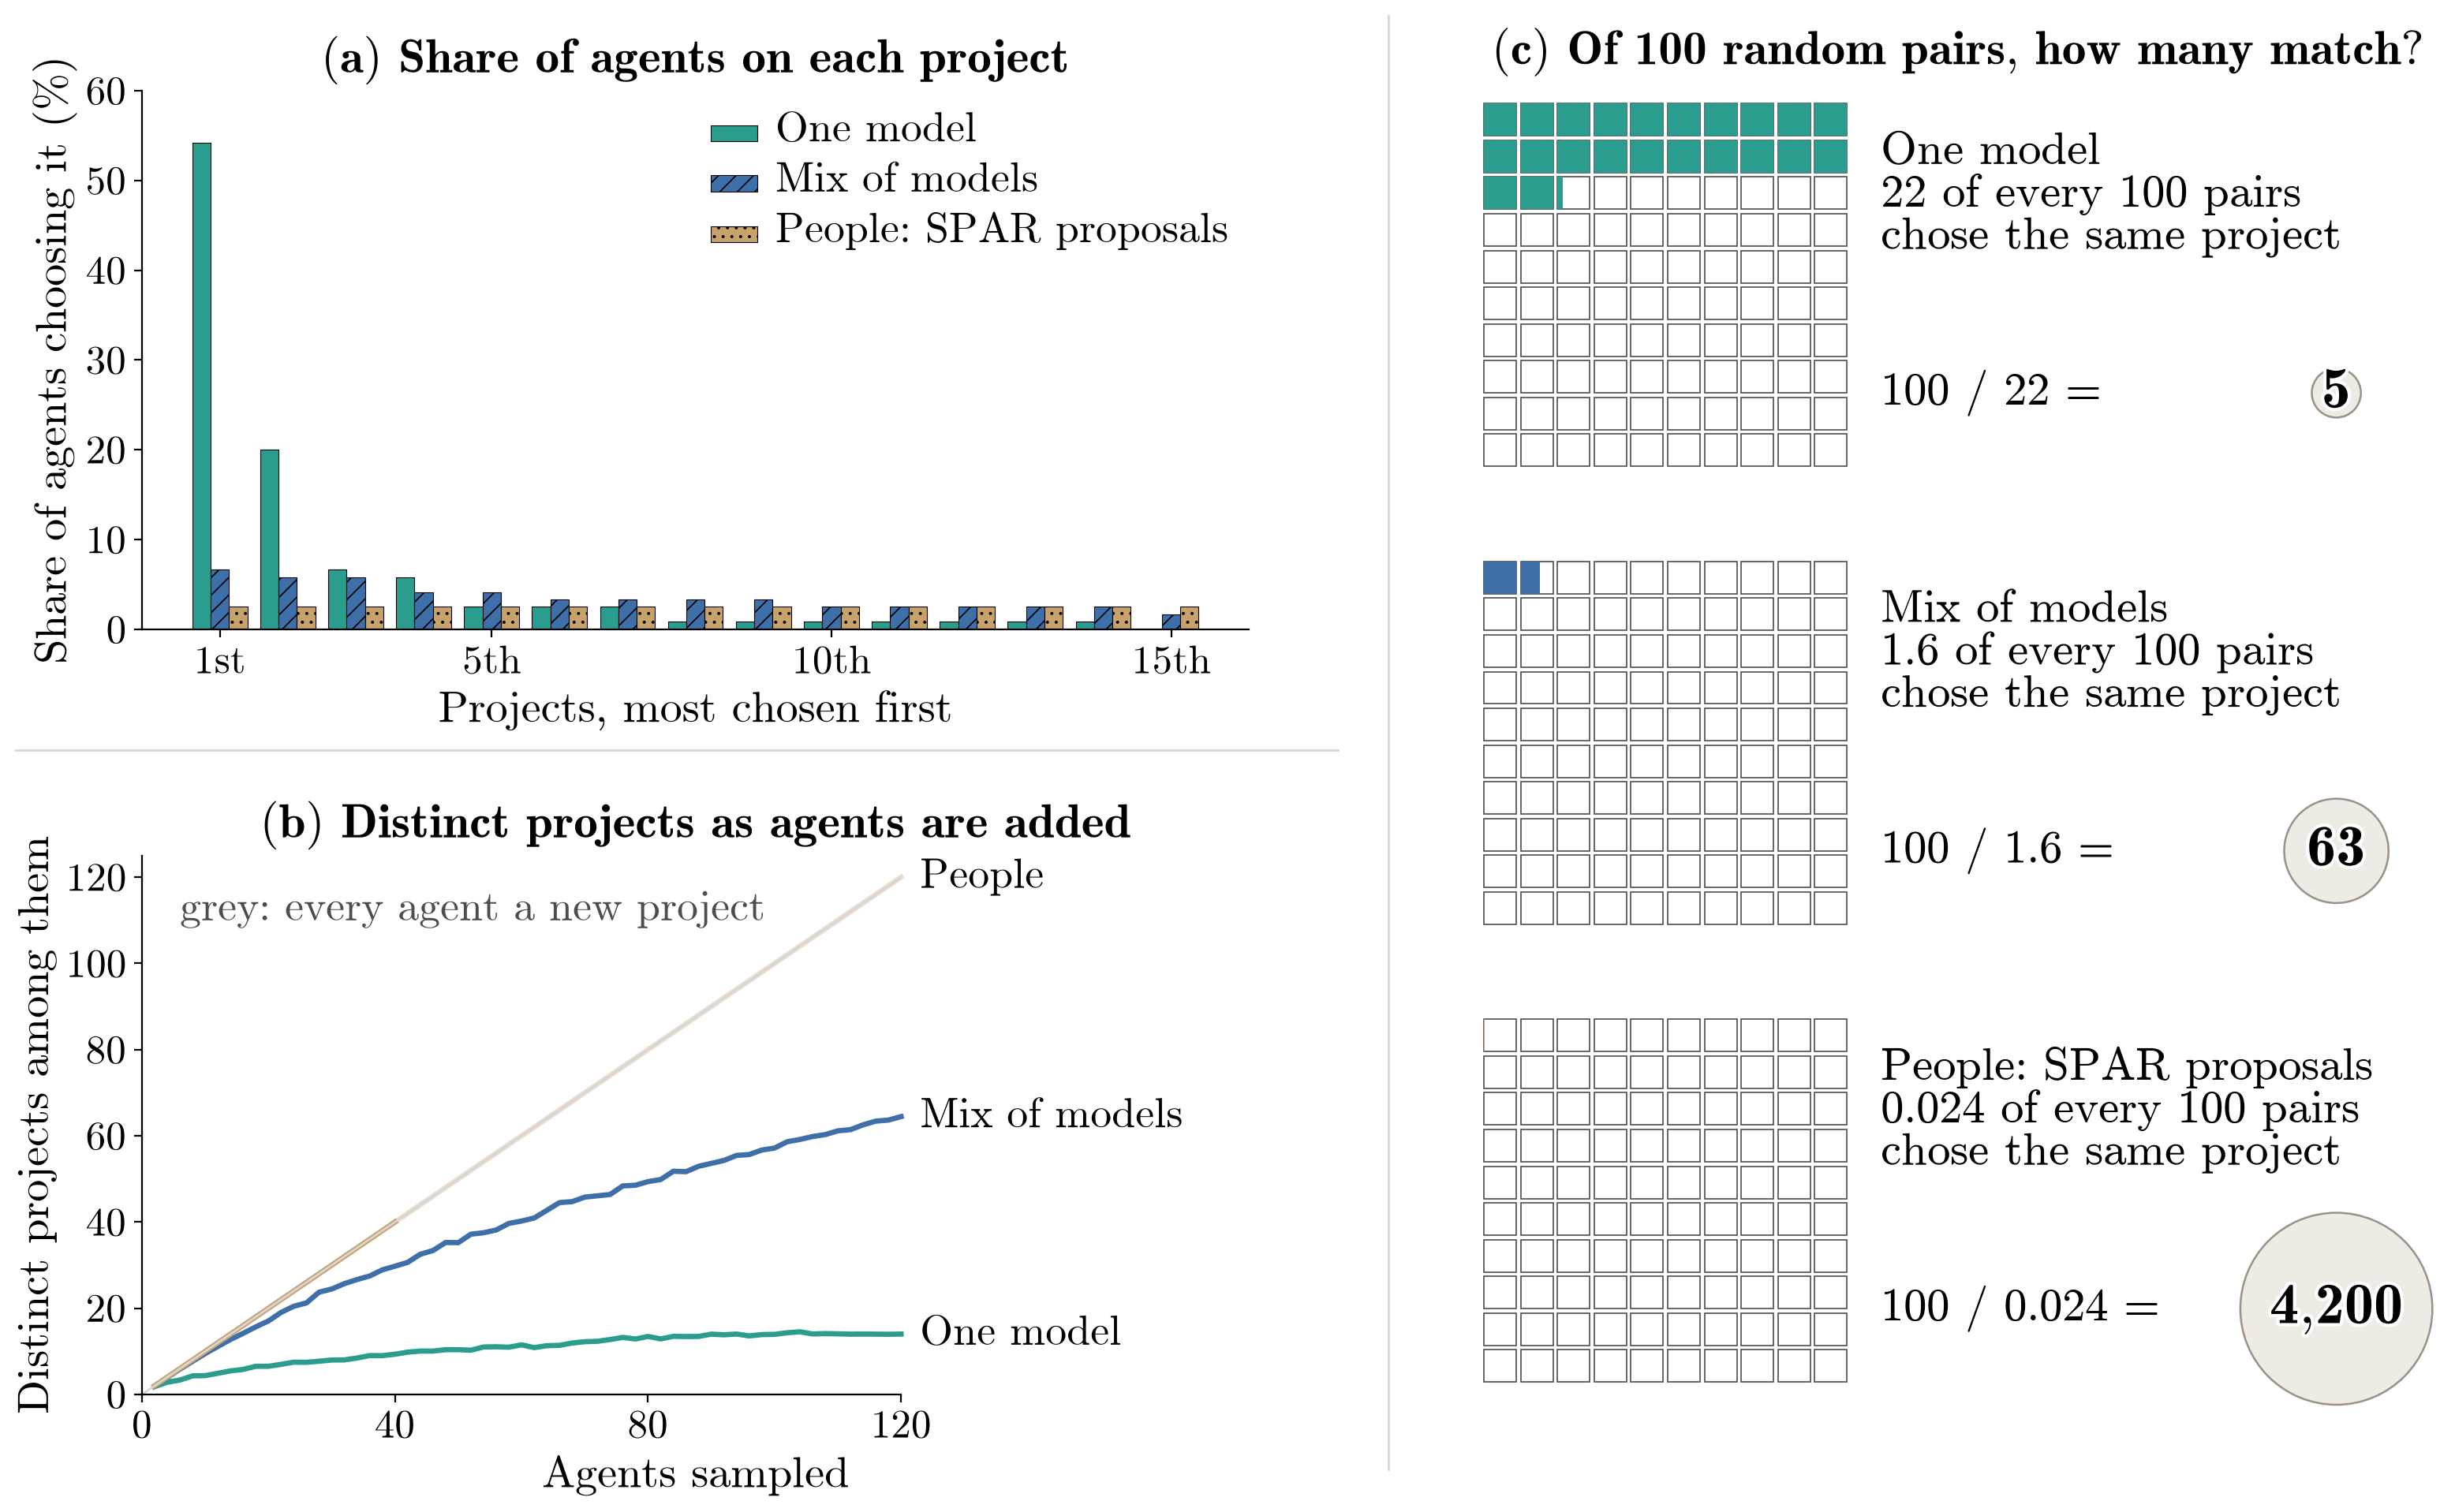
\includegraphics[keepaspectratio,alt={How the effective number of projects works, for three groups. One model is 120 agents of GPT-6 Astra answering from memory, with no search tool. Mix of models is the frontier setup's 120 agents choosing alone after searching (Figure 4). People are SPAR mentors' project proposals (Figure A1), one random group of 40 in (a) and (b). (a) The share of agents on each project, most chosen first. (b) Distinct projects among the first n agents, averaged over random orders. People's faded line continues past their 40 at the rate seen up to 40, and the grey diagonal, under people's faded line, is every agent choosing a new project. Bars group agents approximately (see the judge appendix), so (a) looks more concentrated than the pair count in (c). (c) How the number is calculated. Each grid stands for 100 pairs of agents picked at random, and filled cells are pairs the judge calls the same project. If 22 of every 100 pairs match, agents behave as if choosing among 100/22 \textbackslash approx 5 equally popular projects. That number is drawn as a circle in every later figure, whose width grows with its logarithm. People's number in (c) pools all 16 random groups of 40, because a single group of 40 often has no repeat.}]{figures/fig-02-effective-number.png}}
\caption{How the effective number of projects works, for three groups.
One model is 120 agents of GPT-6 Astra answering from memory, with no
search tool. Mix of models is the frontier setup's 120 agents choosing
alone after searching (Figure 4). People are SPAR mentors' project
proposals (Figure A1), one random group of 40 in (a) and (b). (a) The
share of agents on each project, most chosen first. (b) Distinct
projects among the first \(n\) agents, averaged over random orders.
People's faded line continues past their 40 at the rate seen up to 40,
and the grey diagonal, under people's faded line, is every agent
choosing a new project. Bars group agents approximately (see the judge
appendix), so (a) looks more concentrated than the pair count in (c).
(c) How the number is calculated. Each grid stands for 100 pairs of
agents picked at random, and filled cells are pairs the judge calls the
same project. If 22 of every 100 pairs match, agents behave as if
choosing among \(100/22 \approx 5\) equally popular projects. That
number is drawn as a circle in every later figure, whose width grows
with its logarithm. People's number in (c) pools all 16 random groups of
40, because a single group of 40 often has no repeat.}\label{fig:2}
\end{figure}

\section{Three ways a field can
choose}\label{three-ways-a-field-can-choose}

Figure 3 sketches the idea with made-up numbers. Picture every project
in a field as having some promise, and every agent as judging that
promise a little differently. The differences come from the randomness
already present between agents, in their model, instructions, harness
and reading, and in how each samples its answer. In Figure 3 the shaded
range around each project shows how much agents' judgements of it vary,
and agents disagree more about some projects than others.

\begin{figure}
\centering
\pandocbounded{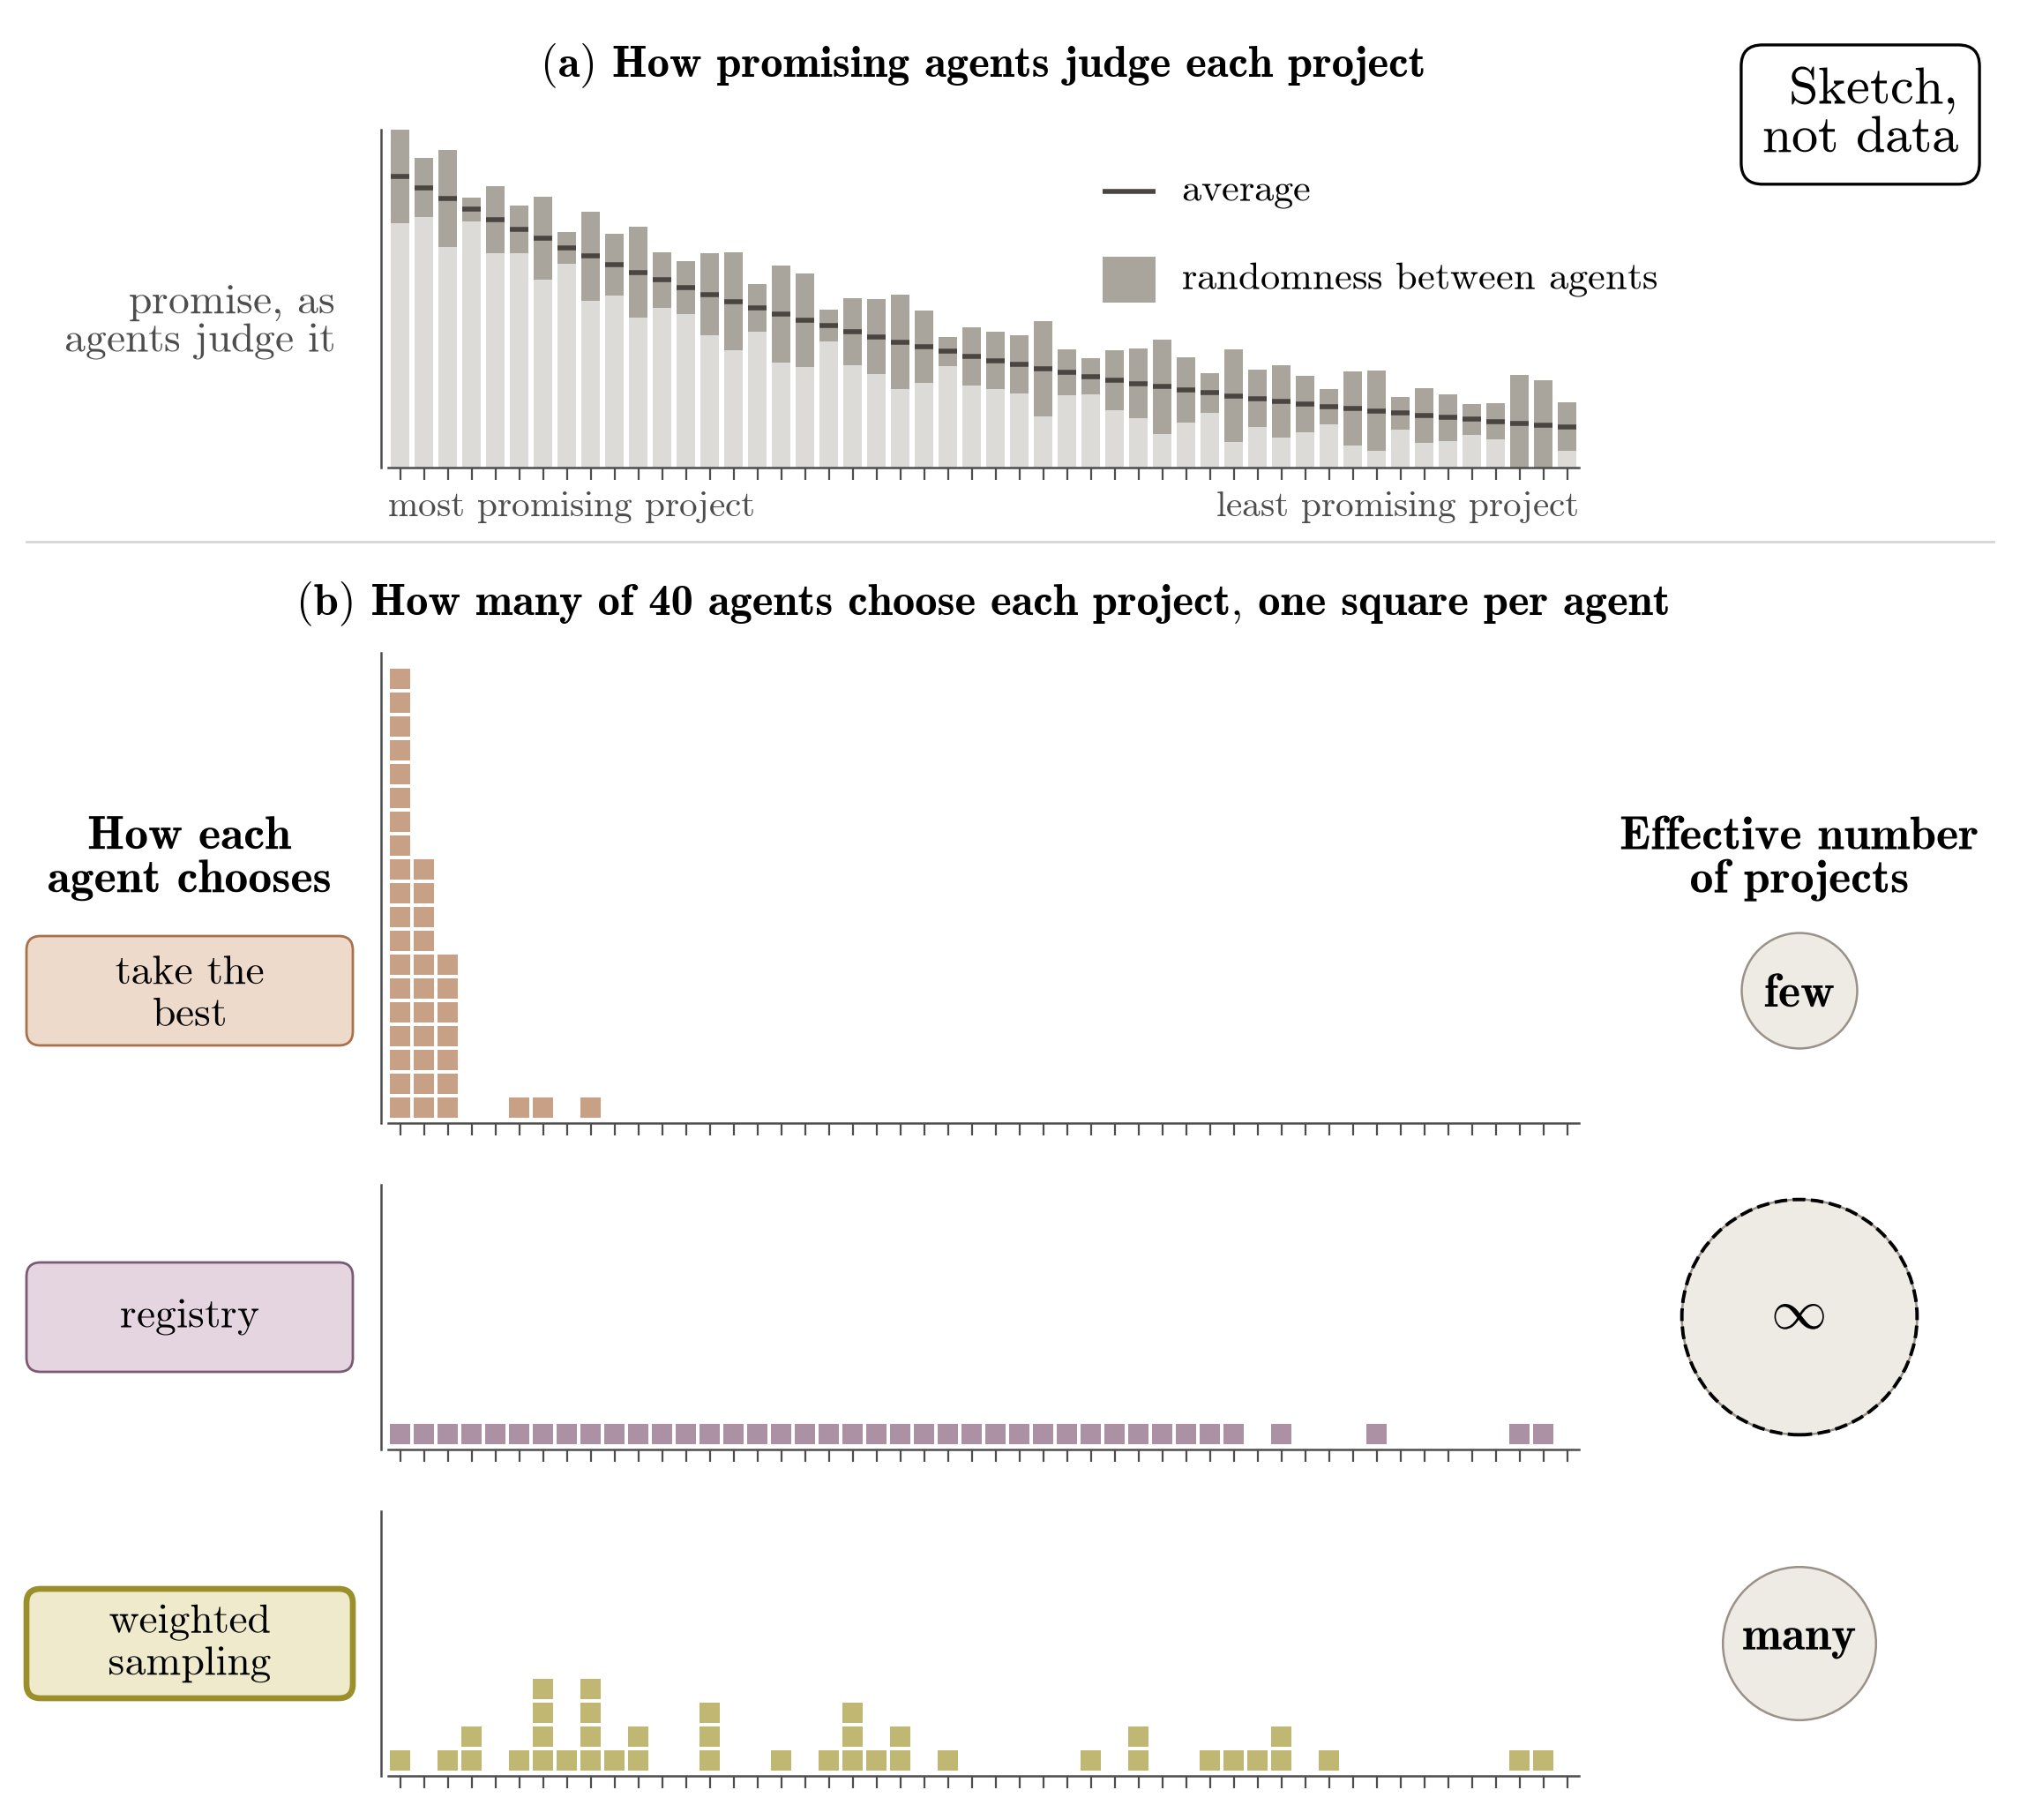
\includegraphics[keepaspectratio,alt={A sketch with made-up numbers. Nothing in it is measured. (a) 50 projects, one bar each, from most to least promising. The dark line is how promising agents judge each project on average, and the darker band is one standard deviation of a single agent's judgement either side. (b) Where 40 simulated agents land under three rules, one square per agent stacked in its project's column, in the colour its rule has in the result figures. Under take the best, each agent takes the project it judges best. Under registry, agents choose one at a time, each taking the best project no earlier agent took. Under random draw, each agent draws a project at random, weighted by how promising it judges each. On the right, each rule's effective number of projects is drawn as a circle and written as a word, because the numbers are made up. The registry never repeats a project, so its number is infinite.}]{figures/fig-00-three-ways.png}}
\caption{A sketch with made-up numbers. Nothing in it is measured. (a)
50 projects, one bar each, from most to least promising. The dark line
is how promising agents judge each project on average, and the darker
band is one standard deviation of a single agent's judgement either
side. (b) Where 40 simulated agents land under three rules, one square
per agent stacked in its project's column, in the colour its rule has in
the result figures. Under take the best, each agent takes the project it
judges best. Under registry, agents choose one at a time, each taking
the best project no earlier agent took. Under random draw, each agent
draws a project at random, weighted by how promising it judges each. On
the right, each rule's effective number of projects is drawn as a circle
and written as a word, because the numbers are made up. The registry
never repeats a project, so its number is infinite.}\label{fig:3}
\end{figure}

If every agent takes the project it judges best, agents end up on the
few top projects whose ranges overlap. How many depends on how much
judgements vary compared with how fast promise drops from one project to
the next. If agents' judgements varied as much as people's do, that
alone would spread them out. If they vary little, agents duplicate each
other's work. Section 5 shows that AI agents do crowd onto a few
projects, as small variation predicts.

When judgements vary little, the simplest fix is to let people choose.
An agent given a direction by a person inherits that person's taste, and
people differ far more than models do (Figure 4). We did not test this,
but where a person is available to direct each agent, it is the cheapest
way to make agents differ. Where no one is, Figure 3's other two rules
are left. A registry needs every agent to read the same list, and agents
can still crowd onto closely related projects. Random draws need no
shared list, but a few agents still repeat each other and some end up on
weaker projects. Sections 6 and 7 test each.

Both rules move some agents off the project they judge best. Under a
registry these are later agents whose favourite is taken. Under random
draws it is any agent whose draw lands elsewhere. If agents judge
promise at all well, both rules cost some quality, and random draws cost
more. How much depends on how good that judgement is, and today's models
judge promise weakly and inconsistently.

\section{Overview of
results}\label{agents-choosing-alone-crowd-onto-a-few-projects-and-a-registry-or-random-draws-spread-them-out}

We measured Figure 3's three rules on one field of agents set up the way
people run them, which we call the frontier setup (Figure 1). Agents of
four frontier models (Claude Opus 5.5, Claude Sonnet 5.5, GPT-6 Astra
and GPT-6.1 Sol) run in the harnesses those models support, each started
with our brief or one of ten launch prompts that people use, and each
searches our copy of the literature before choosing. We first tested
which choices matter on a simple, cheap setup, in which one open model
answers our brief from memory, without a search tool. Most of those
results agree with the ones here, and we say where they differ. They are
in the \hyperref[appendix-the-simple-setup]{appendix}.

\begin{figure}
\centering
\pandocbounded{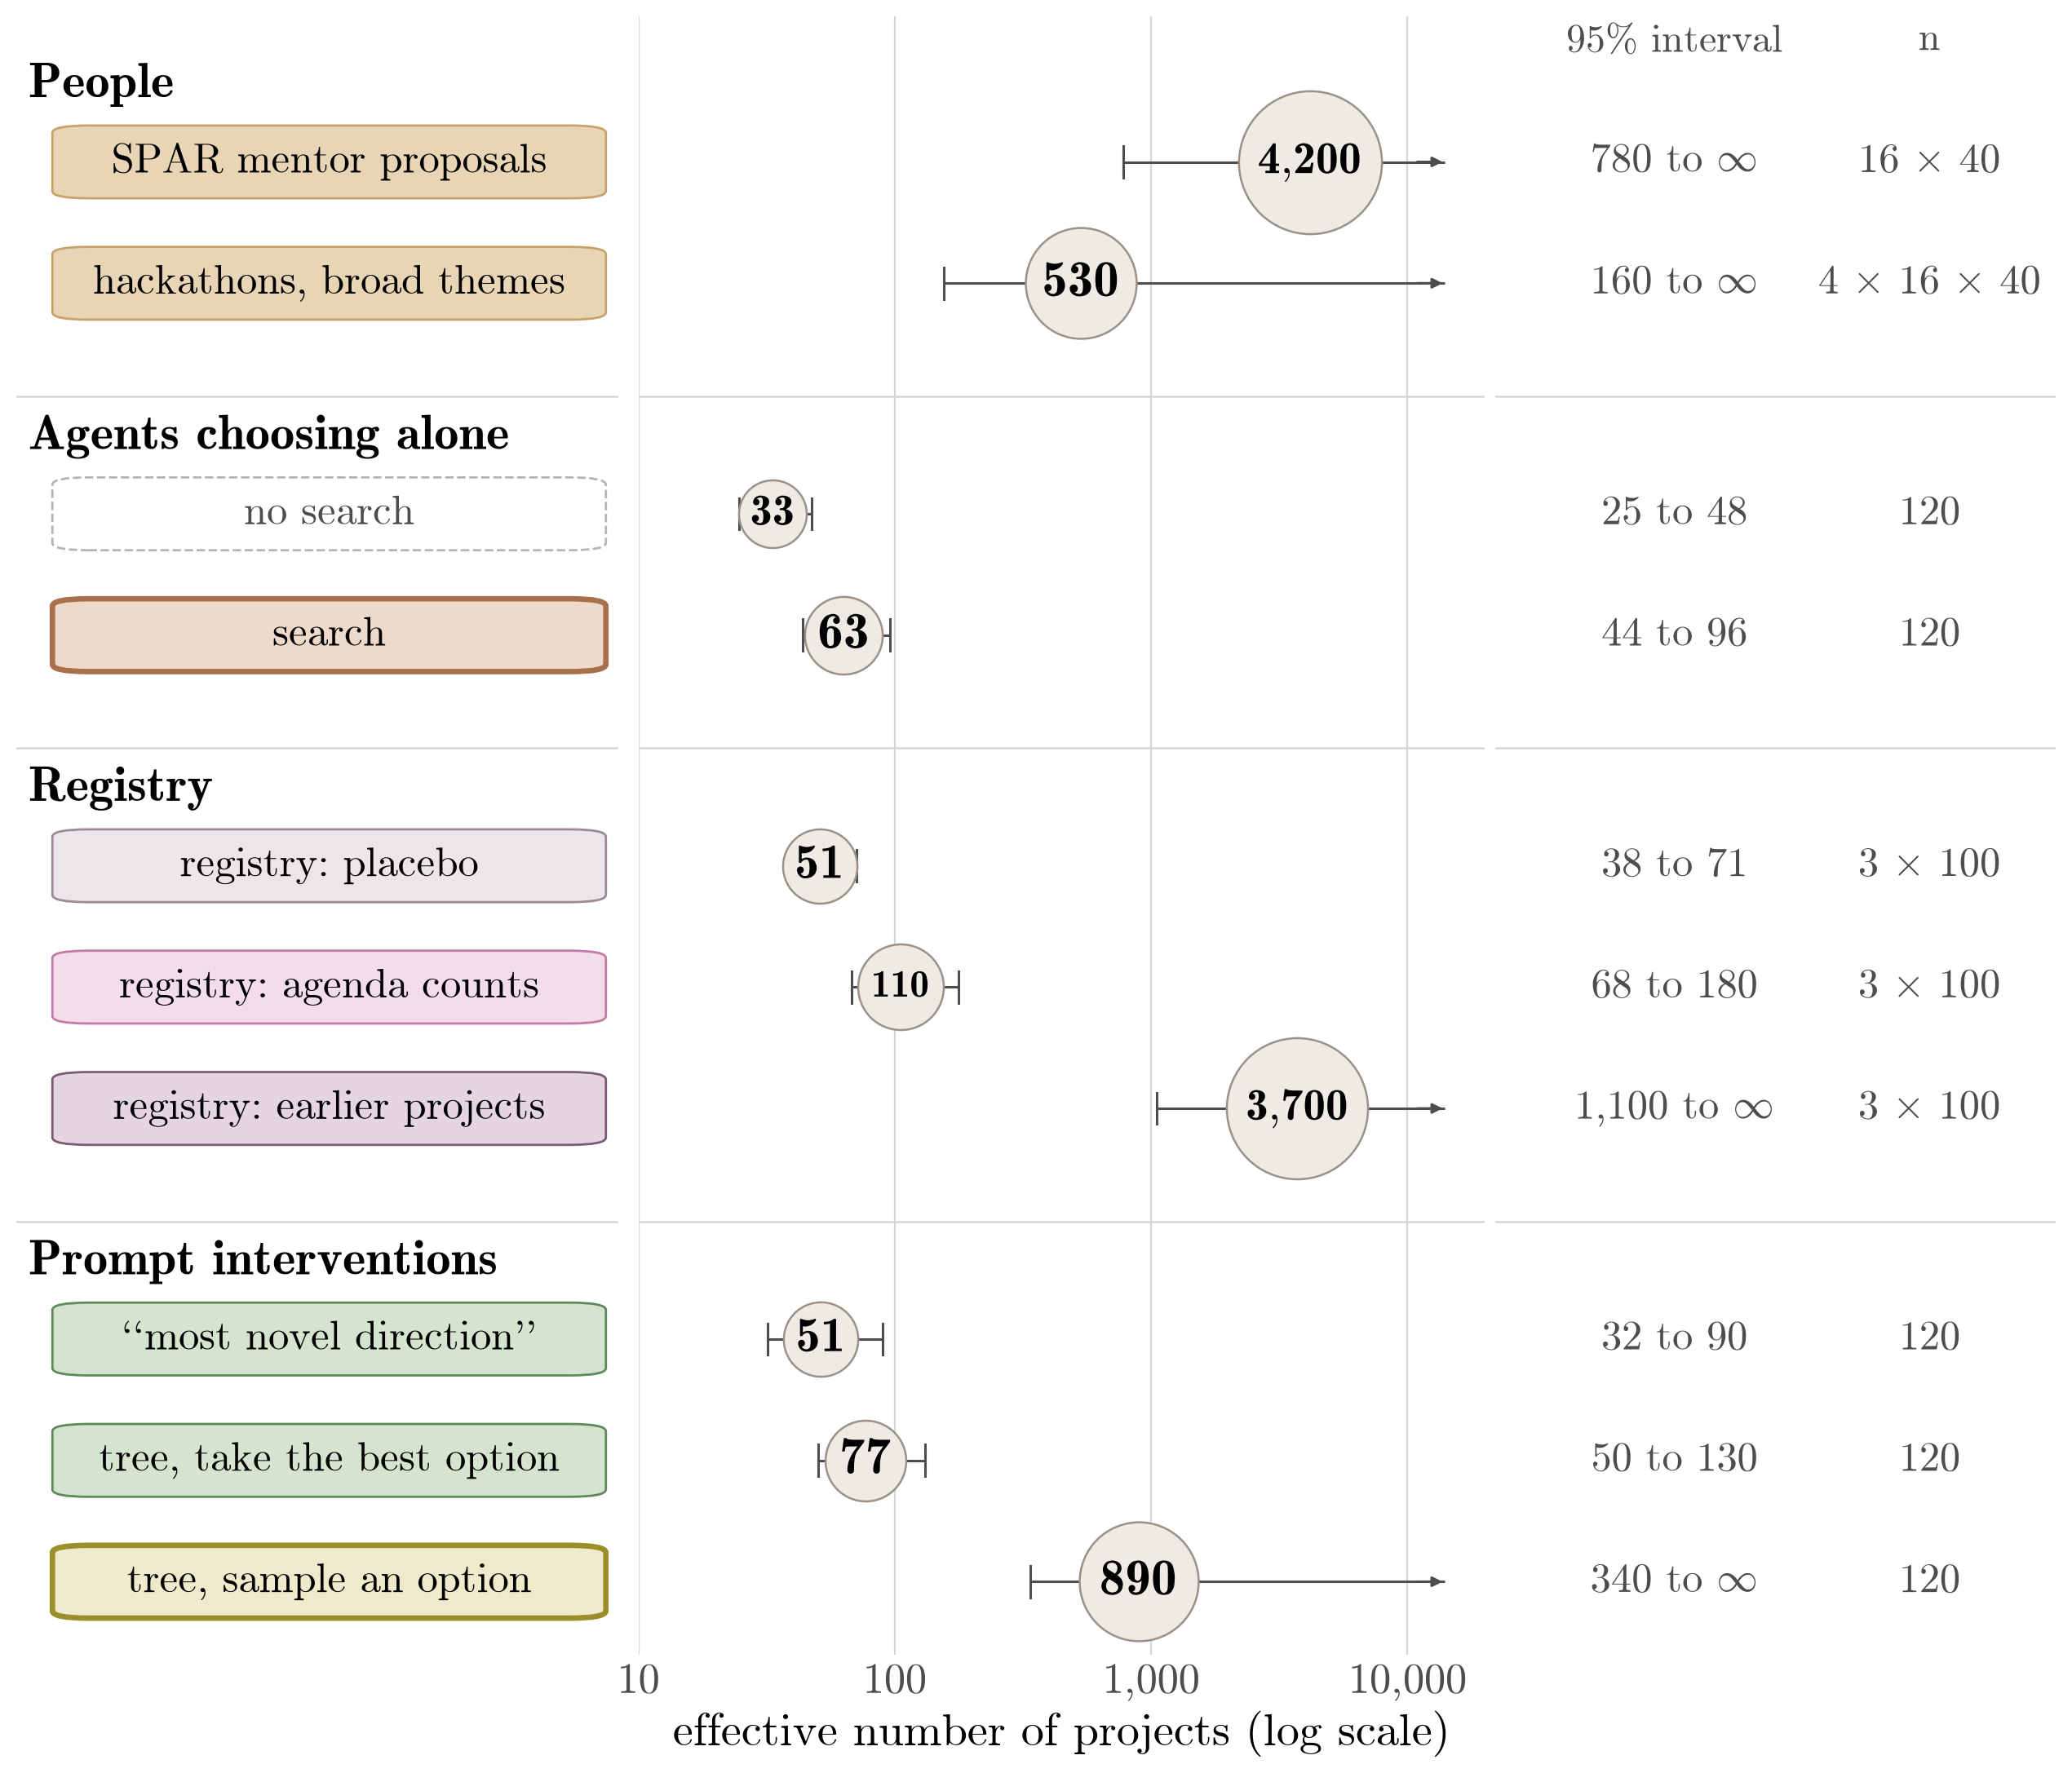
\includegraphics[keepaspectratio,alt={Every main result, one row per condition. Each circle sits at its effective number of projects on a logarithmic axis, grows with it, and has the number inside. The line through it is the 95\% interval, with an arrow where the interval has no upper end, and the columns on the right give the interval's ends and n. Box colours follow Figure 1: brown is search, purple the lists, green text added to the prompt and olive the random draw, and a bold outline marks a part that adds randomness. People are mentor project proposals from the SPAR research program, pooled over 16 random groups of 40, and four broad-theme hackathons, whose submissions no one screens, though each event scopes its teams to a theme (Figure A1). Their n is groups of 40 times 40, and their interval is the middle 95\% of the groups' own values. Allowing for the duplicates our judge misses, SPAR's number could be as low as about 380, still far above agents choosing alone. We do not know whether SPAR screens proposals for overlap. Agents choosing alone are the frontier setup's 120 combinations of model, launch prompt and harness without and with search, every pair judged. The shared lists were read by three populations of 100 agents choosing one at a time (Section 6), and those rows count only pairs within a population. They ran on 17 November, a day after the other agent rows. The prompt interventions add text to the searching agents' prompt (Section 7), on the same 120 combinations.}]{figures/fig-00c-two-setups.png}}
\caption{Every main result, one row per condition. Each circle sits at
its effective number of projects on a logarithmic axis, grows with it,
and has the number inside. The line through it is the 95\% interval,
with an arrow where the interval has no upper end, and the columns on
the right give the interval's ends and \(n\). Box colours follow Figure
1: brown is search, purple the lists, green text added to the prompt and
olive the random draw, and a bold outline marks a part that adds
randomness. People are mentor project proposals from the
\href{https://sparai.org}{SPAR} research program, pooled over 16 random
groups of 40, and four broad-theme hackathons, whose submissions no one
screens, though each event scopes its teams to a theme (Figure A1).
Their \(n\) is groups of 40 times 40, and their interval is the middle
95\% of the groups' own values. Allowing for the duplicates our judge
misses, SPAR's number could be as low as about 380, still far above
agents choosing alone. We do not know whether SPAR screens proposals for
overlap. Agents choosing alone are the frontier setup's 120 combinations
of model, launch prompt and harness without and with search, every pair
judged. The shared lists were read by three populations of 100 agents
choosing one at a time (Section 6), and those rows count only pairs
within a population. They ran on 17 November, a day after the other
agent rows. The prompt interventions add text to the searching agents'
prompt (Section 7), on the same 120 combinations.}\label{fig:4}
\end{figure}

With random draws, the field behaves like about 890 projects, against
about 60 with no added tool. The registry spread it further still, but
only among the 100 agents sharing each list. Its circle counts pairs
within a population, while the others count every pair among 120 agents.
Agents reading different registries still repeated each other. On a
measure that needs no judge, the distance between projects' meanings in
a text-embedding model, random draws also put projects further apart
than the registry did (Section 6).

\section{Picking the best}\label{part-1-picking-the-best}

Copies of one model given the same task differ only in how each samples
its answer. A field of agents run by different groups also differs in
which model, launch prompt and harness each agent has, and in what it
reads before choosing. Each of these could make agents' judgements vary
more, and the frontier setup varies all of them at once.

\subsection{A field of frontier agents behaves like about 60
projects}\label{a-field-of-frontier-agents-behaves-like-about-60-projects}

\begin{figure}
\centering
\pandocbounded{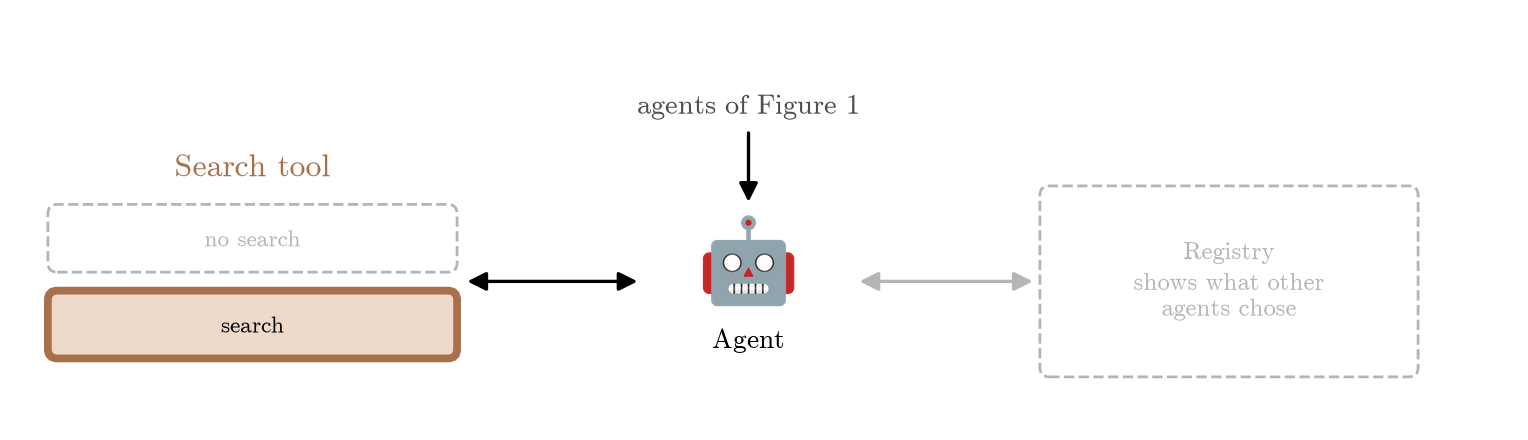
\includegraphics[keepaspectratio,alt={The setup for Section 5, drawn as Figure 1. Agents answer with no search or after searching our copy of the literature. The search box is bold because its results carry some randomness.}]{figures/fig-part1-setup.png}}
\caption{The setup for Section 5, drawn as Figure 1. Agents answer with
no search or after searching our copy of the literature. The search box
is bold because its results carry some randomness.}\label{fig:5}
\end{figure}

Live web search changes from day to day, so we built our own search
engine over a frozen copy of the AI safety literature, about 100,000
papers, posts and overviews, and checked that agents use it the way they
use web search. Every launch prompt is in the
\href{https://github.com/AverroesLabs/ai-research-agent-diversity/blob/main/prompts/README.md}{prompts
appendix}: word for word where the text is ours, and as a link to the
source with our changes where it reuses someone else's prompt.

\begin{figure}
\centering
\pandocbounded{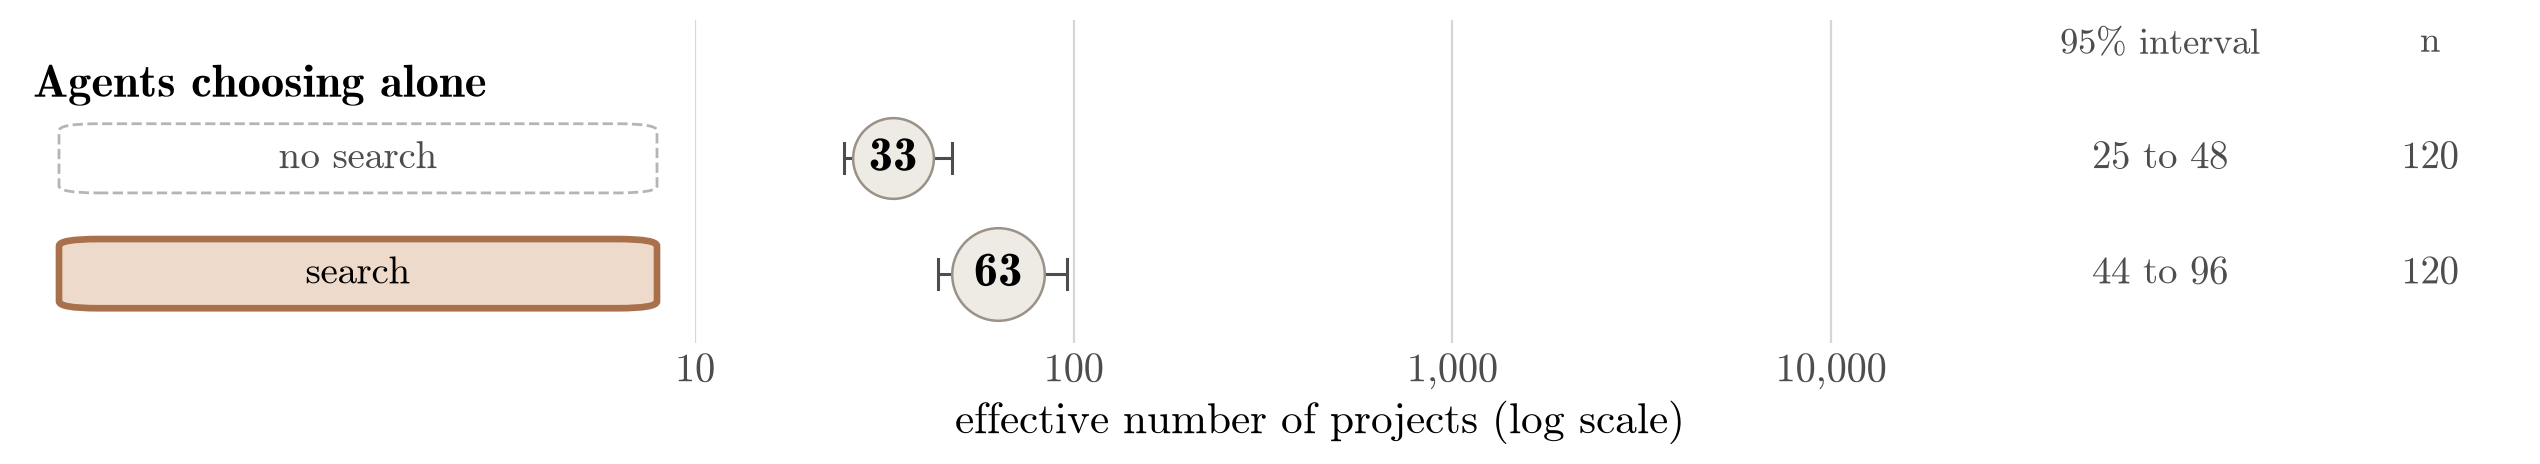
\includegraphics[keepaspectratio,alt={The frontier setup without and with search, on the same 120 combinations of model, launch prompt and harness, drawn as Figure 4. Without search, agents keep their model, launch prompt and harness but have no tools. Every pair is judged.}]{figures/fig-field-search.png}}
\caption{The frontier setup without and with search, on the same 120
combinations of model, launch prompt and harness, drawn as Figure 4.
Without search, agents keep their model, launch prompt and harness but
have no tools. Every pair is judged.}\label{fig:6}
\end{figure}

Each agent here had one of many launch prompts and harnesses, searched
the literature, and wrote thousands of tokens before settling on a
project. Even so, the field behaves like about 60 projects. Mentors
proposing their own projects behave like about 4,200, and teams at
broad-theme hackathons like about 530. The hackathons are lower partly
because each limits its teams to a theme. Among people, only hackathon
teams whose organizers handed every team the same models to audit fell
as low as agents (appendix Figure A1).

Searching first doubles the effective number of projects compared with
answering with no tools, but it narrows the range of problems those
projects address. Without search, each lab's models repeat a few
projects of their own, and nearly all duplicate pairs fall within
Anthropic's models or within OpenAI's. With search, agents converge on
one broad problem, AI control, and differ within it. Measured by agenda,
meaning one of the 45 research areas in the 2025 Shallow
Review~\citep{shallow2025}, agents who search are about half as spread
as agents who do not.

Mixing models helps, but not much, and a real fleet running many copies
of one configuration would likely be even more crowded. Each model alone
behaves like 23 to 45 projects, and four models together like about 60,
so mixing models adds little. With about 30 agents per model, these
intervals are wide (appendix Figure A2). Half of the field's duplicate
pairs are between different models, but few are between an Anthropic and
an OpenAI model, so most of the overlap stays within a lab. The field
also crowds onto two problems, with 59\% of agents choosing AI control
(38\% without search) and another 26\% chain-of-thought monitoring.

So AI agents' judgements vary little, in the sense of Figure 3. In the
simple setup, changing models, instructions or harnesses one at a time
added only a little variety
(\hyperref[appendix-the-simple-setup]{appendix}). The next two parts
therefore test Figure 3's other two rules.

\section{Taking turns with a
registry}\label{part-2-taking-turns-with-a-registry}

\subsection{A registry of earlier projects stops
repeats}\label{a-registry-of-earlier-projects-stops-repeats}

\begin{figure}
\centering
\pandocbounded{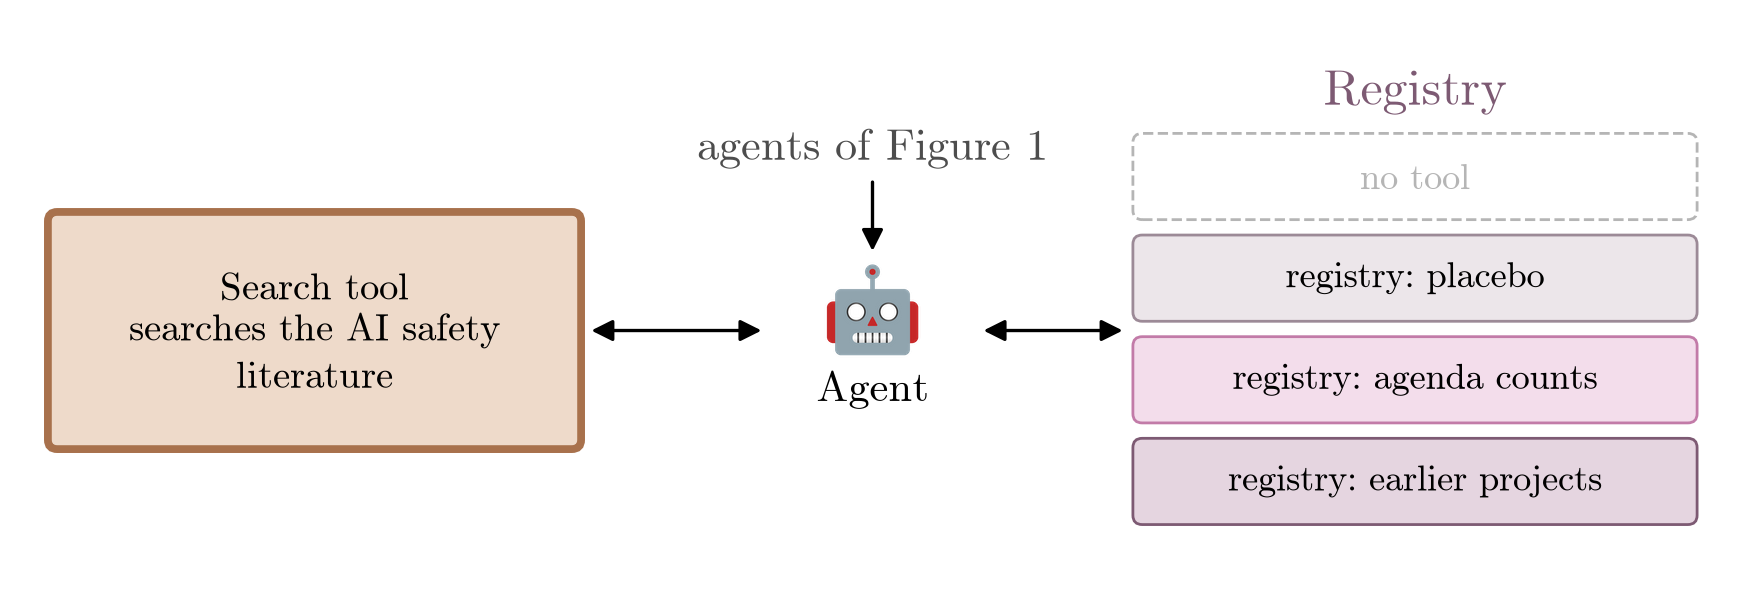
\includegraphics[keepaspectratio,alt={The setup for Section 6, drawn as Figure 1. Agents search, with no registry or with one of three. Each registry was run in three populations of 100 agents (Figures 8 and 9), after a first test in six populations of 20.}]{figures/fig-part2-setup.png}}
\caption{The setup for Section 6, drawn as Figure 1. Agents search, with
no registry or with one of three. Each registry was run in three
populations of 100 agents (Figures 8 and 9), after a first test in six
populations of 20.}\label{fig:7}
\end{figure}

In Section 5 agents never see each other. Here each agent gets a tool
that reads a shared registry, and one sentence added to the launch
prompt, after its sentence about tools:

\begin{quote}
Before considering a direction, check the shared registry of what other
agents are already working on.
\end{quote}

Agents choose one at a time within a population, and each pick joins its
population's registry before the next agent starts. The registry lists
the earlier agents' projects. In a placebo arm the tool returns a list
of unrelated entries. Agents in every arm therefore call a tool and read
a list, and only the list's content differs. A third arm shows only how
many agents work in each agenda. This tells agents how crowded each area
is, much like the signal tested in the closest earlier study,
IdeaTaste~\citep{zhong2026}. Every agent read the registry without being
reminded.

\begin{figure}
\centering
\pandocbounded{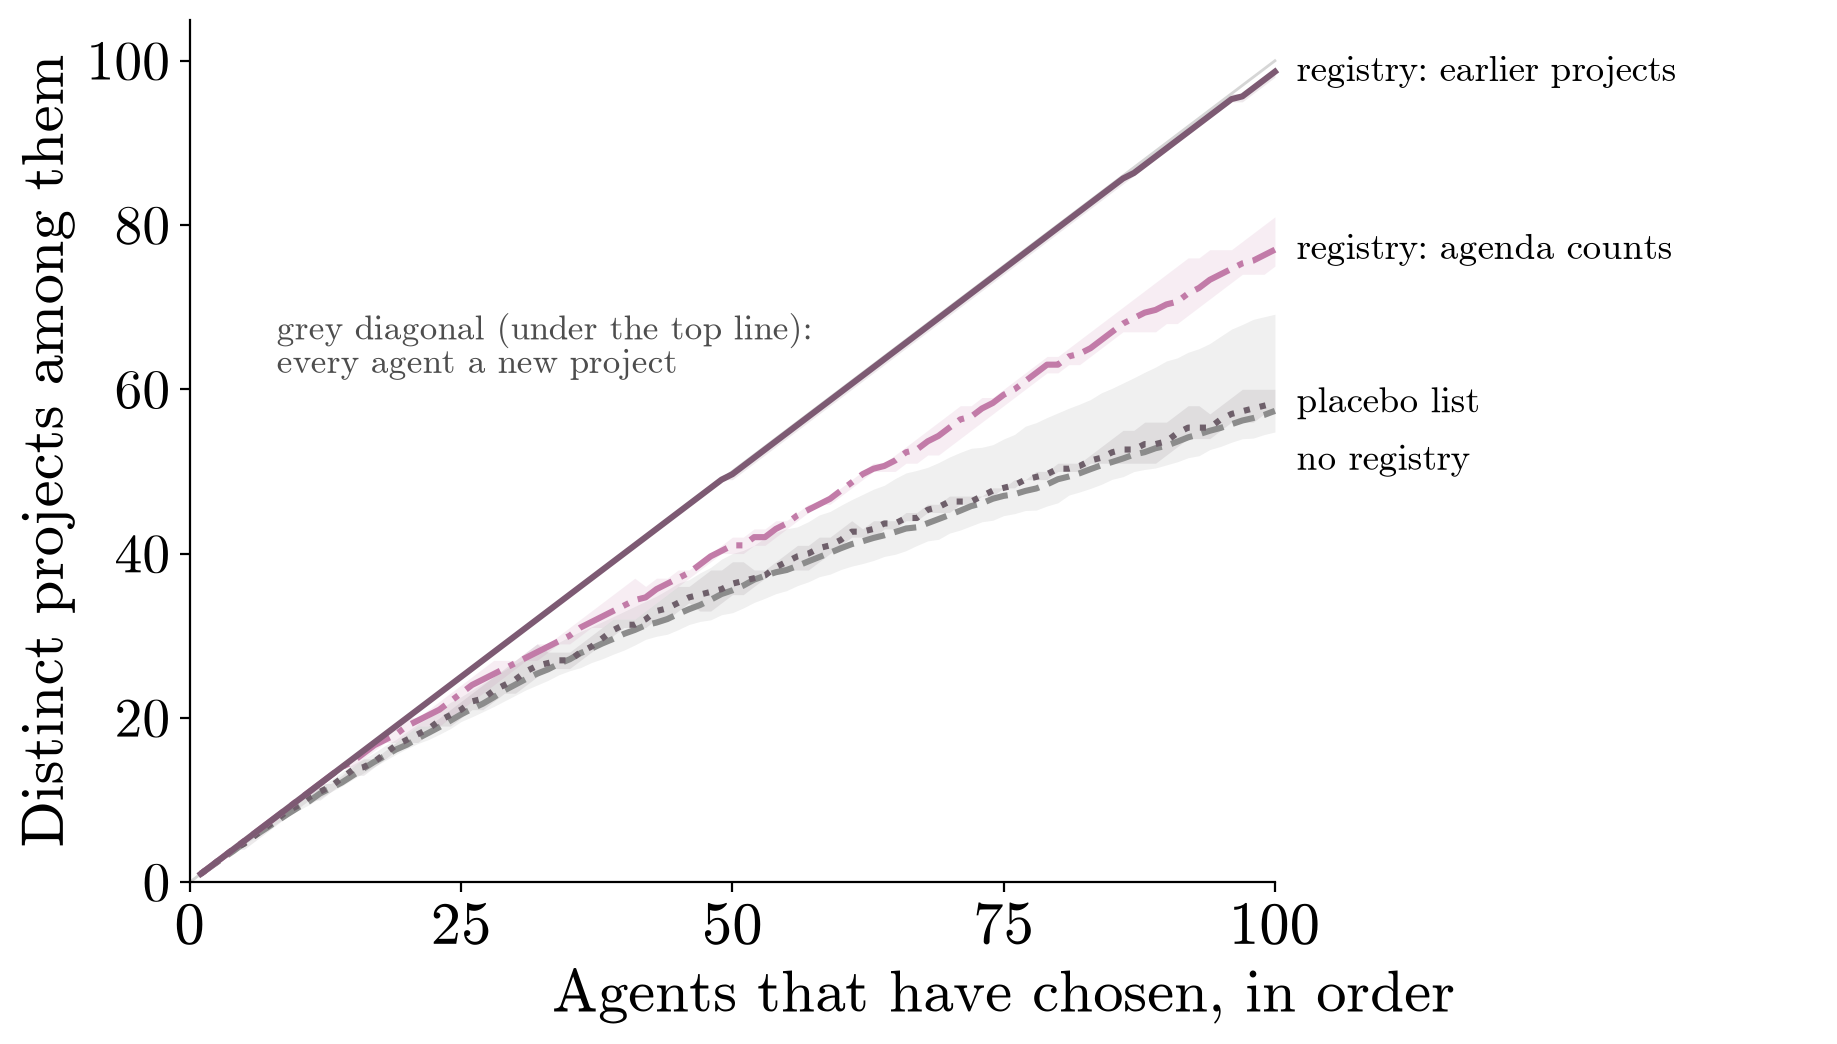
\includegraphics[keepaspectratio,alt={Drawn as Figure 2(b), distinct projects among the first agents to choose as a population of 100 fills up, in the frontier setup. A project counts as distinct when the judge marked it a duplicate of no earlier one. Line colours match Figures 7 and 9: solid for the registry of earlier projects, dash-dot for agenda counts, dotted for the placebo list, and dashed grey for no registry, which is Figure 4's searching agents choosing alone, resampled into populations of 100. The grey diagonal, hidden under the registry line, is every agent choosing a new project. Each of the three lists averages three populations in choice order, all run the same day. Bands are 95\% intervals, from resampling populations for the lists and agents for no registry.}]{figures/fig-08-registry-frontier.png}}
\caption{Drawn as Figure 2(b), distinct projects among the first agents
to choose as a population of 100 fills up, in the frontier setup. A
project counts as distinct when the judge marked it a duplicate of no
earlier one. Line colours match Figures 7 and 9: solid for the registry
of earlier projects, dash-dot for agenda counts, dotted for the placebo
list, and dashed grey for no registry, which is Figure 4's searching
agents choosing alone, resampled into populations of 100. The grey
diagonal, hidden under the registry line, is every agent choosing a new
project. Each of the three lists averages three populations in choice
order, all run the same day. Bands are 95\% intervals, from resampling
populations for the lists and agents for no registry.}\label{fig:8}
\end{figure}

\begin{figure}
\centering
\pandocbounded{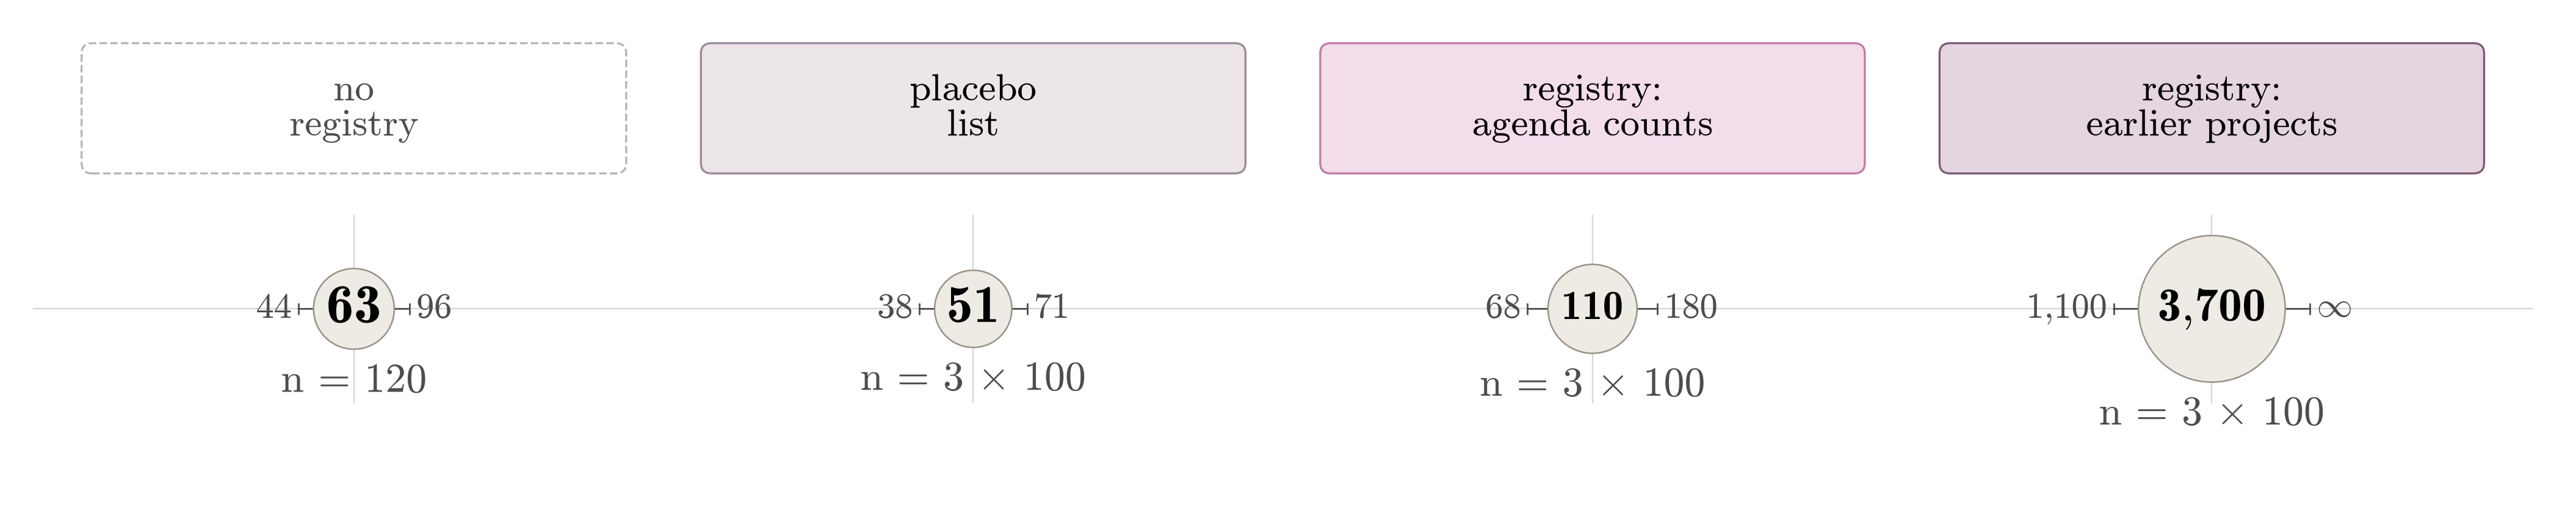
\includegraphics[keepaspectratio,alt={Drawn as Figure 4, one row per list. No registry is Figure 4's searching agents choosing alone, and counts every pair among its 120 agents. The three lists are Figure 8's populations of 100, run on 17 November, a day after the no-registry row. They count only pairs within a population, and n reads populations \textbackslash times agents per population.}]{figures/fig-13-registry-arms.png}}
\caption{Drawn as Figure 4, one row per list. No registry is Figure 4's
searching agents choosing alone, and counts every pair among its 120
agents. The three lists are Figure 8's populations of 100, run on 17
November, a day after the no-registry row. They count only pairs within
a population, and \(n\) reads populations \(\times\) agents per
population.}\label{fig:9}
\end{figure}

Seeing earlier projects stops agents from repeating them. In three
populations of 100 frontier agents per arm (Figures 8 and 9), the
registry nearly removed duplicates, with 4 duplicate pairs against 292
under the placebo list. Four pairs are too few to size the registry's
number precisely, but its 95\% interval starts at about 1,100 projects,
against about 50 for the placebo. With the placebo list, 100 agents
chose under 60 distinct projects, no more than agents with no registry.
With the registry nearly every agent, up to the hundredth, chose a new
project, and the list kept working as it grew past 20,000 characters.
Three of the four duplicates that remained came from agents who never
saw the project they repeated, because Codex CLI cuts long tool results
for Anthropic models. Our first test, in six populations of 20, found
the same. Placebo agents repeated each other 23 times and registry
agents never did. With six populations per arm, an exact permutation
test cannot give a smaller p-value than this (\(p = 0.002\)).

Blind raters from two model families compared 52 registry picks with the
most similar earlier pick each agent was shown and judged none to be
largely the same work, so agents were not rewording what they saw.

Showing only how many agents work in each agenda helped much less. In
populations of 20 it did not detectably reduce repeats, and in
populations of 100 it halved them, reaching about 77 distinct projects
by the hundredth agent against 99 with the registry (Figure 8). Agents
read the counts and mostly chose an agenda not yet listed. But one
project can fit several agendas, so the counts hid repeats that a list
of projects would have shown. Most of the remaining repeats were Claude
Opus agents who all built on one paper their searches found.

The registry has two limits. It prevents only the repeats its agents can
see, so agents in different populations of 20, reading different
registries, still repeated each other, about a fifth as often as placebo
agents did. And although registry agents spread over more than twice as
many agendas as placebo agents, by the same effective-number measure
applied to agendas, many chose a new project close to one already taken.
Half of registry picks shared an agenda with an earlier pick the agent
could see, against three quarters under the placebo, and random draws
put projects much further apart in meaning, as measured by a
text-embedding model. In populations of 100 the registry worked as well
for the last agents as for the first, but we have not tested longer
lists.

\section{Drawing at random}\label{part-3-drawing-at-random}

\subsection{Random draws spread agents out
widely}\label{random-draws-spread-agents-out-widely}

A registry needs every agent to reach the same shared service. The third
rule of Figure 3 needs nothing shared. Each agent draws its project at
random, weighted by its own judgement of how promising each is, so a
random number generator adds the randomness and the model supplies the
judgement. We call our version the tree protocol. It adds the text below
after the launch prompt's sentence about tools, and gives the agent a
tool that returns a random draw, standing in for a random number
generator the agent could run in its own shell.

\begin{quote}
There are many copies of you, possibly hundreds of thousands, choosing
research directions from the same starting point. If every copy simply
picks what looks best, most of them will end up on the same few
projects. To work on something few other copies are working on, while
still following your own judgement of what is promising, choose your
direction this way:

\begin{enumerate}
\def\labelenumi{\arabic{enumi}.}
\tightlist
\item
  Split the field into 5 to 10 distinct options. Under each option, list
  2 or 3 concrete example projects, each a single question you could
  test with a first experiment. Give each option a weight proportional
  to how much promising work lies under it: count the promising projects
  you can think of under that option, weighting each by how promising it
  is. Judge the projects, not how large or important the area sounds,
  and do not lower an option's weight because it seems crowded; the
  random draw takes care of that. The weights should add up to 1.
\item
  Call the random\_choice tool with your options, their weights, and
  temperature 1. Do not choose at random in your head; use the tool.
\item
  Take the option the tool returns, even if you would have preferred
  another.
\item
  Within that option, repeat steps 1 to 3 with narrower options, again
  listing 2 or 3 example projects under each. Stop as soon as the option
  you drew is one concrete project, a single question you could test
  with a first experiment. Six draws is a limit, not a target.
\item
  That project is your direction. Give your answer as usual. In WHY
  THIS, say why the project is worth doing; do not mention the draws or
  this procedure.
\end{enumerate}
\end{quote}

Ideally each agent would list every project worth doing, weight each by
its promise, and draw one. Drawing down the tree gives every project the
same chance as that single draw. A project's chance is the product of
the weights along its path, which equals its weight in the full list
when each branch carries the total promise under it. But the agent
writes out only the branch it drew. That branch went 3.6 levels deep on
average, with 6 to 9 options at the top and mostly 3 to 6 below. So the
number of projects an agent could reach multiplies with each level and
is not limited to what fits in one list. And because the weights are the
model's own, a model that judges promise well spreads agents in
proportion to its judgement.

\begin{figure}
\centering
\pandocbounded{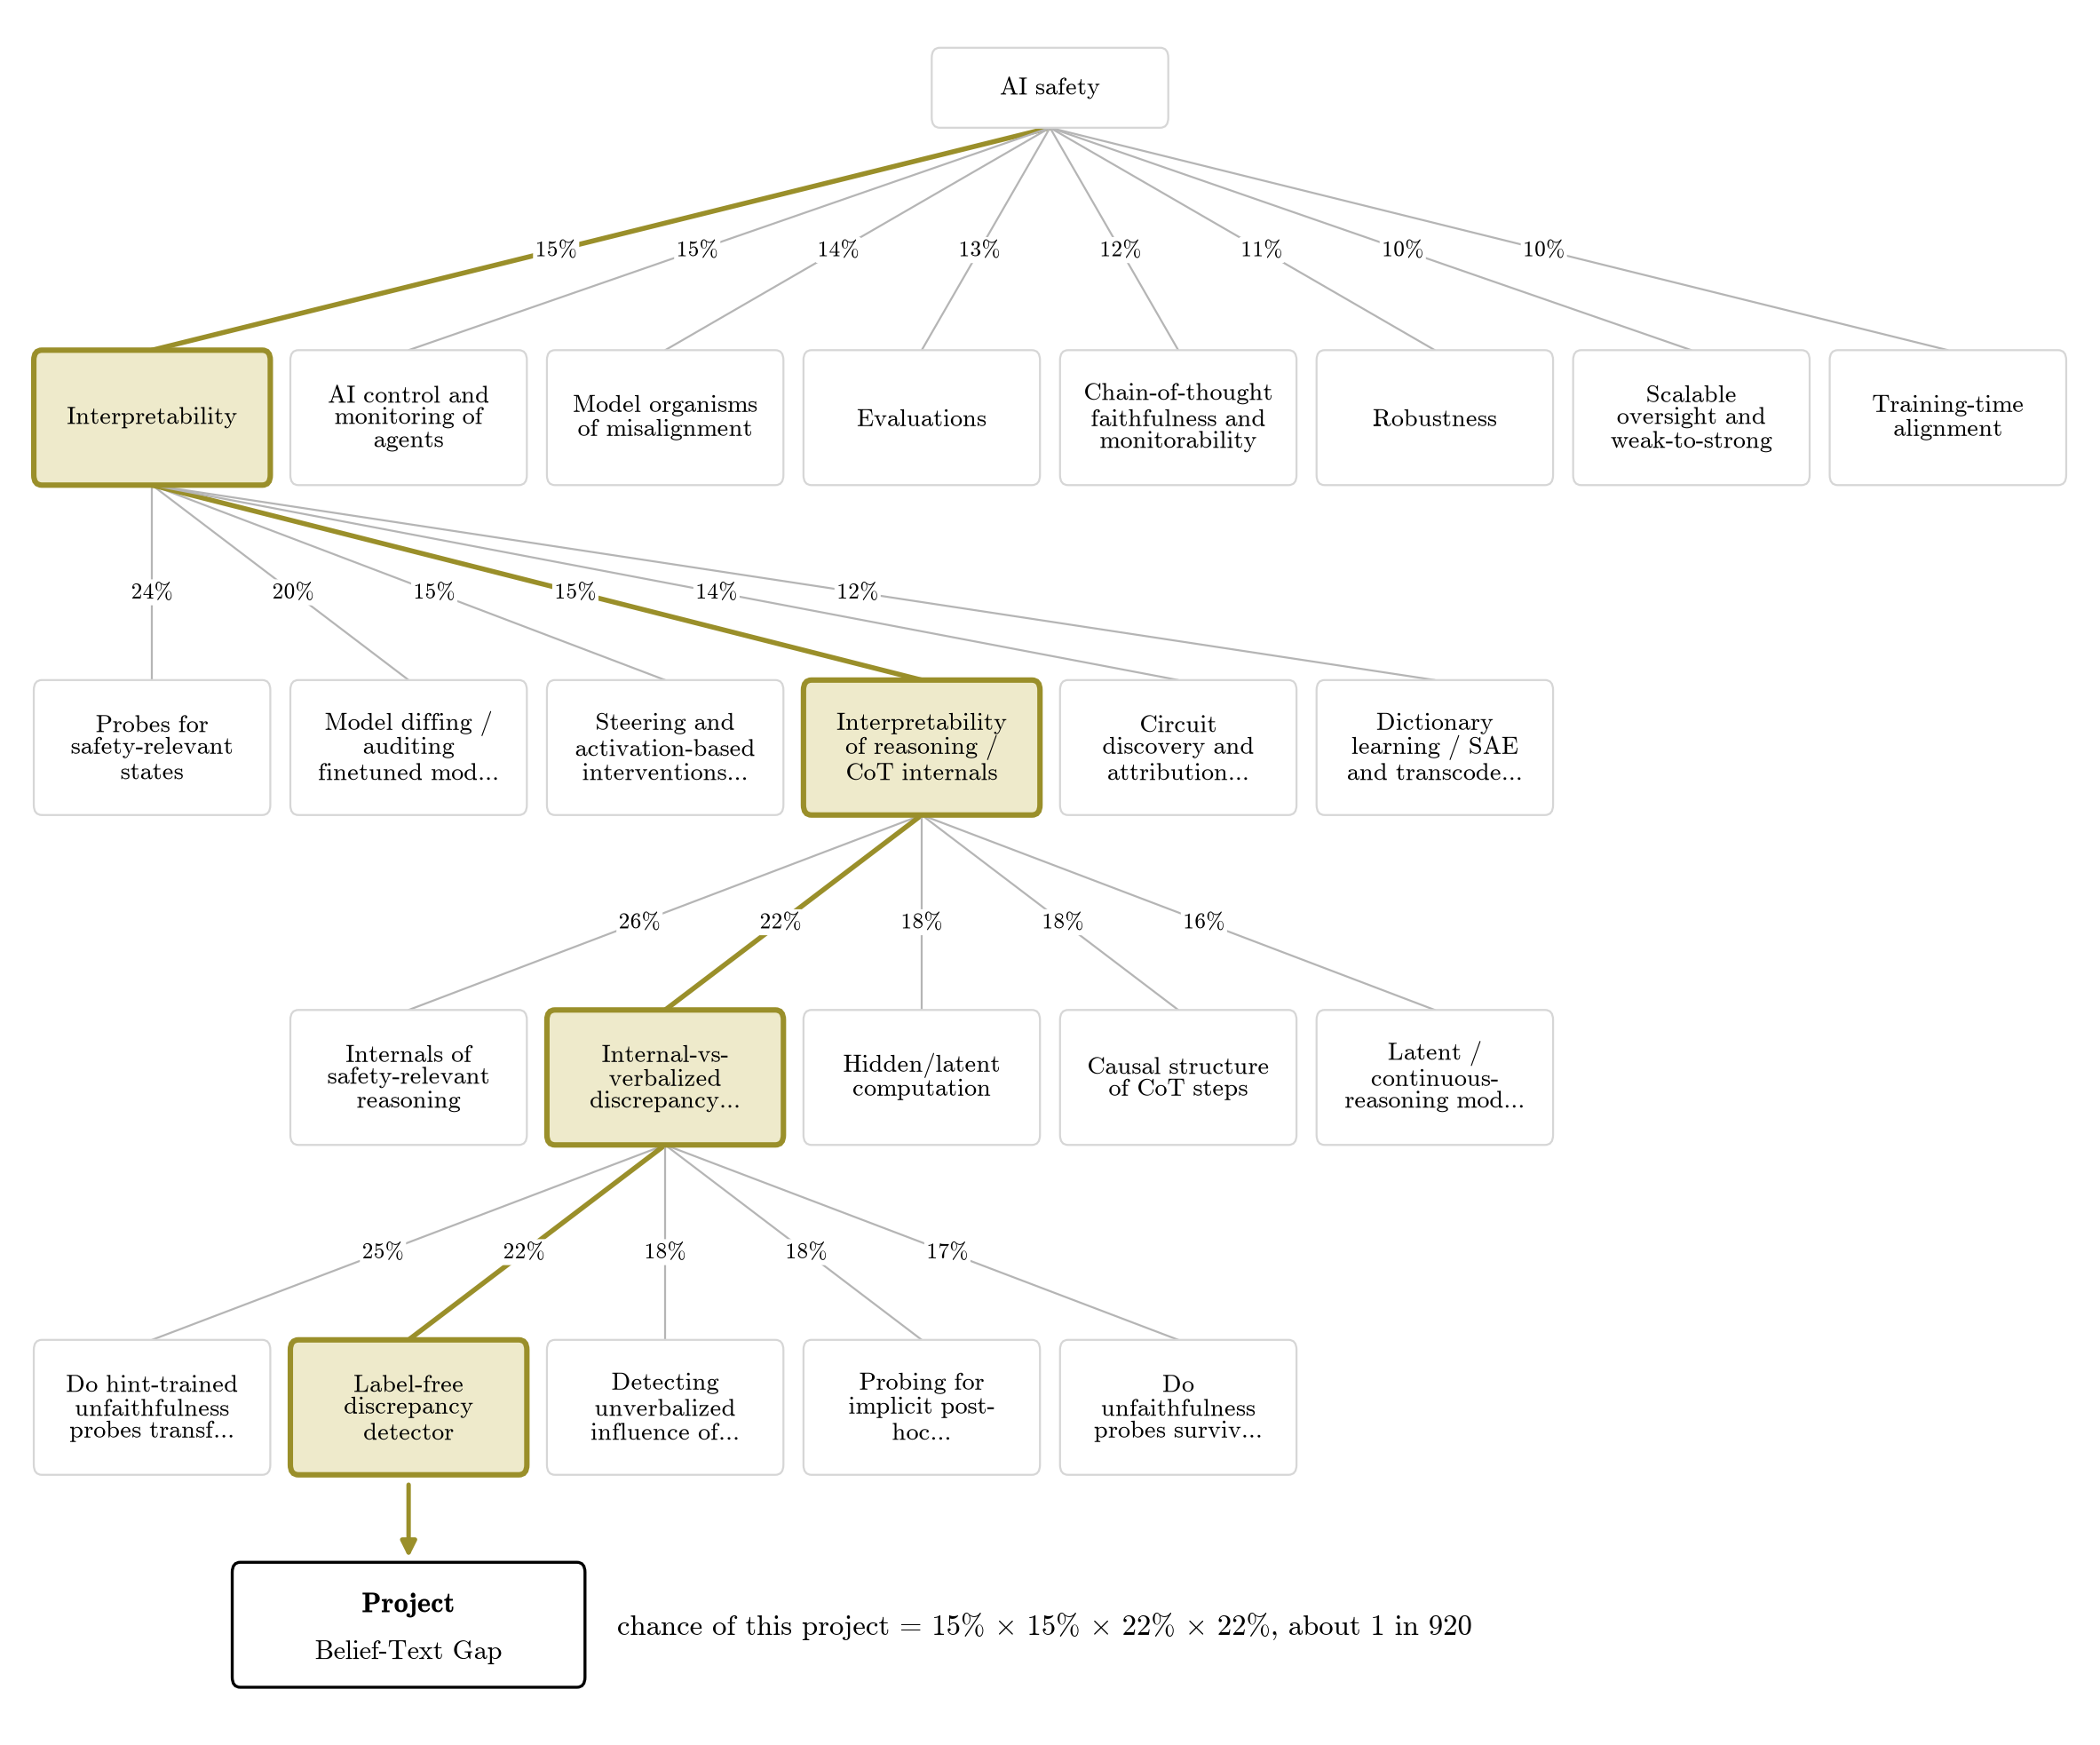
\includegraphics[keepaspectratio,alt={One frontier agent's walk down the tree (Opus 5.5 in Codex CLI), from its tool calls. Read top to bottom. From AI safety, a branch runs to each option the agent listed at its first draw, labelled with the weight the agent gave it, and each row is ordered from the highest weight on the left to the lowest. The branch the random draw returned is in the draw colour and splits into the next row of options, and the branches not drawn are grey. The chance of reaching the final project is the product of the percentages along its path. Labels are shortened.}]{figures/fig-tree-diagram.png}}
\caption{One frontier agent's walk down the tree (Opus 5.5 in Codex
CLI), from its tool calls. Read top to bottom. From AI safety, a branch
runs to each option the agent listed at its first draw, labelled with
the weight the agent gave it, and each row is ordered from the highest
weight on the left to the lowest. The branch the random draw returned is
in the draw colour and splits into the next row of options, and the
branches not drawn are grey. The chance of reaching the final project is
the product of the percentages along its path. Labels are
shortened.}\label{fig:10}
\end{figure}

\begin{figure}
\centering
\pandocbounded{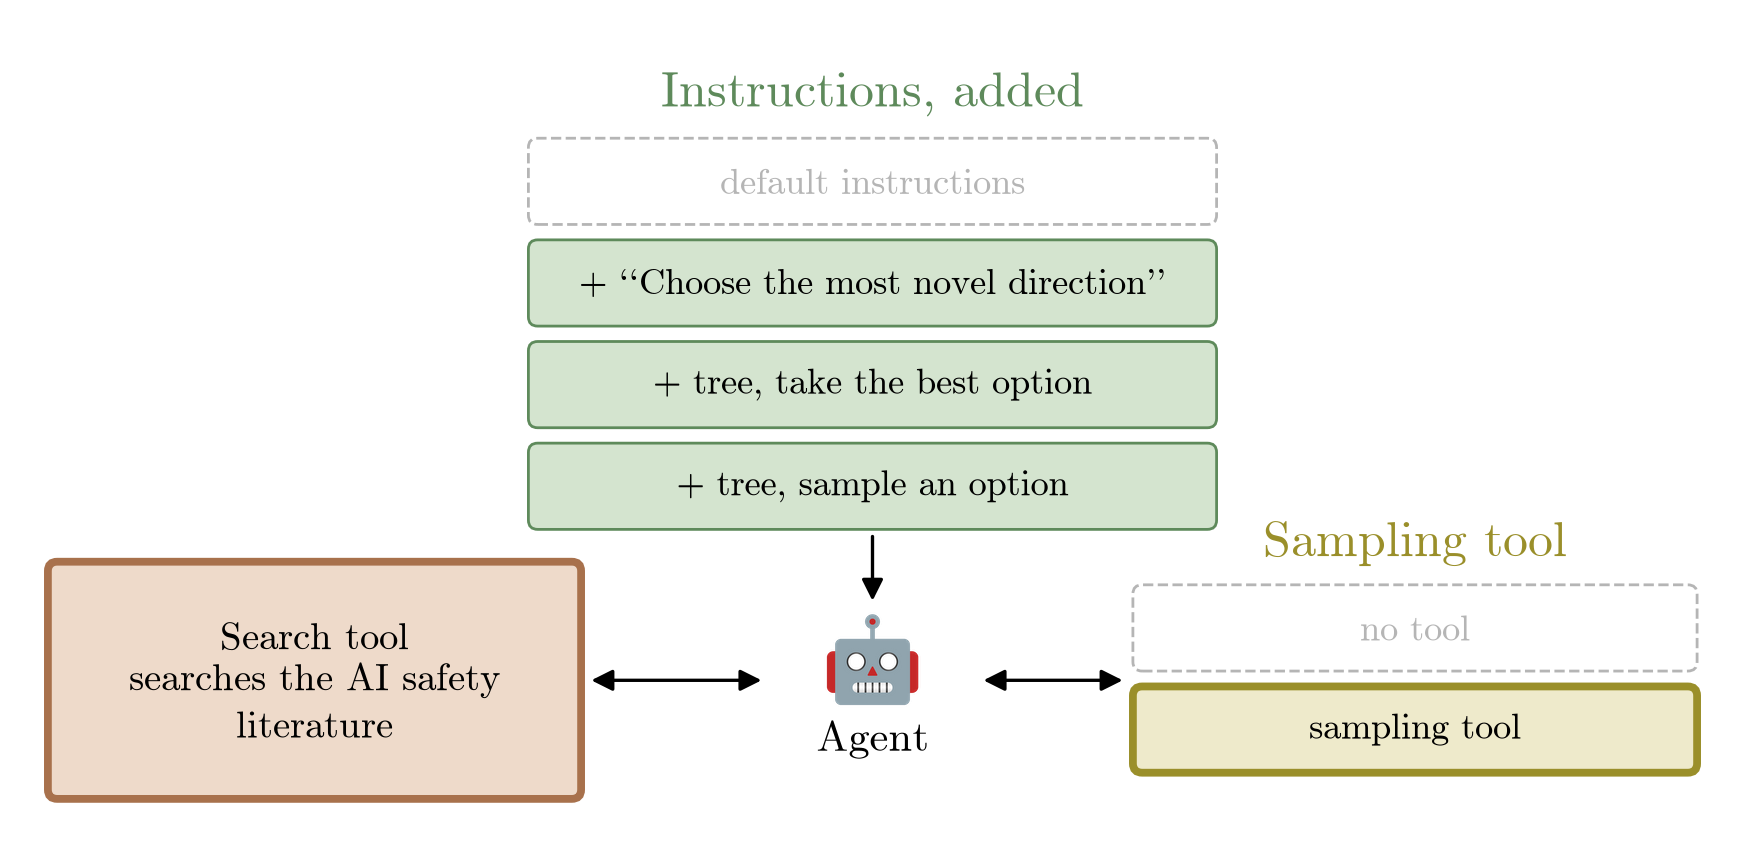
\includegraphics[keepaspectratio,alt={The setup for Section 7, drawn as Figure 1. Searching agents get their default instructions, a sentence asking for the most novel direction (``Choose the most novel direction you can find, one that few other researchers would pick.''), the tree protocol with the agent taking the option it judges best at each level, or the tree protocol with each option drawn at random by the random-draw tool. Only the last comes with the tool, which is bold because it contains randomness.}]{figures/fig-part3-setup.png}}
\caption{The setup for Section 7, drawn as Figure 1. Searching agents
get their default instructions, a sentence asking for the most novel
direction (``Choose the most novel direction you can find, one that few
other researchers would pick.''), the tree protocol with the agent
taking the option it judges best at each level, or the tree protocol
with each option drawn at random by the random-draw tool. Only the last
comes with the tool, which is bold because it contains
randomness.}\label{fig:11}
\end{figure}

\begin{figure}
\centering
\pandocbounded{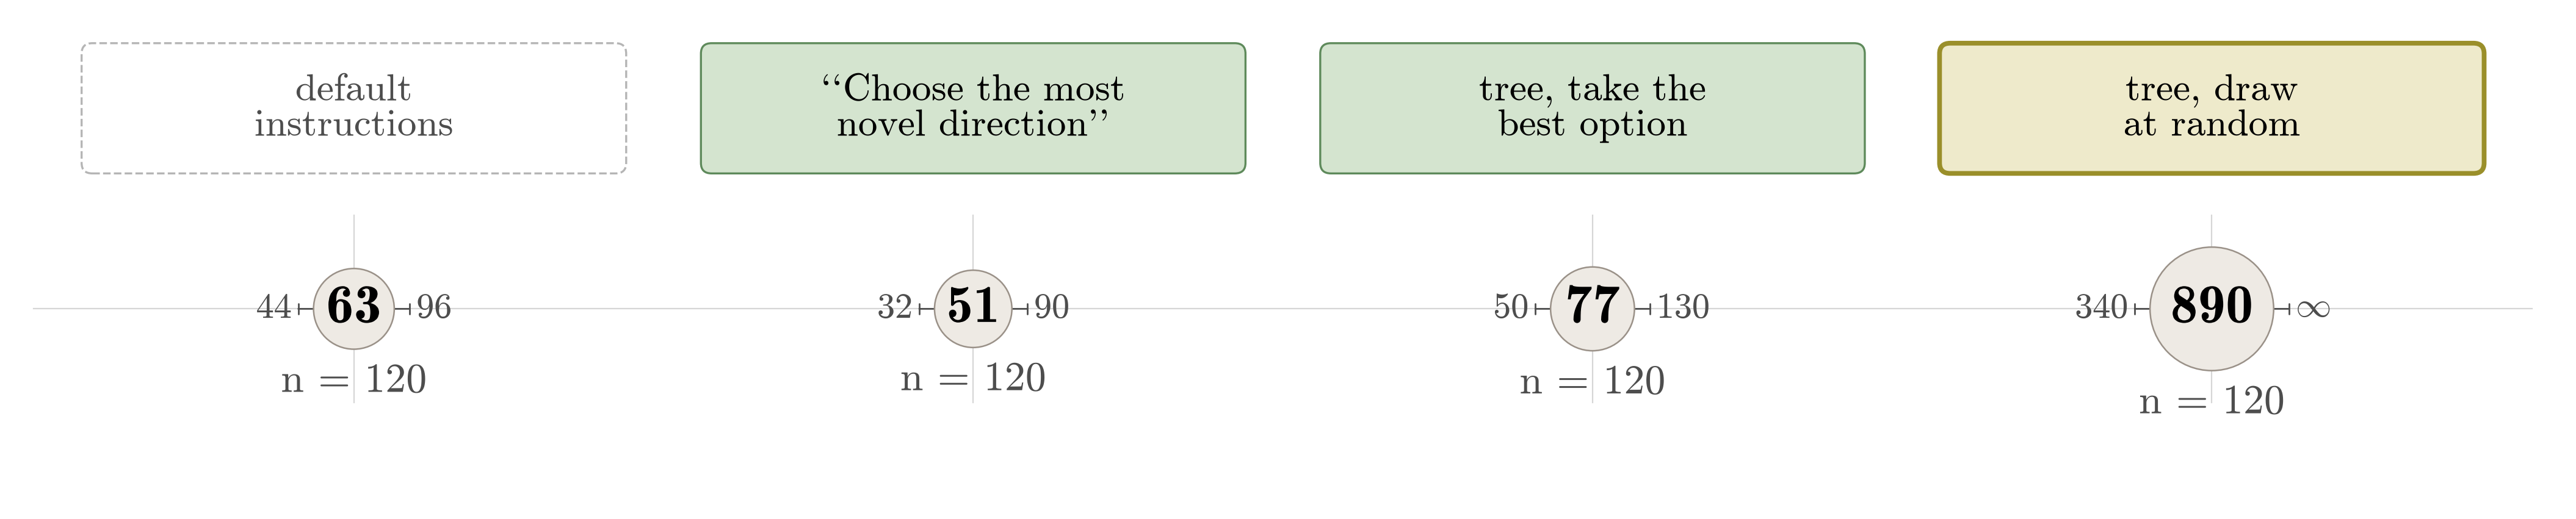
\includegraphics[keepaspectratio,alt={Drawn as Figure 4, on the same 120 combinations of model, launch prompt and harness, all searching: no added tool, the sentence quoted in Figure 11's caption, the tree with the agent taking the best option at each level, and the tree with each option drawn at random. The first row is Figure 4's searching agents choosing alone. The bold outline marks the one arm that draws at random.}]{figures/fig-15-protocol-pilot.png}}
\caption{Drawn as Figure 4, on the same 120 combinations of model,
launch prompt and harness, all searching: no added tool, the sentence
quoted in Figure 11's caption, the tree with the agent taking the best
option at each level, and the tree with each option drawn at random. The
first row is Figure 4's searching agents choosing alone. The bold
outline marks the one arm that draws at random.}\label{fig:12}
\end{figure}

Every agent called the random-draw tool without being reminded, drawing
2 to 6 times. With the protocol the field behaves like about 890
projects, against about 60 for the same combinations of model, launch
prompt and harness with no added tool, run the same day. The tree also
tripled the number of agendas the field spread over and cut AI control
from 59\% of picks with no added tool to 31\%. It spread agents in the
simple setup too, for an open model and for Claude Sonnet 5.5 answering
from memory (\hyperref[appendix-the-simple-setup]{appendix}).

Two more arms test which part of the protocol spreads agents (Figure
12). In one, agents got the same tree protocol but took the option they
judged best at each level instead of drawing, and the field was not
clearly more spread than with no tool. So the draws do most of the work.
One sentence asking for the most novel direction did not spread projects
either. Agents moved away from AI control but went to the same new
places. Twelve of 29 Claude Sonnet 5.5 agents, in all four harnesses,
proposed the same project, on whether the date tells a model it is
deployed or tested
(\hyperref[where-did-agents-go-when-asked-for-novelty]{appendix}).

The agents' own preferences played little role here. The frontier agents
weighted their options nearly evenly, giving the top option 1.3 to 1.5
times an equal share, as both models did from memory in the simple
setup. So each agent's draw was close to an even choice among its own
options. Our guess, which we have not tested, is that future models will
weight their options more sharply. Their draws would then concentrate on
the projects they rate highly, which would spread agents somewhat less.

The protocol can be adjusted for this. It calls the random-draw tool at
temperature 1, which draws each option in proportion to its weight. If
models that weight their options more sharply still produced too many
duplicates, a higher temperature would make the draw more even, and a
lower one would move it toward each agent's favourite. We expect a
higher temperature to lower the average quality of picks in exchange for
fewer duplicates, but we did not measure that.

The tree spreads agents because its picks are often not the model's
first choice, so agents give up some of their own preference. We do not
know how large that cost is.

\section{Limitations}\label{limits}

Today's models stand in for future ones, and we have not tested whether
the situation carries over.

We measure diversity only at the level of projects. Two agents count as
different whenever one's result would not largely answer the other's
question, even if both work on the same problem, so agents on many
different projects within one problem would score high and still be
narrow. A tree whose levels ran from agendas to questions to projects
could control how spread out agents are at each level. We think building
one is the most promising next step.

Every number depends on one language-model judge. Every label comes from
language models, checked against other models but not against people.
Most findings hold under every correction for the judge's misses that we
tried, and the few that do not are flagged in the appendix
(\hyperref[appendix-the-judge-and-how-far-to-trust-it]{the judge}).

Spreading a field is only worth it if the projects agents move to are
still good. We collected quality ratings from language models, but
today's models judge promise too weakly and inconsistently for these
ratings to say much, and no experts rated the picks, so we do not report
them. On pairs of AI safety proposals, the best model in a recent test
agreed with experienced researchers' judgements 60\% of the time,
against an estimated 77\% for the researchers themselves
\citep{baig2026taste}.

We tested seven models from four families and no Google models. No group
of people answered our exact brief. SPAR mentors answer the same
question implicitly, what a researcher should work on next in AI safety,
but they wrote for a program, and we do not know whether it screens
proposals for overlap, which would raise their number. Teams at four
broad-theme hackathons, whom no one screens, still behave like about 530
projects, far above agents choosing on their own. Search used our own
frozen copy of the literature, and temperature stayed at the provider
default. Our registries held at most 100 entries, and we do not know how
a registry behaves beyond 100 entries. It could become less effective,
for example if agents read less of a long list, or agents could start
copying each other more as more of the field is visible to them. We have
not tested this. The arms without search, with the novelty sentence, and
with agents taking the best option at each level ran a day after the
arms they are compared with.

\section{Related work}\label{related-work}

Language models give similar answers to open-ended questions, across
runs and across model families
\citep{jiang2025hivemind,wenger2025homogeneity,zhang2025noveltybench},
and their errors are correlated even across providers
\citep{kim2025correlated}. Preference training is one likely cause,
because it lowers the diversity of outputs \citep{kirk2024rlhf} and
favours typical answers \citep{zhang2025verbalized}. When many
decision-makers rely on one model, they can do worse together than if
each used its own, a problem known as algorithmic monoculture
\citep{kleinberg2021,bommasani2022}. People show the same pattern. Help
from AI makes each person's ideas better but everyone's ideas more alike
\citep{doshi2024,holzner2025metaanalysis}, and scientists who use AI
tools cover a narrower range of topics \citep{hao2026}, a risk that
\citet{messeri2024} describe as a monoculture of knowing. The evidence
is not all one way. Distances between models grew on most measures
across recent releases \citep{qiu2026homogeneity}, and for product
ideas, changing the prompt raised diversity \citep{meincke2024prompting}
and pooling vendors and prompts came close to people
\citep{terwiesch2026productideas}. Choosing a research project after
searching the literature, the task we study, is a different setting, and
there mixing models and prompts helped little.

Systems that carry out research from idea to paper now exist
\citep{lu2024,yamada2025aiscientistv2}, and research ideas from language
models lose more of their rated quality than people's once they are
carried out \citep{si2025execution}. Several studies compare the
research ideas of models and people. Ideas from AI research agents are
narrower than human papers across twelve fields \citep{tang2026narrow},
the kinds of idea models propose are more concentrated than people's
\citep{chenzhao2026gap}, and the methods models suggest for 1,000
research questions behave like 59 to 96 distinct methods against 1,232
in the published papers, by an effective number like ours
\citep{carlon2026methods}. Asked to pick one problem from a set, models
put more than half of their choices on the same problem, and mixing
models lowers that share only to about 40\% \citep{zhou2026alphaidea}.
Frontier models also agree with each other about which future research
directions to take, more so within one provider \citep{trehan2026taste}.
In alignment research itself, teams of automated researchers converged
on one training method for each failure they studied \citep{chenyh2026}.
Diversity matters for results too. Research agents whose ideas were made
less diverse won fewer medals on machine-learning tasks
\citep{audranreiss2025}. The closest study to ours is
IdeaTaste~\citep{zhong2026}, where assigning topics nearly doubled the
diversity of agents' research proposals and showing how crowded each
direction was in the published literature did not spread them. Other
work finds that frontier models give far more similar answers than human
scientists on a theory task \citep{li2026}, that grounding agents in the
same papers lowers the diversity of their ideas \citep{wang2026}, and
that 150 Claude Code agents analysing one dataset split their
conclusions by model and mostly switched to the approach of top-rated
analyses once shown them \citep{gao2026}.

Agents that see each other's choices tend to copy them, as people do in
markets for songs \citep{salganik2006} and in informational cascades
more generally \citep{bikhchandani1992}. Language-model agents follow
early leaders \citep{hashemi2026,cho2025}, conform more as the majority
grows \citep{weng2025conformity}, and converge on fewer ideas when they
discuss them \citep{chen2026}. Builders of multi-agent systems report
that parallel subagents duplicate each other's work unless a lead agent
divides it \citep{anthropic2025multiagent}. Several systems share state
to spread agents out. A board of claimed directions spread four Claude
Code agents doing research \citep{ren2026coral}, a persistent memory
widened the changes an autonomous research loop tried
\citep{he2026beneath}, a central repository of AI-generated hypotheses
has been proposed for AI scientists \citep{bisht2026agentic}, and
DivAlign~\citep{xu2026} spreads AI-suggested directions across 95
researchers by cutting overlap. Our registry is the simplest of these, a
list each agent reads before choosing, and we compare it with people
choosing in the same field.

The question of how a field should divide its effort is old.
Philosophers of science argue that a community does better when some
researchers work on options that look less promising
\citep{kitcher1990,weisberg2009,thoma2015}, and that a community
converging too fast can lock onto the wrong option \citep{zollman2010}.
Economists find that competing firms choose research projects that are
too alike \citep{dasgupta1987}. Among people, credit for being first
pushes researchers away from crowded problems
\citep{strevens2003,kleinberg2011}, though scientists' choices are still
more conservative than would be best for discovery
\citep{foster2015,rzhetsky2015}. Agents choosing a project have no such
incentive, which is one reason to expect them to crowd more than people
do.

Drawing at random among options that are good enough is already used to
fund research \citep{fang2016,avin2019,heyard2022}, and randomness has
been proposed as a guard against one arbitrary decision rule applied
everywhere \citep{creel2022}. Drawing each option with the probability
one assigns to it is probability matching, the rule behind Thompson
sampling \citep{thompson1933,russo2018thompson}. For language models,
asking for a list of answers with probabilities raises the diversity of
outputs \citep{zhang2025verbalized}, listing options and then picking
one makes copies of a model agree with each other less
\citep{ballestero2026}, and planning a spread of directions in one call
works well \citep{ibrahim2026anchorless}. Models cannot do the drawing
themselves, because they fail tests of random sampling
\citep{zhao2026dice} and repeat human biases when asked to flip coins
\citep{vankoevering2024coinflips}. The tree protocol therefore hands the
draw to a tool and repeats it level by level, so each agent keeps its
own weights and no shared service is needed. In one simulation, adding
randomness helped a community only when its problems could be split into
parts \citep{fazelpour2026}.

Within one field and with one measure, we compare the setup choices that
differ between labs, such as model, launch prompt and harness, with each
other and with people choosing projects in the same field. As far as we
know, two results are new. Searching the literature spreads frontier
agents' projects but crowds them onto fewer problems, and a sentence
asking for novelty, which spread an open model answering from memory,
moved frontier agents together onto new projects instead of spreading
them, a pattern also seen for one-word answers \citep{parikh2026}. In
another study, an instruction to differ from the rest of the population
did help \citep{ibrahim2026anchorless}. The tree protocol needs no
shared service and leaves the choice with the agent. Assigning topics,
the other intervention shown to work, takes that choice away.

\bibliographystyle{plainnat}
\bibliography{refs}
\clearpage
\appendix
\renewcommand{\thefigure}{A\arabic{figure}}\setcounter{figure}{0}

\section{What we ran}\label{appendix-what-we-ran}

All runs took place between 8 and 18 November 2026. The seven agent
models are GLM-5.3-flash, GLM-5.3, DeepSeek V4.1 Flash (also the judge),
Claude Sonnet 5.5, Claude Opus 5.5, GPT-6 Astra and GPT-6.1 Sol. Every
agent got one session and named one project. Claude Code was version
2.1.319, Codex CLI 0.167.0 and opencode 1.19.5, and the minimal loop is
a short tool-calling loop of our own.

{\def\LTcaptype{none} % do not increment counter
\begin{longtable}[]{@{}
  >{\raggedright\arraybackslash}p{(\linewidth - 4\tabcolsep) * \real{0.2308}}
  >{\raggedright\arraybackslash}p{(\linewidth - 4\tabcolsep) * \real{0.5385}}
  >{\raggedright\arraybackslash}p{(\linewidth - 4\tabcolsep) * \real{0.2308}}@{}}
\toprule\noalign{}
\begin{minipage}[b]{\linewidth}\raggedright
Figures
\end{minipage} & \begin{minipage}[b]{\linewidth}\raggedright
Setup
\end{minipage} & \begin{minipage}[b]{\linewidth}\raggedright
Agents
\end{minipage} \\
\midrule\noalign{}
\endhead
\bottomrule\noalign{}
\endlastfoot
A11, A13, A15 & Step one, the simple setup's first experiment:
GLM-5.3-flash, minimal loop, our brief; from memory, two assigned
reading lists, and search with three levels of randomness & 120 per
cell, 240 in two search cells \\
A11 & One change at a time from step one's memory cell: seven models;
our loop, Codex CLI, opencode; four launch prompts; and every change at
once & 40 per group, 120 for every change at once \\
A13 & Step one's reading conditions for six more models & 40 per cell \\
A13 & The frontier setup: four frontier models, each in the harnesses it
runs in, eleven launch prompts (our brief, counting its two slightly
different lengths as one, and ten others), search & 80, plus 80 with the
interpretability brief (appendix) \\
A15 & Registry, first stage: GLM-5.3-flash from memory; registry of
earlier projects, agenda counts, placebo & \(4 \times 100\) per
registry, 200 placebo \\
A15 & The first stage's registry of earlier projects re-judged on every
pair & \(4 \times 100\) \\
A8, text & Registry, first frontier test: registry of earlier projects
against placebo & \(6 \times 20\) per arm \\
text & Registry, first frontier test: agenda counts (run 16 November) &
\(6 \times 20\) \\
2, 4, 6, 8, 9, 12, A2-A5, A7 & The frontier setup with no added tool:
the same 120 combinations of model, launch prompt and harness as the
frontier registry test, with no added tool (run 16 November) & 120 \\
A15 & Tree protocol in the simple setup: GLM-5.3-flash from memory, with
and without the protocol & 120 per arm, plus 179 more agents with it \\
A15 & Repeat of the simple setup with Claude Sonnet 5.5: about 16
projects without the protocol (12 to 21), about 550 with it (250 to
2,400), 34 times as many (15 to 170) & 120 per arm \\
6 & The frontier setup's same 120 combinations of model, launch prompt
and harness with no search tools (run 17 November) & 120 \\
12 & The frontier setup's same 120 combinations of model, launch prompt
and harness with the novelty sentence, and with the tree protocol but
the agent taking the best option at each level instead of drawing (run
17 November) & 120 per arm \\
4, 8, 9 & Registry in the frontier setup, populations of 100: registry
of earlier projects, agenda counts and placebo (run 17 November) &
\(3 \times 100\) per arm \\
A5 text & Assigned first document: the frontier setup's same 120
combinations of model, launch prompt and harness plus 40 more, each
handed one of four papers as the top result of its first search (run 18
November) & \(4 \times 40\) \\
4, 10, 12 & Tree protocol in the frontier setup (run 16 November),
against the placebo arm of the first frontier registry test (run 14
November) & 120 per arm \\
4, A1 & People: SPAR mentor proposals, AI safety papers and LessWrong
posts from 2025 and 2026, six hackathons & 16 random groups of 40 per
source or event \\
\end{longtable}
}

\section{The judge and how far to trust
it}\label{appendix-the-judge-and-how-far-to-trust-it}

The judge is DeepSeek V4.1 Flash with the prompt in the
\href{https://github.com/AverroesLabs/ai-research-agent-diversity/blob/main/prompts/README.md}{prompts
appendix}. Each pair is judged in both orders, and it counts as a
duplicate when both say same project, or one says same project and the
other same direction. To save cost, pairs whose texts are far apart by a
small embedding model are counted as different without asking the judge.
The main text judged every pair of agents, which catches more
duplicates. In the simple setup, Figures A11 and A13 and one row of
Figure A15 use the screened judging. Shorter texts look more alike to
the judge, so drawn projects, which are written more briefly, are if
anything counted as duplicates more often.

Against blind labels from a Claude model, the judge agrees on duplicates
with a Cohen's \(\kappa\) of 0.60 to 0.76 and misses about 30\% of
agents' duplicates. How many it misses varies a little by model.
Corrected for its misses, every model's number changes by a factor of
0.7 to 1.1. For the GPT models, which have no hand labels, it can fall
to 0.6 under the most pessimistic assumption. No comparison in the paper
reverses, though three comparisons in our full results become ties under
some corrections. The pilot brief is an earlier version of our brief
with one more sentence, described in the simple-setup appendix. Every
model stays at 3 to 8 projects from memory on the pilot brief. Its
screening step drops some of agents' duplicates but none of people's, so
it can only overstate how spread agents are. In the simple setup the
judge misses more duplicates than it invents, so there it makes groups
look more spread out than they are. In the frontier setup a Claude and a
GPT labeller checked it blind and agreed with each other at
\(\kappa = 0.79\) on 90 pairs. Of 31 pairs the judge called duplicates,
30 were the same project or borderline for both, but about a quarter
were borderline. Counting only clear duplicates would raise the frontier
numbers about 1.3 times, counting borderline pairs too would lower them
by about a third, and no comparison the paper treats as settled would
reverse. Its misses inflate people's numbers most, because people have
almost no duplicates: allowing for them, people's lower bounds fall to
between about 150 and 1,000, well above every agent group answering from
memory. The most spread agent groups, searching or asked for novelty,
come close to those corrected bounds, but their own numbers are
uncorrected and would also fall if corrected.

Groups drawn in Figure 2(a) and (b) are approximate, because the judge
decides pair by pair and two projects can each match a third without
matching each other. The effective number comes from the pairs directly.

\section{People rarely repeat a
project}\label{appendix-people-rarely-repeat-a-project}

To know whether an agent number is high or low, we measured groups of 40
drawn from people's work: AI safety papers and LessWrong posts from 2025
and 2026, mentor proposals from the \href{https://sparai.org}{SPAR}
research program, and team projects from six
\href{https://apartresearch.com}{Apart} hackathons.

\begin{figure}
\centering
\pandocbounded{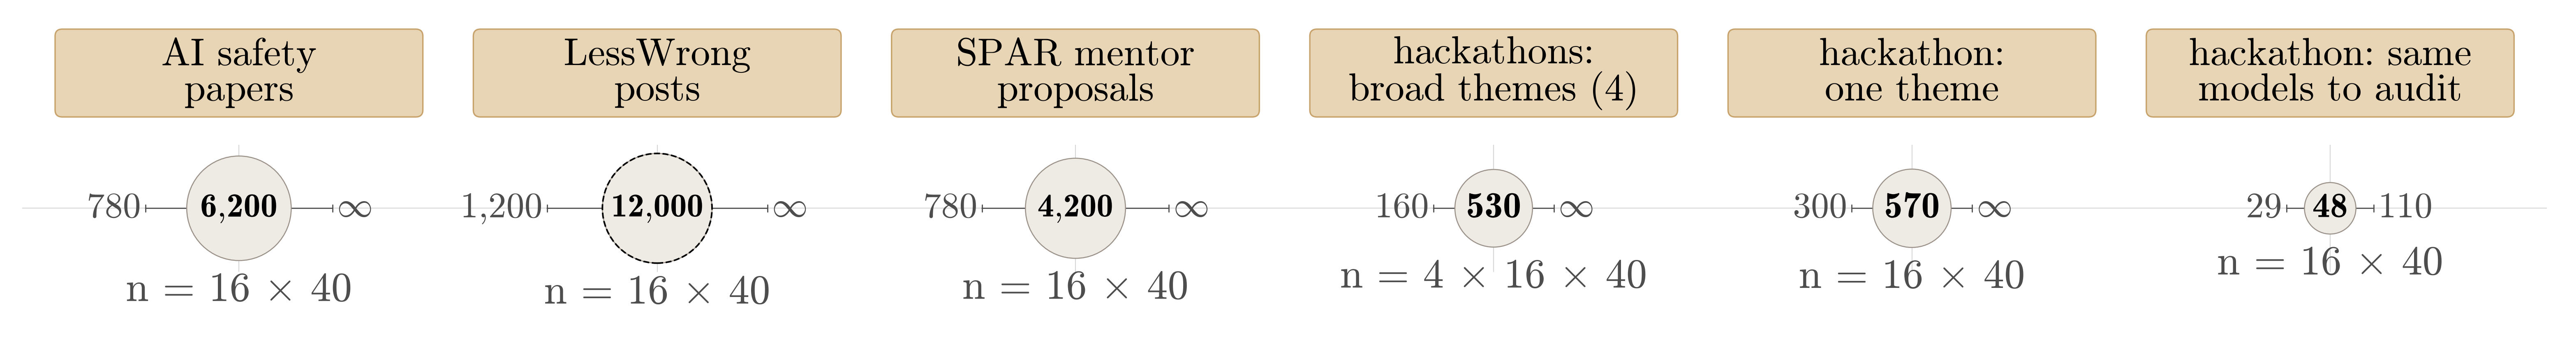
\includegraphics[keepaspectratio,alt={One row per source of people's work, drawn as Figure 4. Each circle is the effective number of projects, pooled over 16 random groups of 40, and its interval is the middle 95\% of the groups' own values. An arrow means some groups had no repeats at all, so the interval has no upper end. The broad-theme row pools four hackathons whose teams chose freely within a wide theme (Global South AI Safety 2026, def/acc 2025, AI Manipulation 2026 and Digital Minds 2026), each event weighted equally and its interval taken over all 64 groups. The other two hackathons fixed more: one gave every team one theme, the other also gave every team the same models to audit. To save cost, people's pairs were screened before judging, skipping pairs whose texts are far apart; on people this missed no duplicate that judging every pair found.}]{figures/fig-02-people.png}}
\caption{One row per source of people's work, drawn as Figure 4. Each
circle is the effective number of projects, pooled over 16 random groups
of 40, and its interval is the middle 95\% of the groups' own values. An
arrow means some groups had no repeats at all, so the interval has no
upper end. The broad-theme row pools four hackathons whose teams chose
freely within a wide theme (Global South AI Safety 2026, def/acc 2025,
AI Manipulation 2026 and Digital Minds 2026), each event weighted
equally and its interval taken over all 64 groups. The other two
hackathons fixed more: one gave every team one theme, the other also
gave every team the same models to audit. To save cost, people's pairs
were screened before judging, skipping pairs whose texts are far apart;
on people this missed no duplicate that judging every pair
found.}\label{fig:A1}
\end{figure}

People almost never repeat each other. Mentor proposals and published
work behave like thousands of projects, and hackathon teams, whom no one
screens for overlap, like several hundred. Teams across four broad-theme
events behave like about 530, from about 330 to 2,100 per event, and
teams given one theme like about 570. A measure that uses no judge, how
far apart the texts sit in an embedding model, also puts the broad-theme
and one-theme hackathons above every agent group, while the hackathon
with shared models to audit sits at the top of the agents' range. Only
when organizers handed every team the same models to audit does the
number fall, to about 50, and there the convergence was built into the
brief.

\section{Inside the frontier
setup}\label{appendix-inside-the-frontier-setup}

These sections look inside the frontier setup's runs, in the order of
Sections 5--7.

\subsection{Each model on its own}\label{each-model-on-its-own}

\begin{figure}
\centering
\pandocbounded{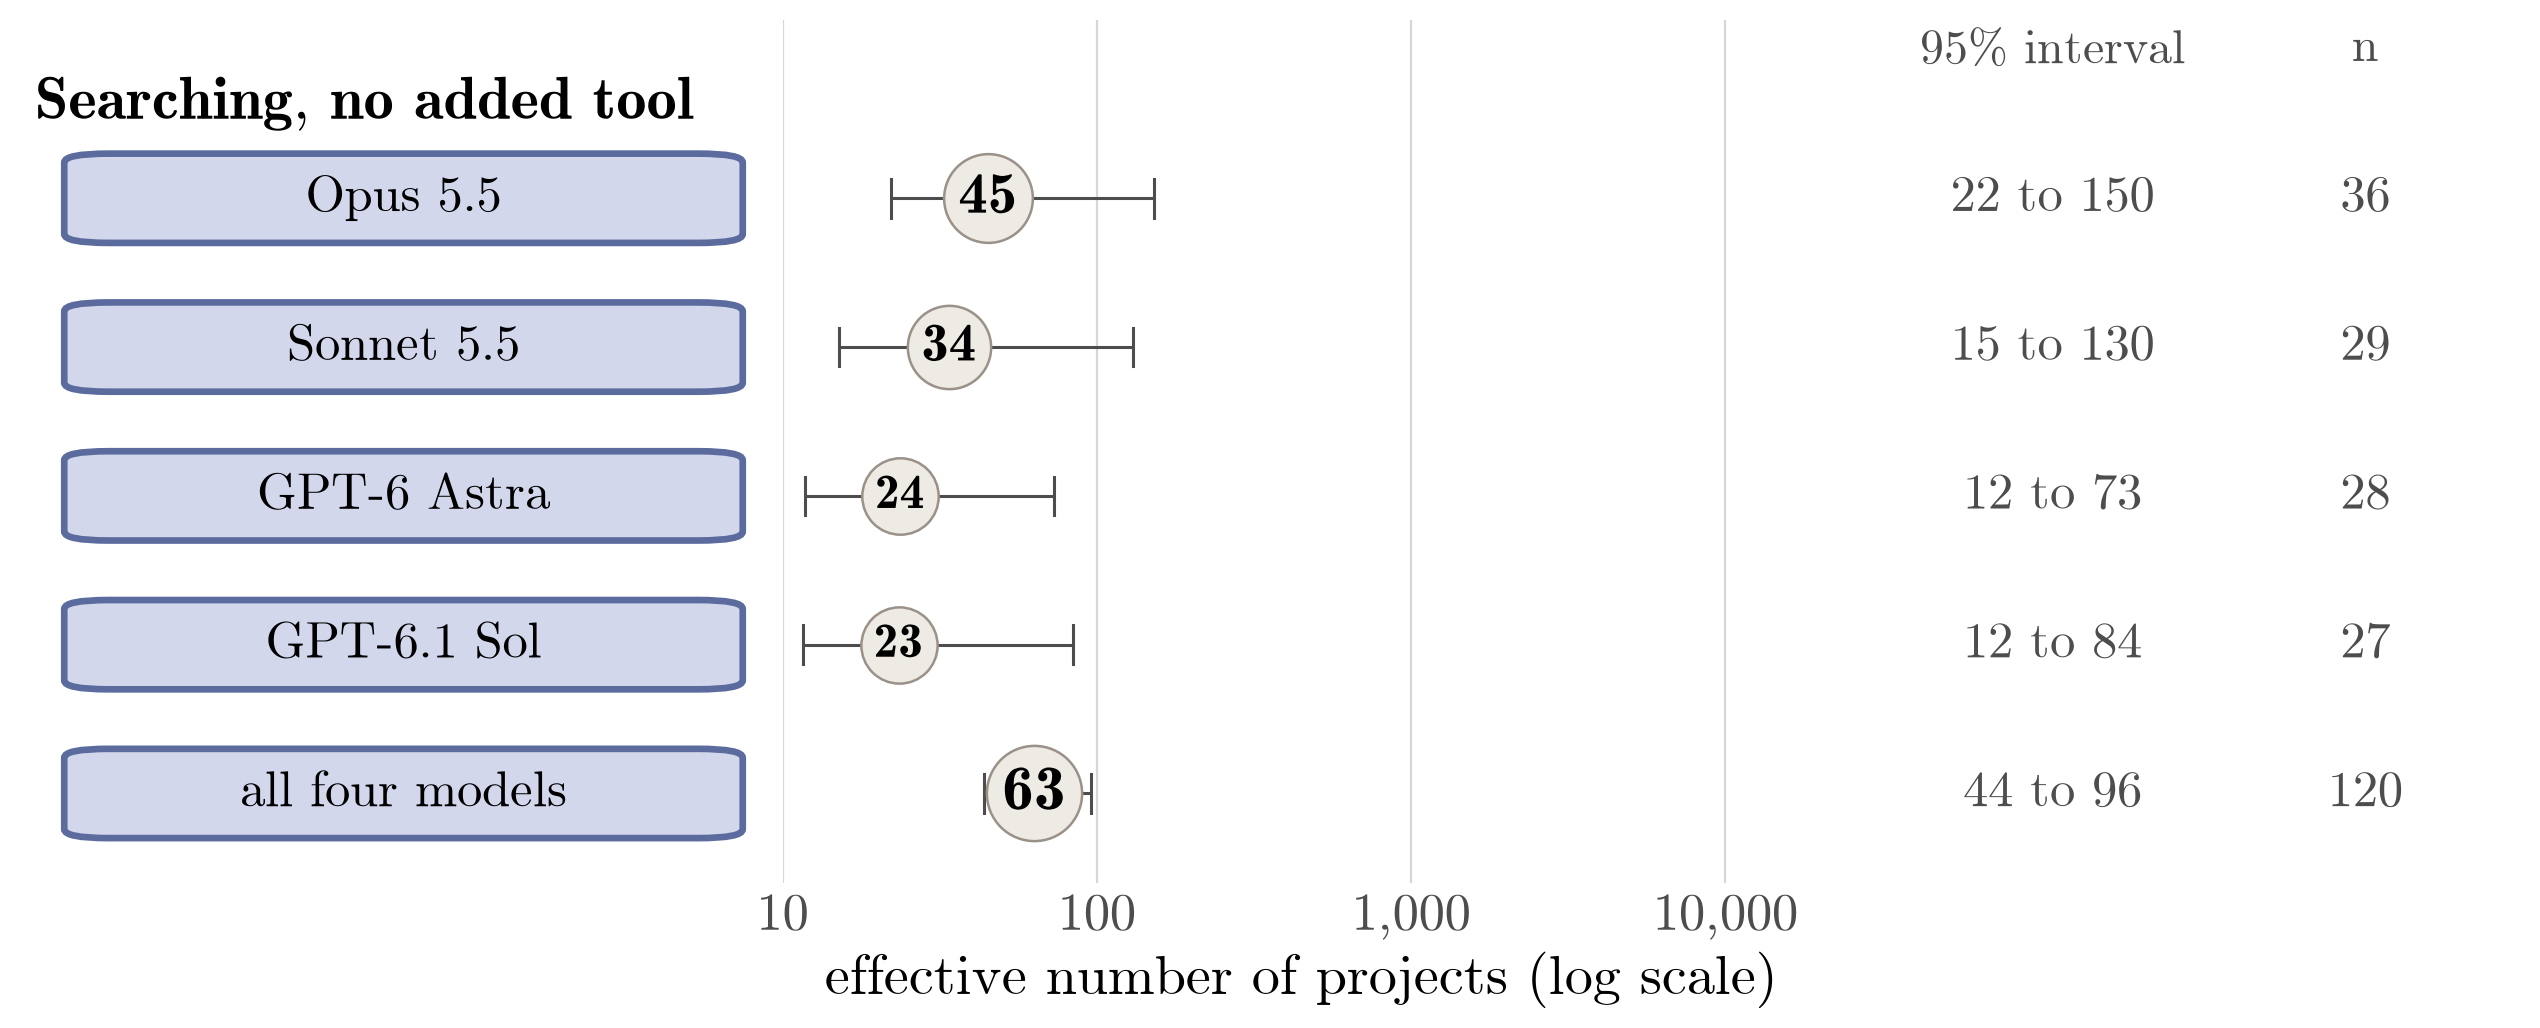
\includegraphics[keepaspectratio,alt={Drawn as Figure 4, one row per model. Each of the first four rows is one model's agents within the frontier setup's no-tool run, still with the launch prompts and harnesses that model got, and searching, counting only pairs between agents of that model. The last row is all 120 agents, Figure 4's searching agents choosing alone. Every pair of agents is judged, and intervals are 95\%, from resampling agents.}]{figures/fig-field-models.png}}
\caption{Drawn as Figure 4, one row per model. Each of the first four
rows is one model's agents within the frontier setup's no-tool run,
still with the launch prompts and harnesses that model got, and
searching, counting only pairs between agents of that model. The last
row is all 120 agents, Figure 4's searching agents choosing alone. Every
pair of agents is judged, and intervals are 95\%, from resampling
agents.}\label{fig:A2}
\end{figure}

\subsection{Do different models choose the same
projects?}\label{do-different-models-choose-the-same-projects}

\begin{figure}
\centering
\pandocbounded{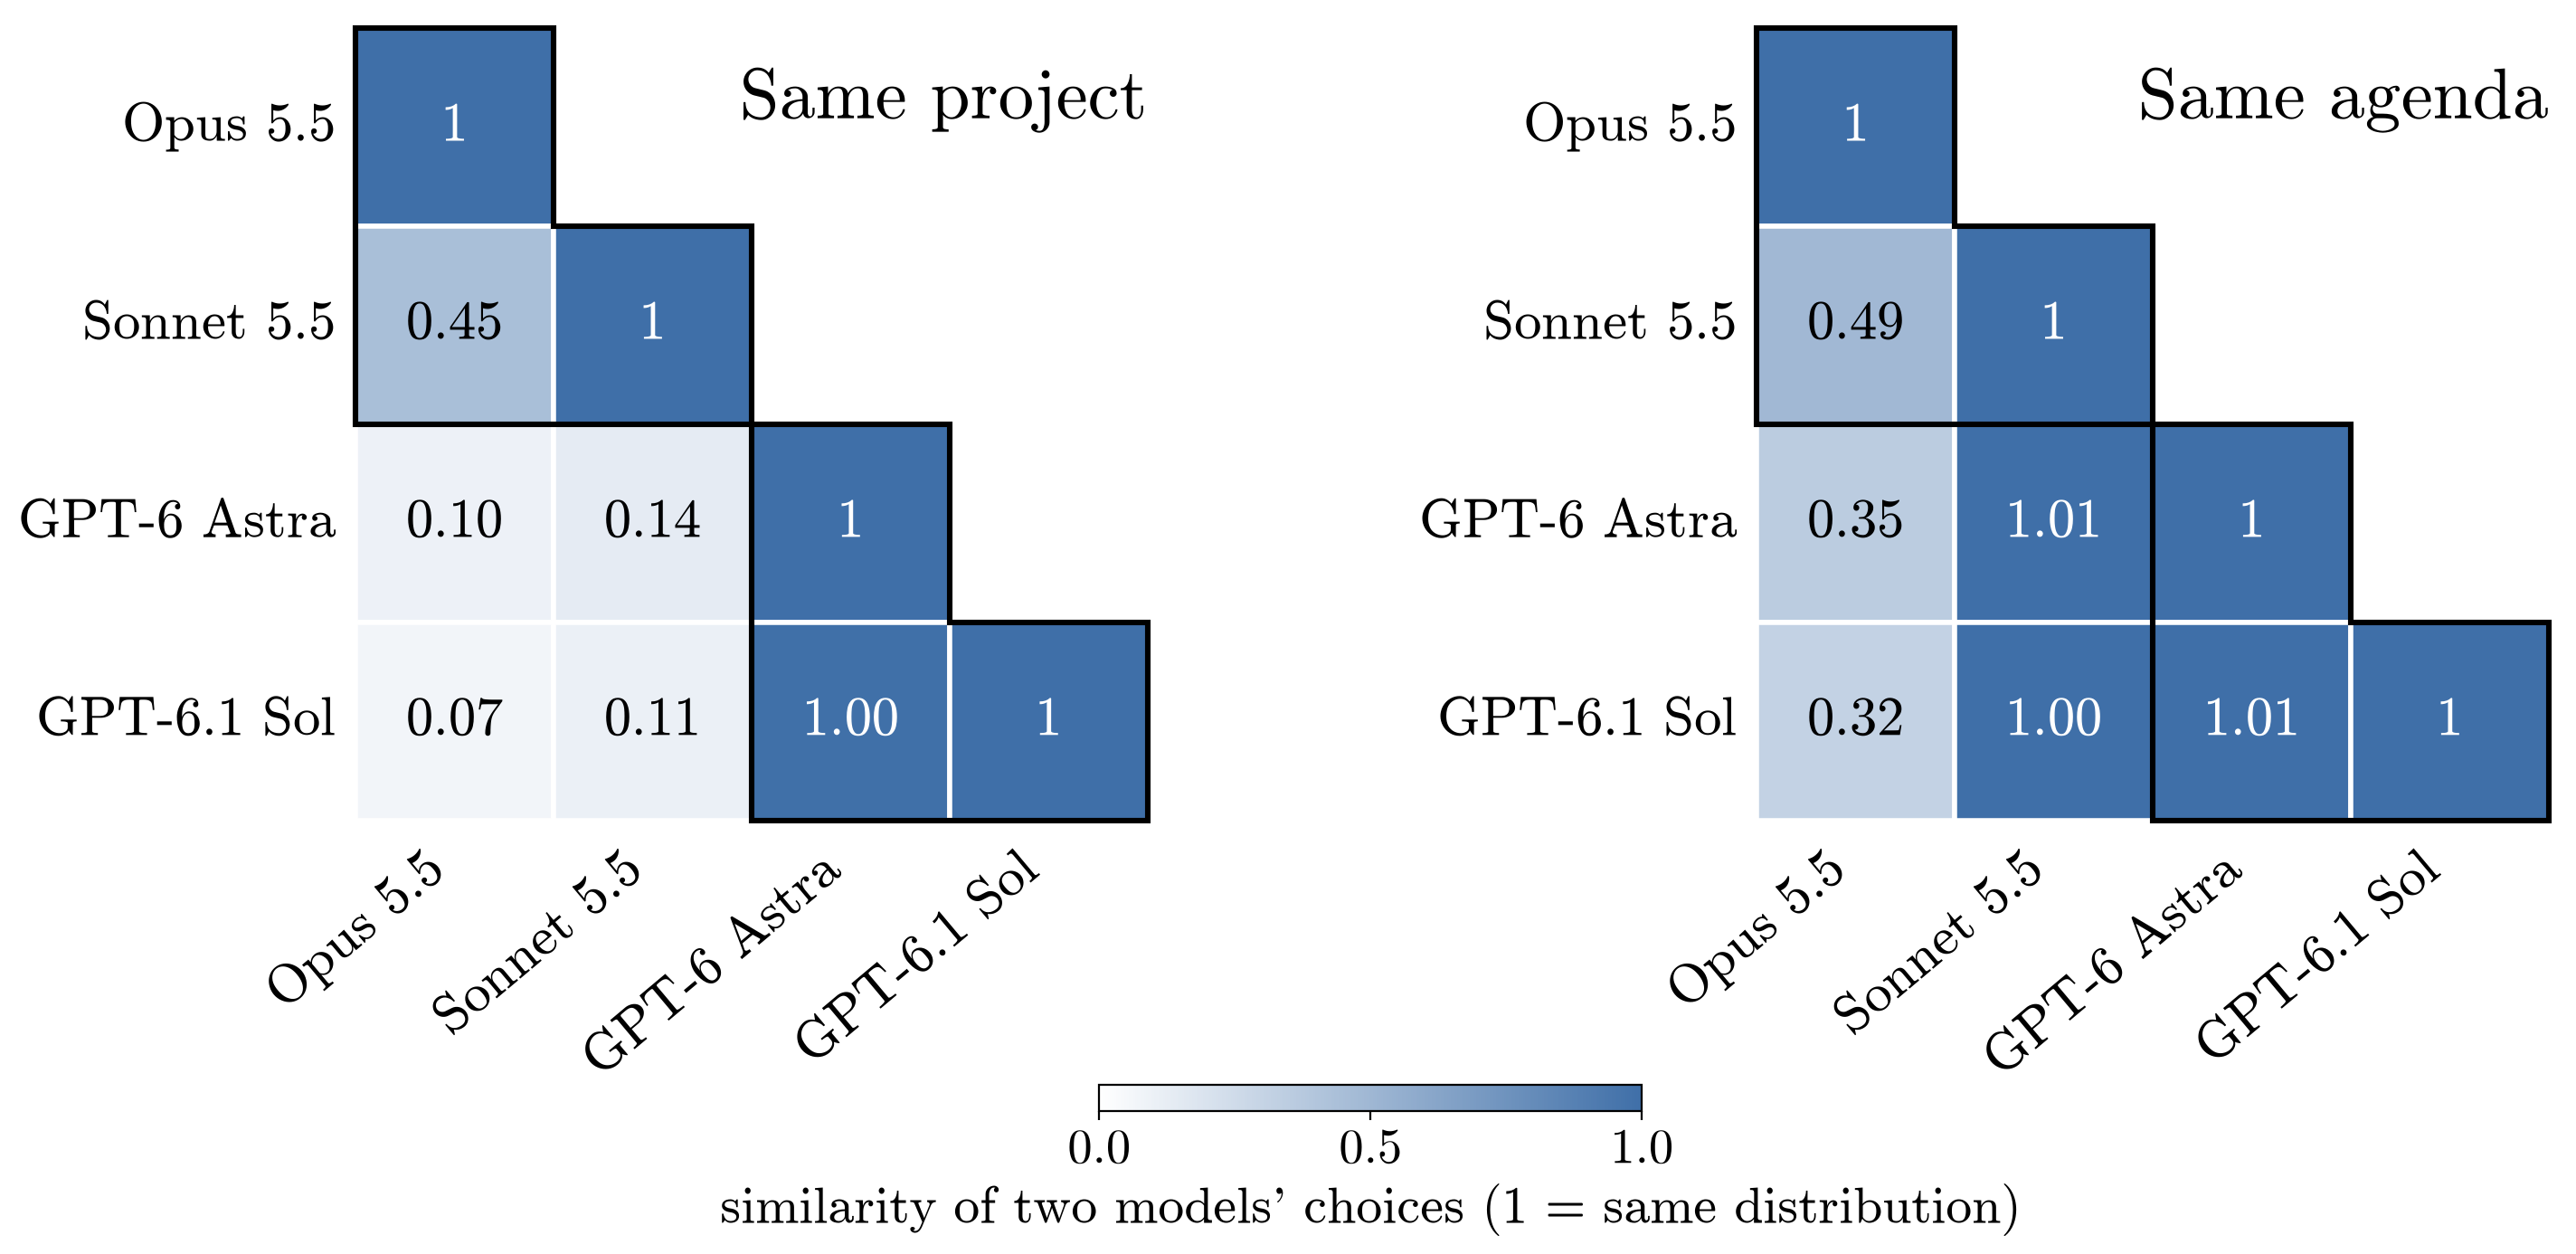
\includegraphics[keepaspectratio,alt={How alike two models' choices are in the frontier setup's no-tool run, about 30 agents per model, each with its own launch prompts and harnesses, and searching. Each cell is the chance that an agent of one model and an agent of the other match, divided by the geometric mean of the chance that two agents of each model match each other. That is the similarity of the two models' choice distributions: 1 means they pick from the same distribution, 0 that they never pick the same thing. Left, matching on projects as the judge decides; right, matching on agendas, with the labels of Figure A6. Outlines mark model families. Values can slightly exceed 1 by chance.}]{figures/fig-A-field-triangles.png}}
\caption{How alike two models' choices are in the frontier setup's
no-tool run, about 30 agents per model, each with its own launch prompts
and harnesses, and searching. Each cell is the chance that an agent of
one model and an agent of the other match, divided by the geometric mean
of the chance that two agents of each model match each other. That is
the similarity of the two models' choice distributions: 1 means they
pick from the same distribution, 0 that they never pick the same thing.
Left, matching on projects as the judge decides; right, matching on
agendas, with the labels of Figure A6. Outlines mark model families.
Values can slightly exceed 1 by chance.}\label{fig:A3}
\end{figure}

Models from the same company choose similar projects. The two GPT models
pick their projects from the same distribution, and the two Claude
models overlap about halfway. Between families, project overlap is
small, a tenth or so. Agendas overlap far more: Sonnet and the GPT
models work on the same problems in the same proportions, while Opus
stands apart. The same families appear with seven models answering from
memory in the simple setup, where the two GLM models also pick from
closely related distributions and the GPT models almost never share a
project with any other family. A few projects there are chosen by five
different models, such as ``Does Evading One Monitor Mean Evading Both?
Cross-Monitor Transfer of Obfuscation in RL-Trained Reward Hackers''.

\subsection{Do launch prompts or harnesses make agents
alike?}\label{do-launch-prompts-or-harnesses-make-agents-alike}

\begin{figure}
\centering
\pandocbounded{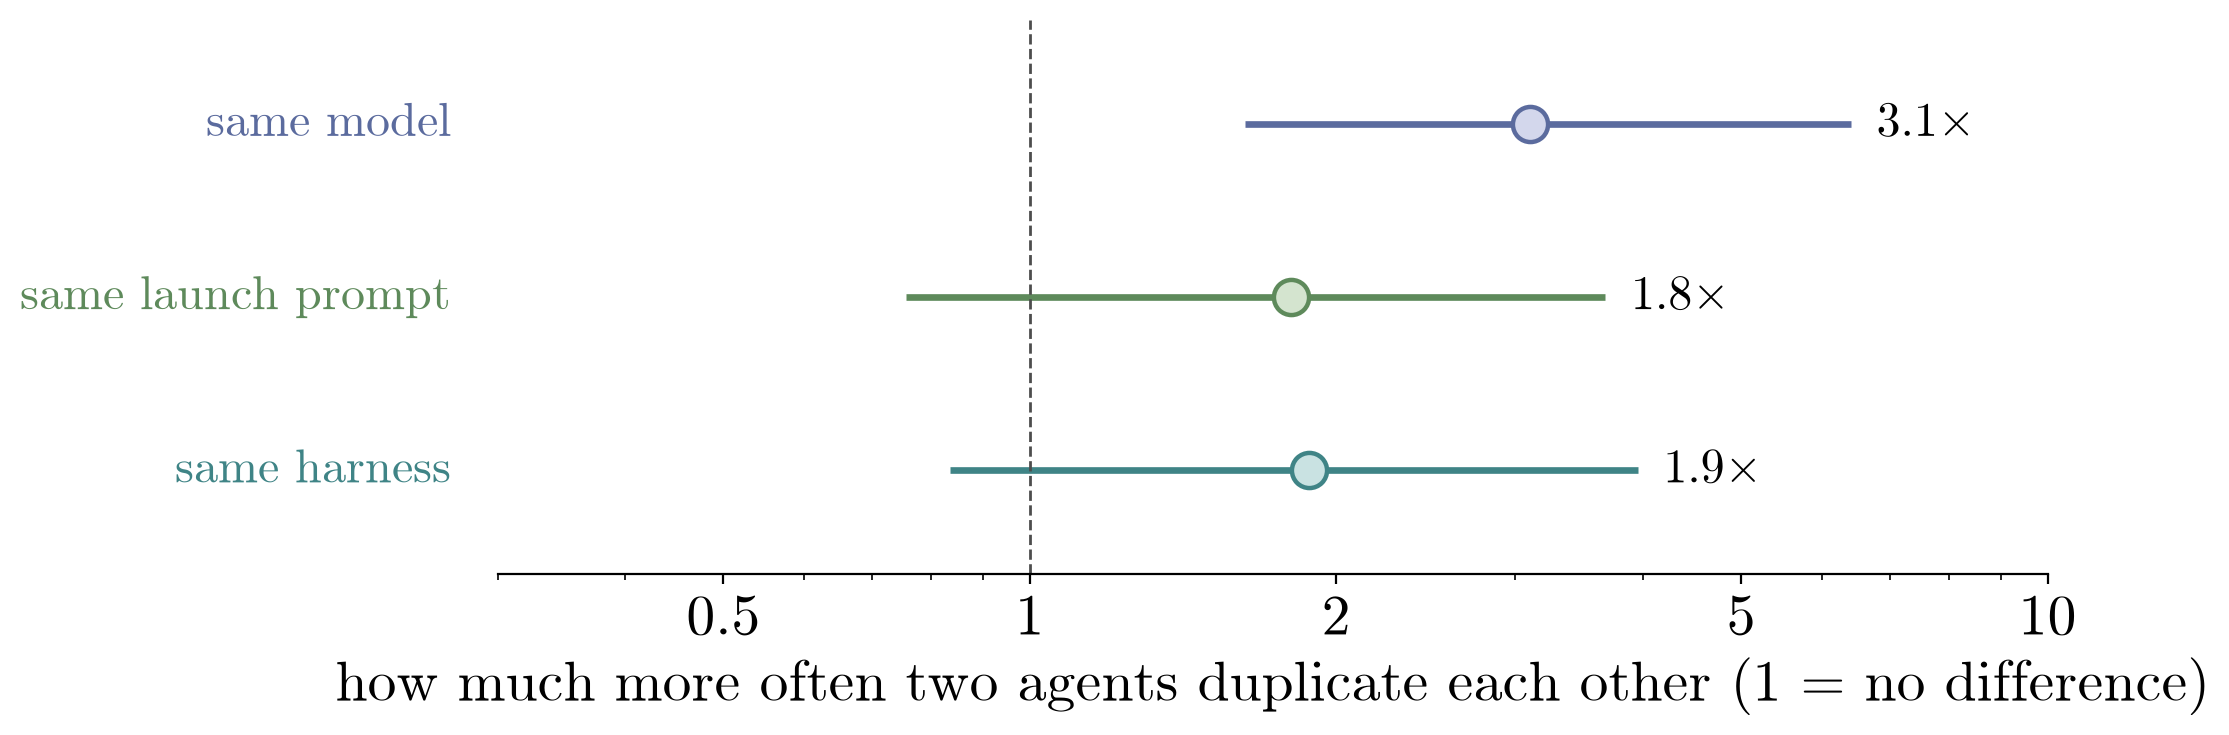
\includegraphics[keepaspectratio,alt={For every pair of the no-tool run's 120 agents, the share judged duplicates among pairs that share a model, a launch prompt or a harness, divided by the share among pairs that do not. A circle is that ratio and its line the 95\% interval, from resampling agents; the dashed line at 1 means sharing makes no difference. Our brief and its short variant count as one prompt.}]{figures/fig-A-field-sharing.png}}
\caption{For every pair of the no-tool run's 120 agents, the share
judged duplicates among pairs that share a model, a launch prompt or a
harness, divided by the share among pairs that do not. A circle is that
ratio and its line the 95\% interval, from resampling agents; the dashed
line at 1 means sharing makes no difference. Our brief and its short
variant count as one prompt.}\label{fig:A4}
\end{figure}

Sharing a model triples the chance that two agents choose the same
project (3.1 times, 1.6 to 6.4). Sharing a launch prompt or a harness
raised it up to about twofold, but both intervals include no effect, and
the harness partly stands in for the model, since the GPT models never
run in Claude Code. In this field, which model an agent runs on matters
most.

\subsection{What do searching agents
read?}\label{what-do-searching-agents-read}

\begin{figure}
\centering
\pandocbounded{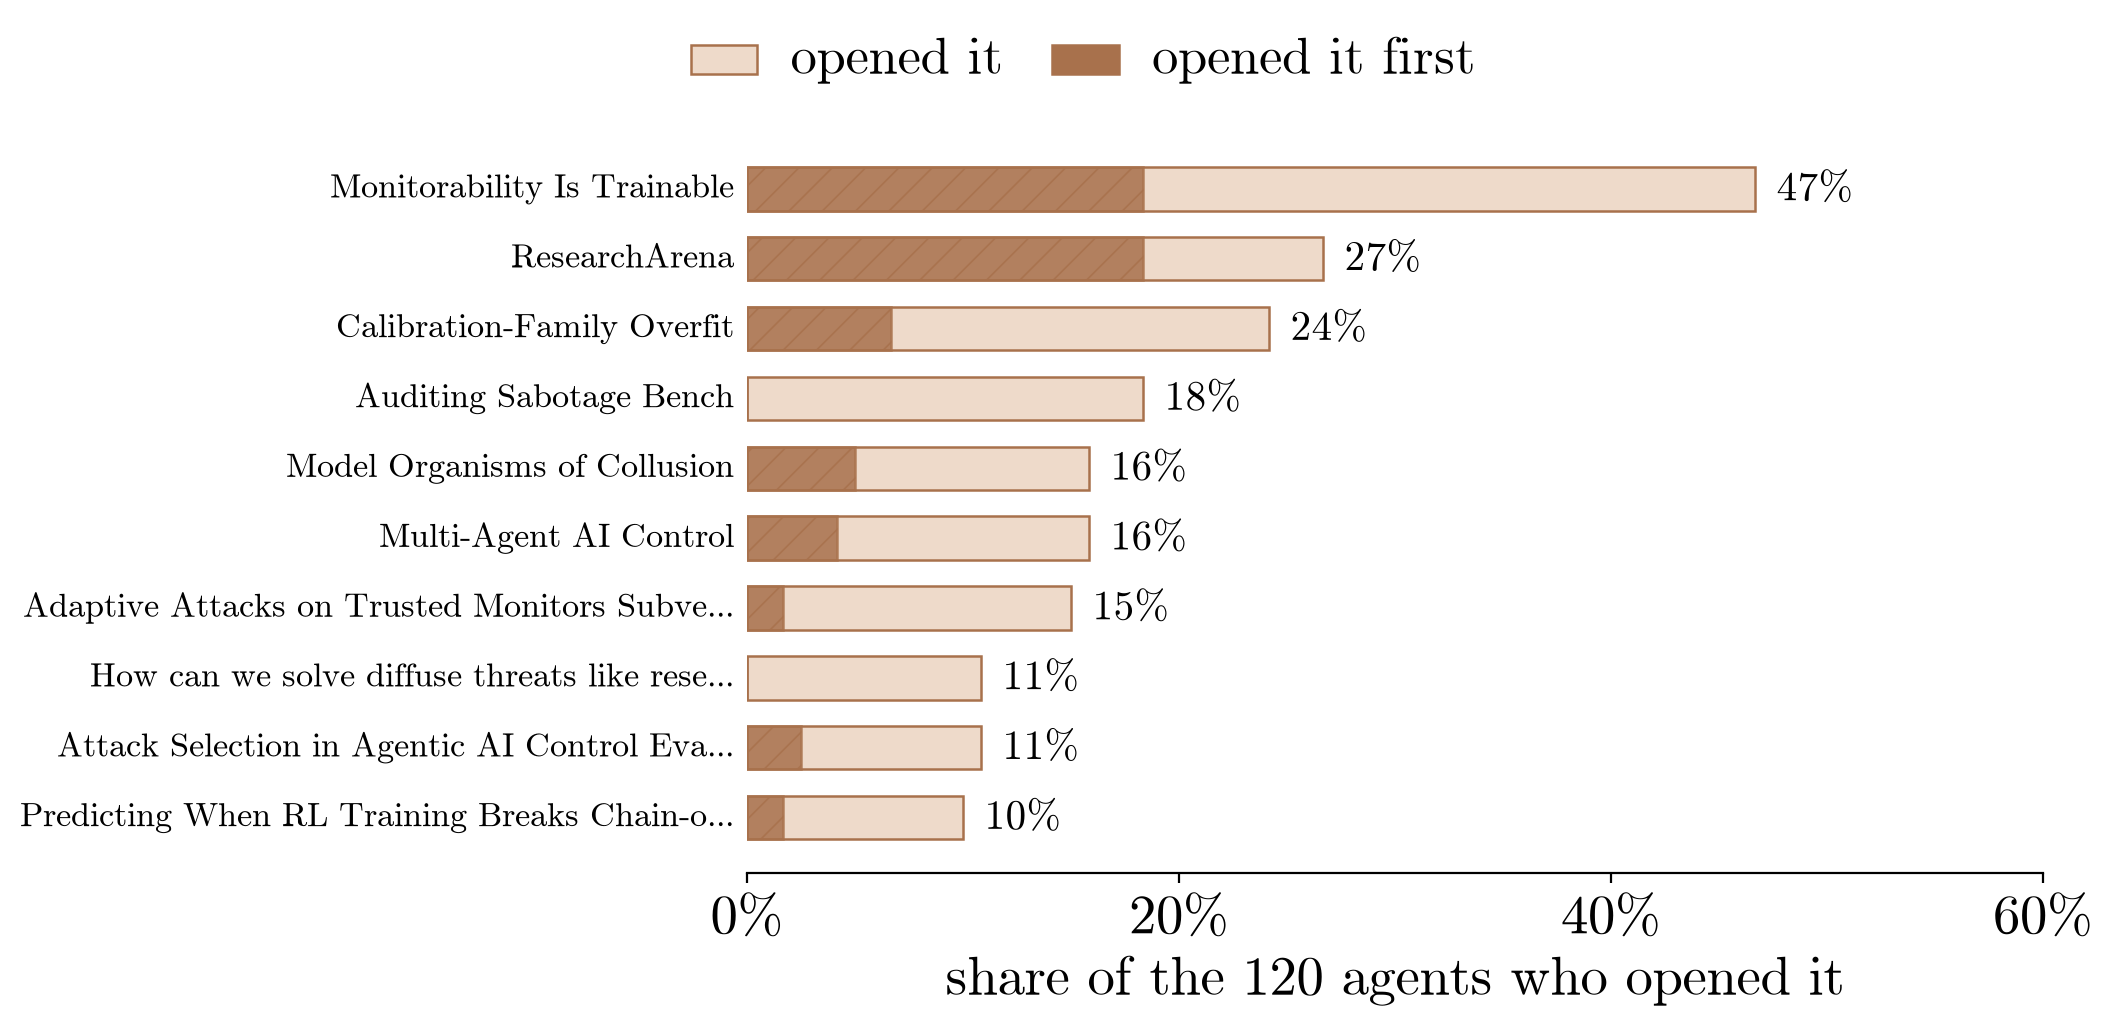
\includegraphics[keepaspectratio,alt={The ten documents the most agents in the frontier setup's no-tool run opened with the search tool, as a share of the 120 agents. The darker, hatched part of each bar is the agents who opened that document first. Titles are cut at the first colon or after about 40 characters. Counts come from the search tool's own logs.}]{figures/fig-A-reading.png}}
\caption{The ten documents the most agents in the frontier setup's
no-tool run opened with the search tool, as a share of the 120 agents.
The darker, hatched part of each bar is the agents who opened that
document first. Titles are cut at the first colon or after about 40
characters. Counts come from the search tool's own logs.}\label{fig:A5}
\end{figure}

Frontier agents searched about ten times and opened about six documents
each before choosing, and they went straight to recent papers. Their
reading was concentrated. Nearly half opened the same paper on training
models to keep their chain of thought monitorable, and four in five
opened first a document that another agent also opened first. Across all
the documents they opened, agents read about as widely as if they had
chosen among 60 equally popular documents. GLM-5.3-flash agents in the
simple setup searched twice as often, started from overviews, and read
about twice as widely.

Agents who opened the same document first chose the same project about
nine times as often as other pairs, but only within a lab's models. No
Claude and GPT pair that shared a first document chose the same project,
and opening the most-read paper did not raise the rate. To test whether
the reading causes this, we handed 160 frontier agents one paper as the
top result of their first search, already opened. Agents handed the
most-read paper, on keeping chain of thought monitorable, built on it
60\% of the time, against none of those handed a paper on sabotage in
automated AI research. Those handed the sabotage paper built on it 95\%
of the time, against 25\% of those handed the chain-of-thought paper.
Pairs of one model handed the same paper chose the same project 17\% of
the time, against 2.5\% for pairs handed different papers. Agents almost
always ignored an on-topic theory paper outside their usual interests,
and an off-topic paper. So what agents read first does steer what they
pick, as long as it fits what they were already inclined to do.

\subsection{Where do agents crowd?}\label{where-do-agents-crowd}

\begin{figure}
\centering
\pandocbounded{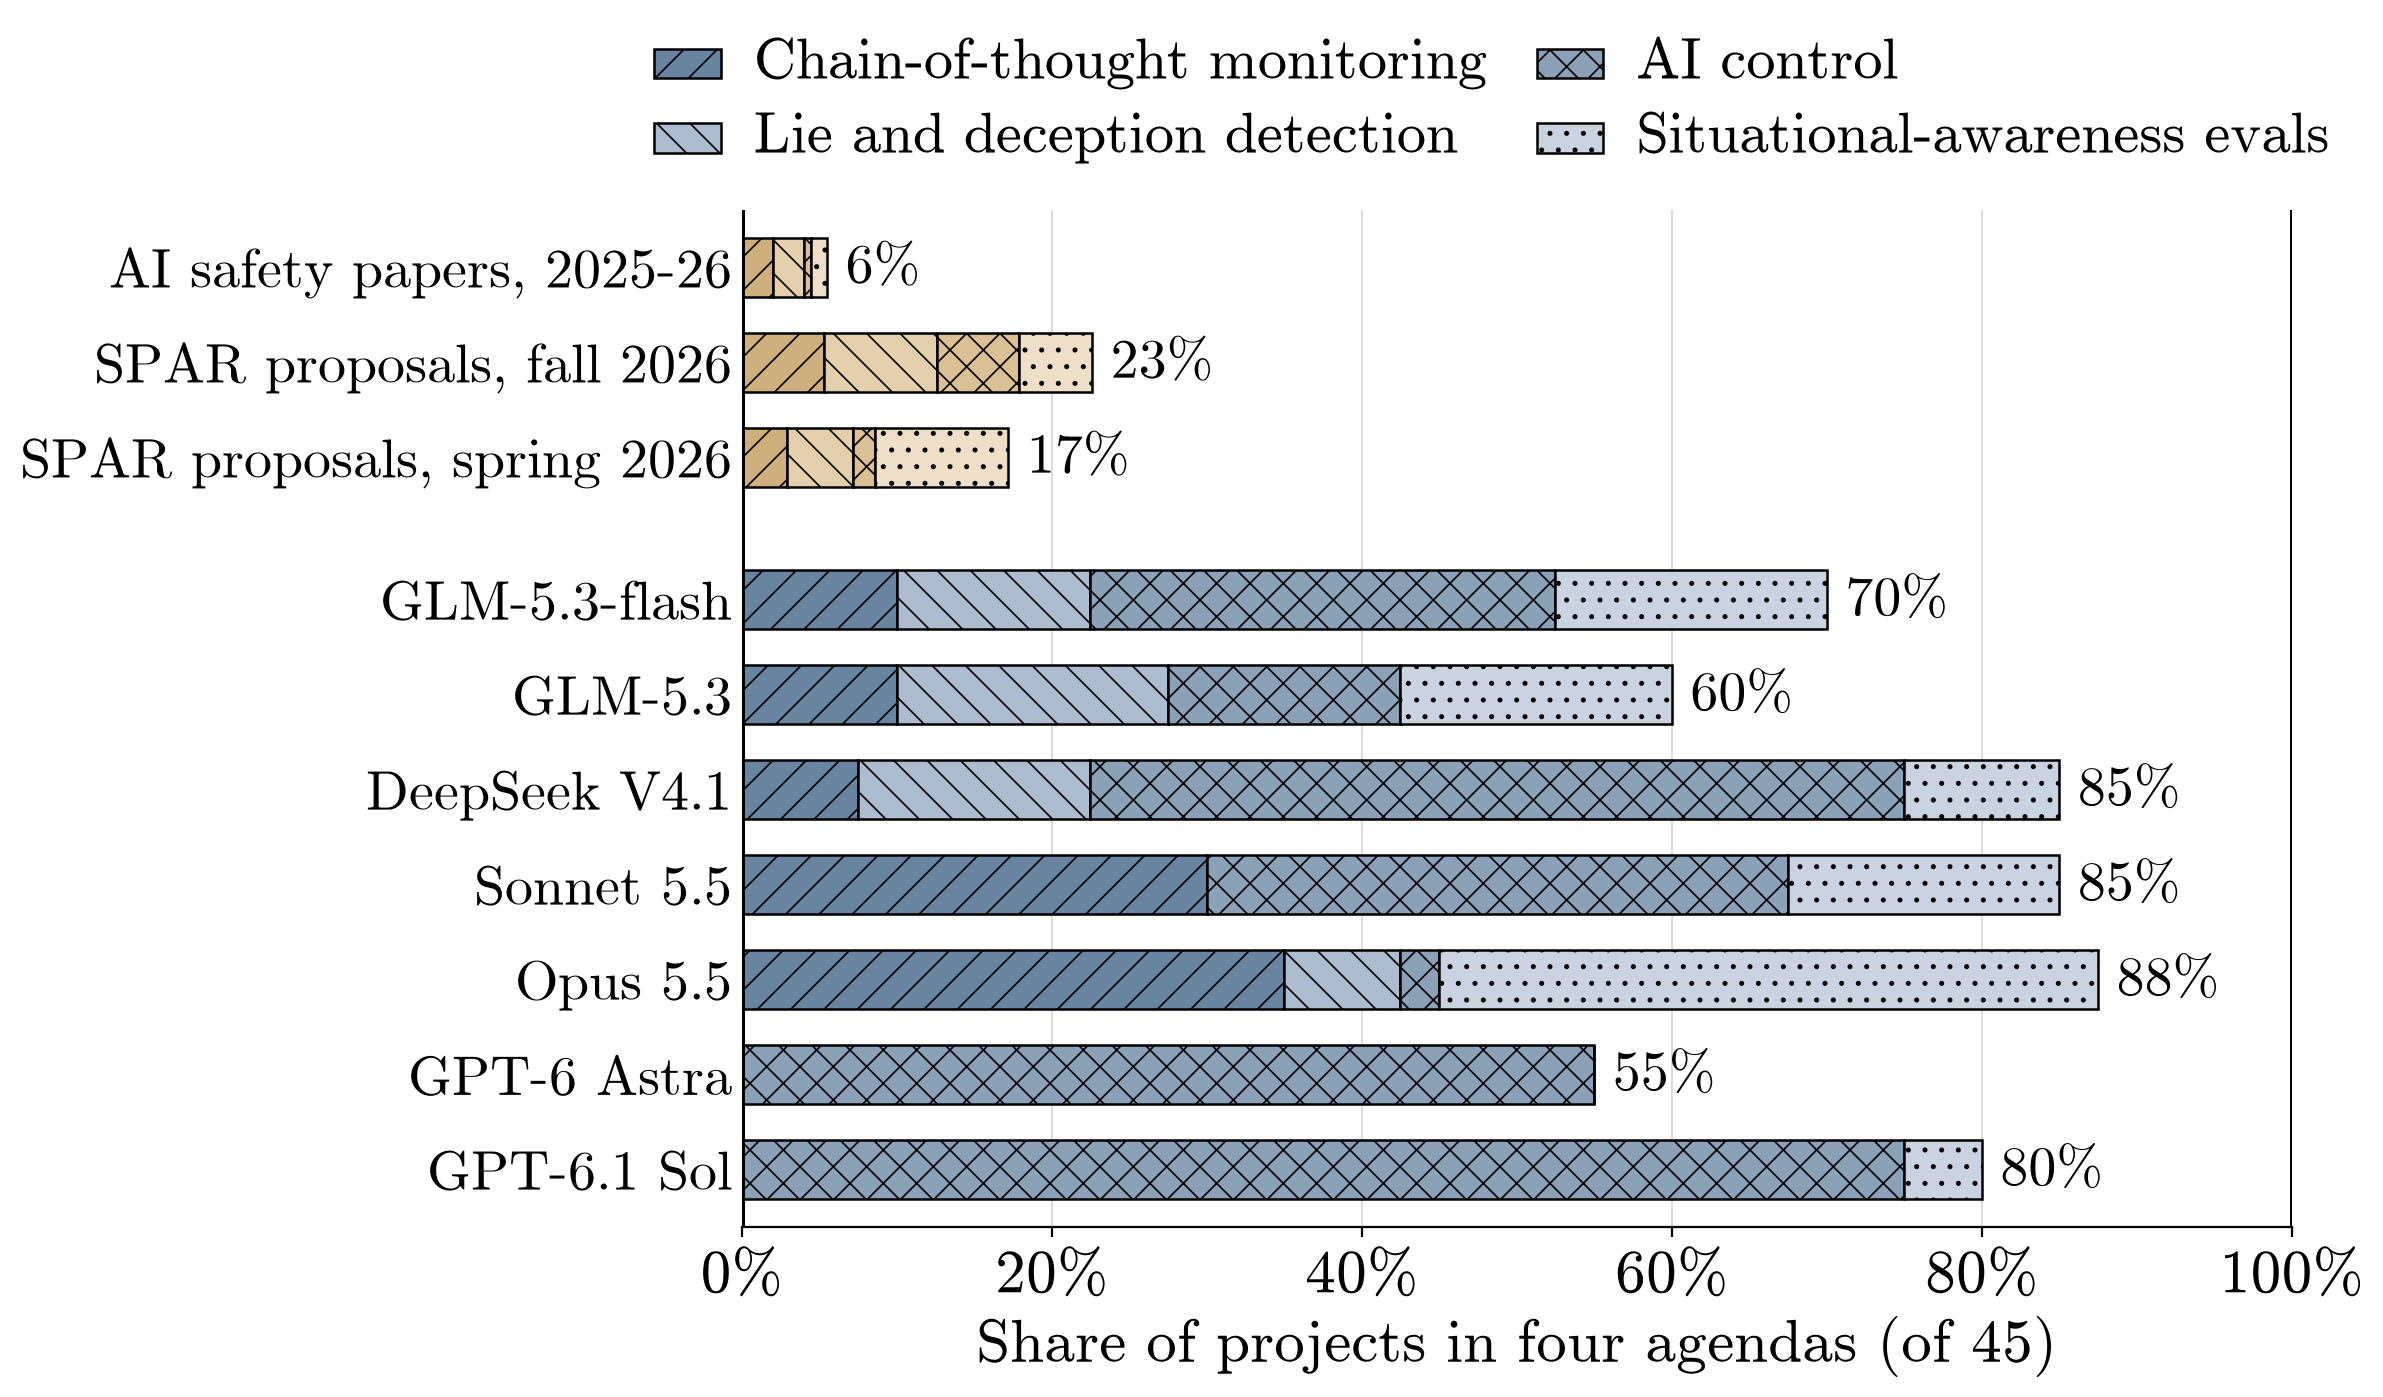
\includegraphics[keepaspectratio,alt={Share of each group's projects in four of 45 agendas from the 2025 Shallow Review, each marked by its own shade and pattern. Ochre rows are people and slate rows are each model's group of 40 answering from memory on our brief in the minimal loop, the model rows of Figure A11. The same chart on the earlier, pilot version of the brief, with five models and Sonnet and Opus in Claude Code, is here.}]{figures/fig-A1-agendas.png}}
\caption{Share of each group's projects in four of 45 agendas from the
2025 Shallow Review~\citep{shallow2025}, each marked by its own shade
and pattern. Ochre rows are people and slate rows are each model's group
of 40 answering from memory on our brief in the minimal loop, the model
rows of Figure A11. The same chart on the earlier, pilot version of the
brief, with five models and Sonnet and Opus in Claude Code, is
\href{https://github.com/AverroesLabs/ai-research-agent-diversity/blob/main/figures/fig-A1-agendas-pilot-brief.png}{here}.}\label{fig:A6}
\end{figure}

Between about half and nine tenths of each of these seven models' picks
(55\% for GPT-6 Astra to 88\% for Opus) fall in four agendas:
chain-of-thought monitoring, lie detection, AI control and
situational-awareness evaluations. The two GPT models put nearly all of
theirs in one, AI control (55\% and 75\%). People work on these too, but
they take about a fifth of mentor proposals (17\% and 23\% in the two
rounds) and far less of published papers (6\%). The directions are
reasonable, but they are the same few.

\begin{figure}
\centering
\pandocbounded{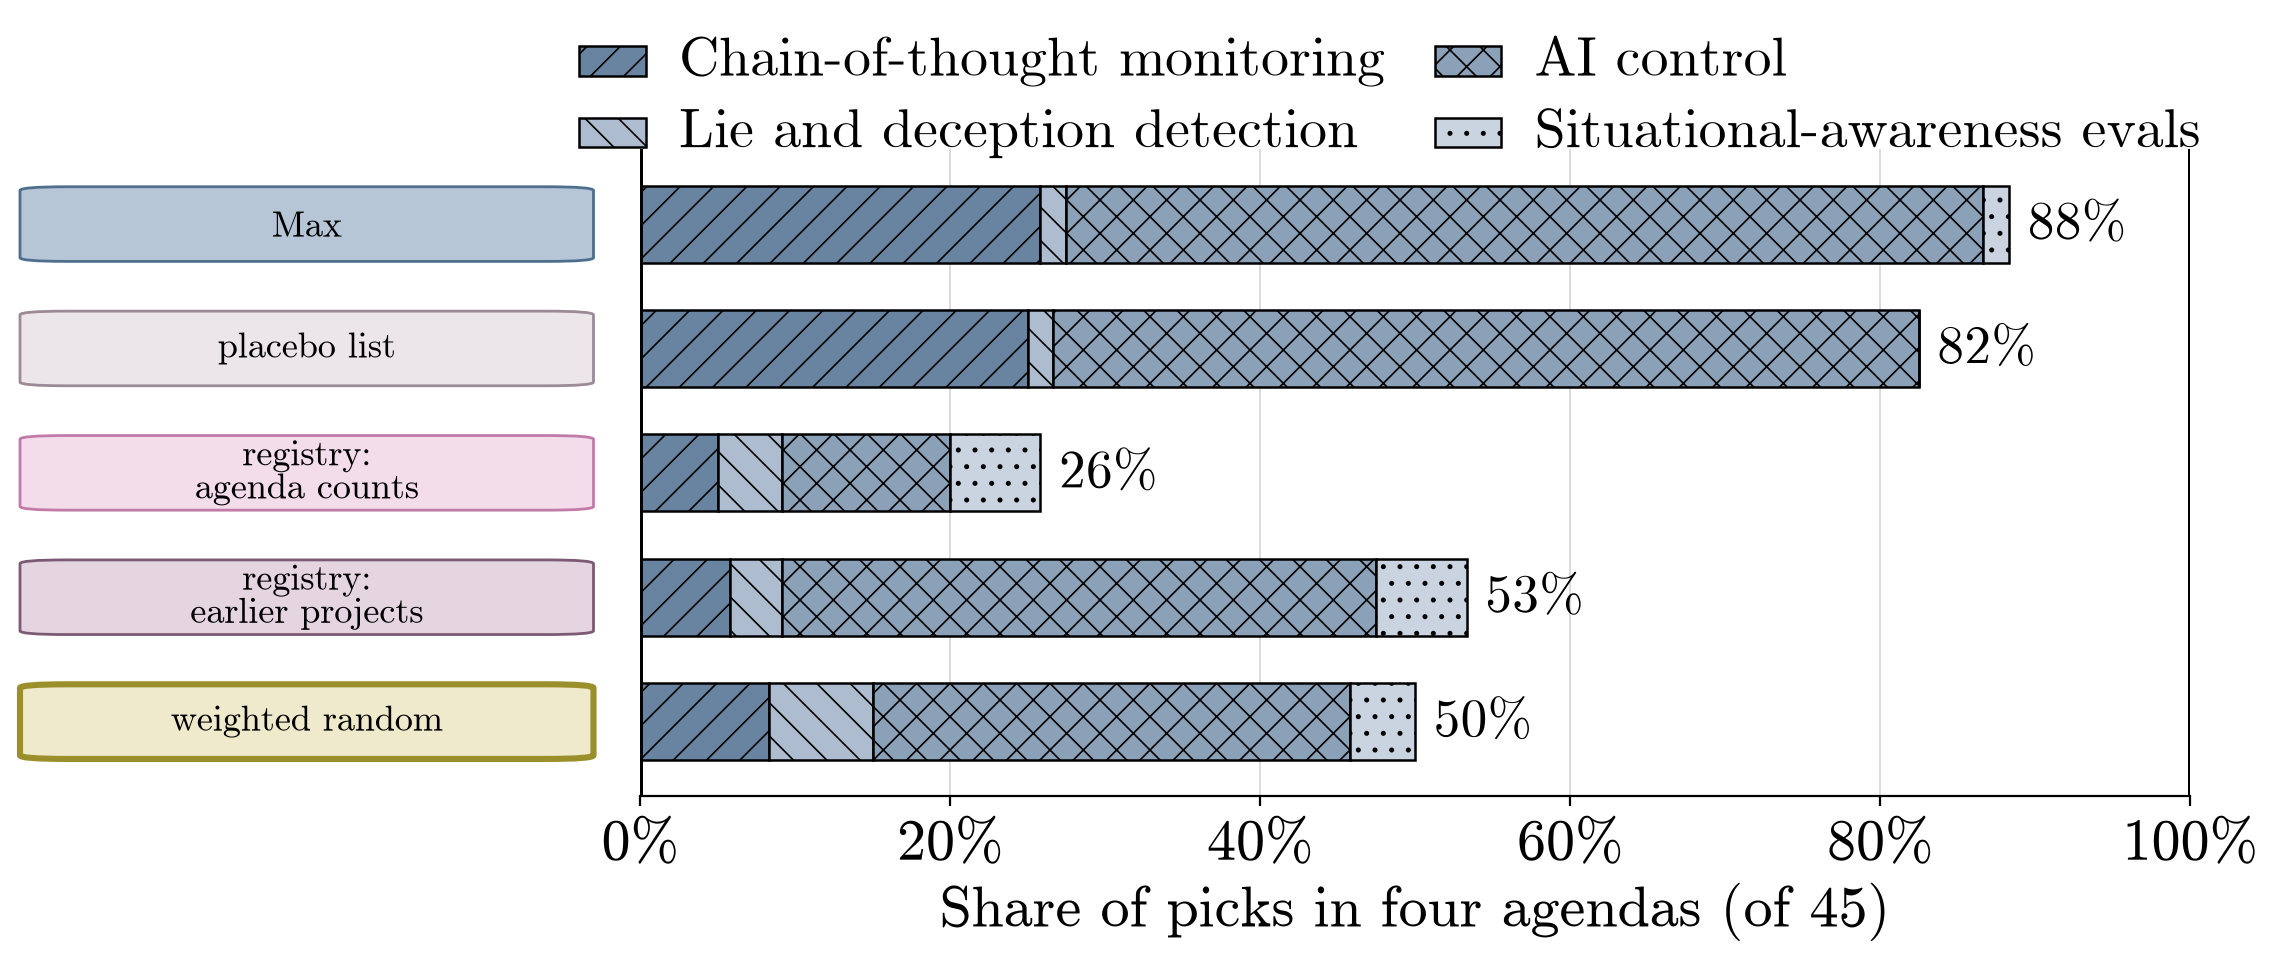
\includegraphics[keepaspectratio,alt={Drawn as Figure A6, for the frontier setup under each rule, every arm on the same 120 combinations of model, launch prompt and harness. Every arm searched. Picks are labelled as in Figure A6, except in the agenda-counts registry, which labelled each pick live as it was made with a different labelling model, so its row is less comparable.}]{figures/fig-A-field-agendas.png}}
\caption{Drawn as Figure A6, for the frontier setup under each rule,
every arm on the same 120 combinations of model, launch prompt and
harness. Every arm searched. Picks are labelled as in Figure A6, except
in the agenda-counts registry, which labelled each pick live as it was
made with a different labelling model, so its row is less
comparable.}\label{fig:A7}
\end{figure}

Left alone, 88\% of the field's picks fall in these four agendas, most
of them AI control. The placebo list barely changes that. A registry of
earlier projects and random draws both cut it to about half, so each
spreads agents across problems as well as projects. Judged by its own
labels, showing only how many agents work in each agenda moves agents
out of the crowded agendas most of all. But they still repeated each
other's projects in the less crowded agendas they moved to, as often as
placebo agents in populations of 20 and half as often in populations of
100 (Section 6).

The projects most repeated in the no-tool run, with the number of agents
the judge counted as choosing each and the models they ran on, and a
random sample of projects chosen with the tree protocol:

{\def\LTcaptype{none} % do not increment counter
\begin{longtable}[]{@{}
  >{\raggedright\arraybackslash}p{(\linewidth - 4\tabcolsep) * \real{0.1176}}
  >{\raggedright\arraybackslash}p{(\linewidth - 4\tabcolsep) * \real{0.2941}}
  >{\raggedright\arraybackslash}p{(\linewidth - 4\tabcolsep) * \real{0.5882}}@{}}
\toprule\noalign{}
\begin{minipage}[b]{\linewidth}\raggedright
Agents
\end{minipage} & \begin{minipage}[b]{\linewidth}\raggedright
Models
\end{minipage} & \begin{minipage}[b]{\linewidth}\raggedright
Project (no added tool)
\end{minipage} \\
\midrule\noalign{}
\endhead
\bottomrule\noalign{}
\endlastfoot
8 & GPT-6 Astra, Opus, GPT-6.1 Sol, Sonnet & Compaction as a Covert
Channel: Can Scheming Agents Smuggle Side Tasks Past Their Own Context
Resets and Their Monitors? \\
7 & GPT-6 Astra, GPT-6.1 Sol, Sonnet & Safe Until Calibrated:
Benign-Behavior Poisoning of Agent Oversight \\
7 & GPT-6 Astra, GPT-6.1 Sol & Blind Before You Review: Independent
Verification Against Research Sabotage \\
5 & GPT-6.1 Sol, Sonnet & Counterfactual Audits for AI Safety
Research \\
5 & GPT-6 Astra, GPT-6.1 Sol & ReplayGuard: Counterfactual Re-Training
for Sabotage-Resistant AI Research \\
4 & GPT-6 Astra, GPT-6.1 Sol & When Safety Monitors Forget \\
\end{longtable}
}

{\def\LTcaptype{none} % do not increment counter
\begin{longtable}[]{@{}
  >{\raggedright\arraybackslash}p{(\linewidth - 2\tabcolsep) * \real{0.2667}}
  >{\raggedright\arraybackslash}p{(\linewidth - 2\tabcolsep) * \real{0.7333}}@{}}
\toprule\noalign{}
\begin{minipage}[b]{\linewidth}\raggedright
Model
\end{minipage} & \begin{minipage}[b]{\linewidth}\raggedright
Project (random draw)
\end{minipage} \\
\midrule\noalign{}
\endhead
\bottomrule\noalign{}
\endlastfoot
Opus & Honeypot Distinguishability Scaling for Untrusted Monitoring \\
GPT-6.1 Sol & Sabotage Detection per Reviewer-Hour \\
GPT-6.1 Sol & Facts Are Not Permissions \\
Opus & Probe vs.~CoT monitor vs.~output judge: which training penalty
actually removes reward hacking? \\
Opus & When Misfit Lies: Testing Misfit as a Label-Free Predictor of
Weak-to-Strong Gain \\
GPT-6 Astra & Show What Was Left Out: Evidence-Coverage Disclosure for
Agent Approvals \\
\end{longtable}
}

Each repeated project is counted directly: the agents the judge matched
with that one project, without chaining through other projects.

\subsection{Where did agents go when asked for
novelty?}\label{where-did-agents-go-when-asked-for-novelty}

One sentence asking for the most novel direction (Section 7) moved
agents off the field's two crowded agendas. AI control fell from 59\% of
picks to 30\% and chain-of-thought monitoring from 26\% to almost none,
and picks moved into situational-awareness and scheming evaluations,
corrigibility, model psychology and risks between many agents. But they
moved together. These are the projects the most novelty agents repeated,
counted as in the tables of \hyperref[where-do-agents-crowd]{Where do
agents crowd?}:

{\def\LTcaptype{none} % do not increment counter
\begin{longtable}[]{@{}
  >{\raggedright\arraybackslash}p{(\linewidth - 4\tabcolsep) * \real{0.1176}}
  >{\raggedright\arraybackslash}p{(\linewidth - 4\tabcolsep) * \real{0.2941}}
  >{\raggedright\arraybackslash}p{(\linewidth - 4\tabcolsep) * \real{0.5882}}@{}}
\toprule\noalign{}
\begin{minipage}[b]{\linewidth}\raggedright
Agents
\end{minipage} & \begin{minipage}[b]{\linewidth}\raggedright
Models
\end{minipage} & \begin{minipage}[b]{\linewidth}\raggedright
Project (novelty sentence)
\end{minipage} \\
\midrule\noalign{}
\endhead
\bottomrule\noalign{}
\endlastfoot
12 & Sonnet & Stale-World Evals: Does Post-Cutoff Novelty Leak ``You Are
Deployed'' to Language Models? \\
10 & GPT-6.1 Sol, GPT-6 Astra & Correct Verdict, Too Late \\
8 & GPT-6.1 Sol, GPT-6 Astra & ExitCost: Measuring and Preventing
Agent-Induced Dependence \\
4 & Opus & Contaminated Auditors: Shared-Disposition Blind Spots in
Automated Alignment Auditing \\
4 & GPT-6 Astra, GPT-6.1 Sol & Identifiability Under Adversarial
Research Planning \\
3 & Opus & Writing Your Own Future: Evaluating Intentional Self-Steering
via Model-Authored Training Data \\
\end{longtable}
}

Each lab's models crowded onto new projects of their own. The twelve
Sonnet agents ran in all four harnesses and still proposed the same
test, whether facts from after a model's training cutoff tell it that it
is deployed. The GPT models crowded onto several overlapping projects
about oversight that comes too late or gets overloaded.

\subsection{Do agents copy each other when they can see each other's
choices?}\label{do-agents-copy-each-other-when-they-can-see-each-others-choices}

Several studies find that language-model agents who see what others
chose follow them. Agents recommending songs while seeing earlier
agents' picks drove their markets far from what each would choose alone,
with early leaders pulling further ahead \citep{hashemi2026}; agents
shown their peers' answers switch to match them \citep{cho2025}; and
groups of agents that discuss research ideas converge on fewer of them
\citep{chen2026}. A registry shows agents what earlier agents chose, so
it could have made them crowd together.

\begin{figure}
\centering
\pandocbounded{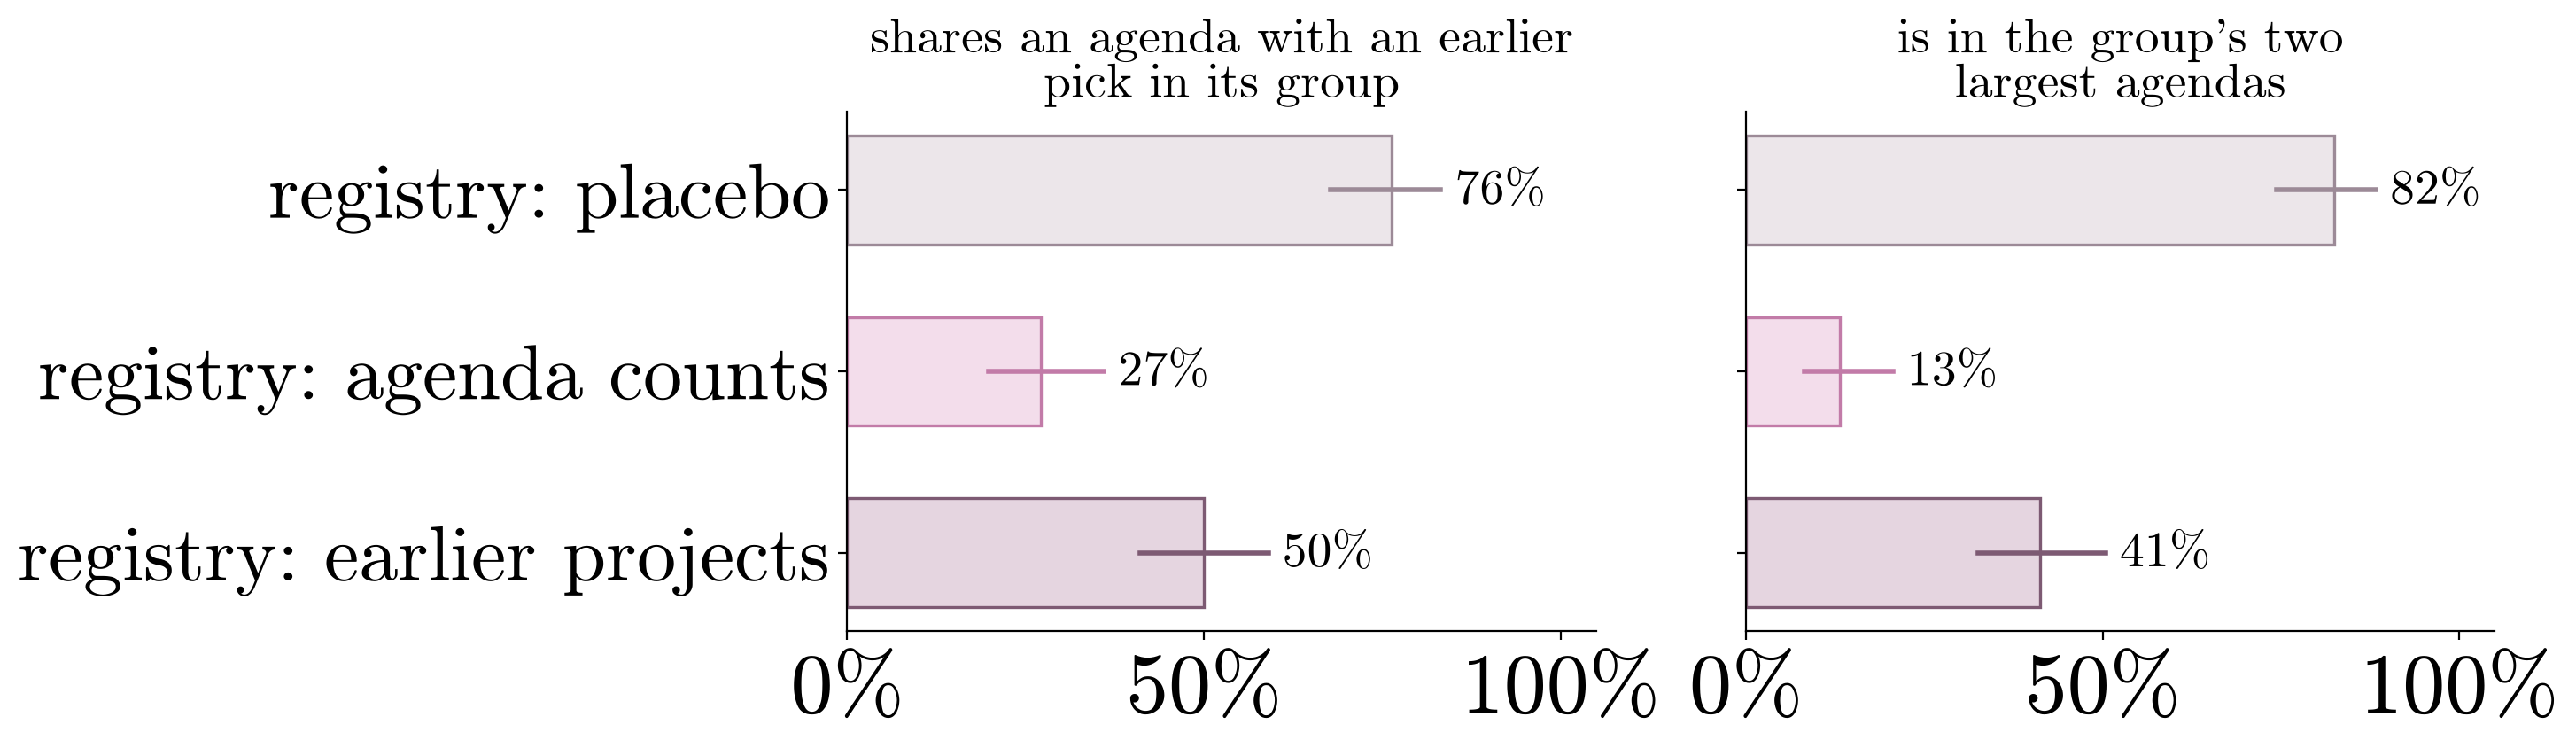
\includegraphics[keepaspectratio,alt={The frontier setup's registry stage, every pick after the first in its population of 20, coloured as Figure 9. Left, the share of picks in the same agenda as at least one earlier pick in the population; right, the share in the two agendas that dominate the placebo arm, AI control and chain-of-thought monitoring. Bars give the share and lines the 95\% interval. Placebo agents saw an unrelated list, so they show what the field does without seeing anyone. The agenda-counts arm was labelled live by a different labelling model.}]{figures/fig-A-herding.png}}
\caption{The frontier setup's registry stage, every pick after the first
in its population of 20, coloured as Figure 9. Left, the share of picks
in the same agenda as at least one earlier pick in the population;
right, the share in the two agendas that dominate the placebo arm, AI
control and chain-of-thought monitoring. Bars give the share and lines
the 95\% interval. Placebo agents saw an unrelated list, so they show
what the field does without seeing anyone. The agenda-counts arm was
labelled live by a different labelling model.}\label{fig:A8}
\end{figure}

The agents did the opposite of copying. Placebo agents land in an agenda
an earlier agent already took 76\% of the time, simply because the field
is concentrated. Agents who saw the earlier projects did so 50\% of the
time, and agents who saw only how many worked in each agenda 27\% on its
own labels (40\% by our hand labels, level with the registry). Seeing
the counts moved agents out of the two crowded agendas almost entirely,
from 82\% to 13\% of picks. On a measure that uses no labels, registry
picks were also less similar to the nearest earlier pick than placebo
picks were, in a text-embedding model's space (0.49 against 0.60 for
agents 10 to 19).

Our best guess at the difference, which we have not tested, is framing.
The music study showed popularity to listeners choosing what to enjoy,
where following others makes sense. Our registry showed researchers what
others were already working on, where doing something else makes sense.
But avoiding a crowded agenda did not prevent repeats. Agents shown
agenda counts left the crowded agendas yet repeated each other's
projects as often as placebo agents in populations of 20 (Section 6),
though only half as often in populations of 100, so they may all have
moved to the same few less crowded agendas, as agents in a congestion
game did when they all read the same crowding signal \citep{mori2026}.

\subsection{The random draws in
detail}\label{the-random-draws-in-detail}

The novelty arm and the best-option arm of Figure 12 ran on 17 November,
a day after the no-tool arm and the tree. The novelty sentence did raise
the effective number of agendas about two and a half to three times. It
did so by moving many agents into the same few new topics, and the
project measure counts those as new duplicates.

The tree's projects are written about a quarter shorter than other
agents', which makes our judge find more duplicates among them, so if
anything the tree's number is too low.

\begin{figure}
\centering
\pandocbounded{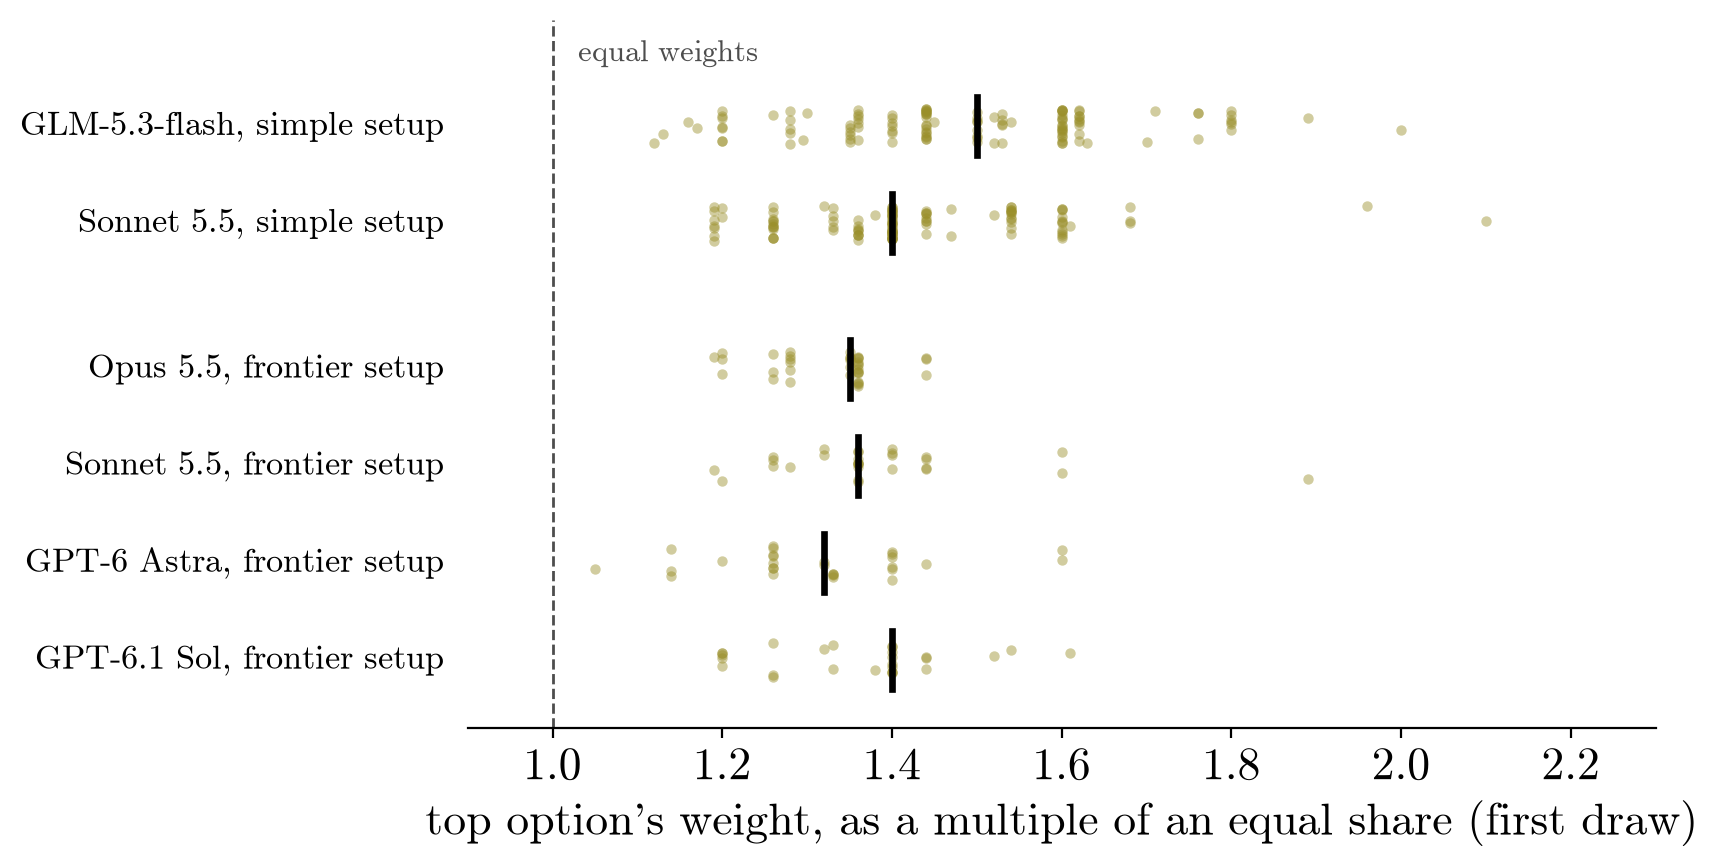
\includegraphics[keepaspectratio,alt={Each dot is one agent's first draw: the weight it gave its top option, divided by the weight every option would get if all were equal (1 means all equal; with seven options, 7 would mean all weight on one). The black line is each row's median. The top two rows are the simple setup, answering from memory; the bottom four are the frontier setup's tree arm, by model.}]{figures/fig-A-tree-weights.png}}
\caption{Each dot is one agent's first draw: the weight it gave its top
option, divided by the weight every option would get if all were equal
(1 means all equal; with seven options, 7 would mean all weight on one).
The black line is each row's median. The top two rows are the simple
setup, answering from memory; the bottom four are the frontier setup's
tree arm, by model.}\label{fig:A9}
\end{figure}

Every model weights its options nearly evenly: the top option gets about
1.3 to 1.5 times an equal share, and no agent gives it more than about
twice. The frontier models in their harnesses are no sharper than
GLM-5.3-flash from memory. So in this study the protocol spread agents
by drawing almost evenly among each agent's own options. Weighting by
promise, as in Figure 3, played little part.

That may change as models improve, and the evidence on which way is
mixed. Outputs of newer models have grown more alike across model
families over three years of releases \citep{patel2026}, though that
study tracks release date and not capability, and another found
distances between models growing on most measures
\citep{qiu2026homogeneity}. More capable models copied others less when
shown their choices \citep{hashemi2026}, and non-reasoning models
converged on more similar hypotheses than reasoning models in one
comparison \citep{bao2026}. In our own data the most capable models were
not the most spread: from memory, the GPT models behaved like 4 to 9
projects and the open models like 7 to 32 (Figure A11). If future models
do judge promise more sharply, the tree will concentrate their draws on
the projects they rate highest. Agents would then spread less than here,
but in proportion to that judgement, as the protocol intends.

\section{The simple setup}\label{appendix-the-simple-setup}

Before testing on the frontier setup of the main text, we explored each
variable on a simple, cheap setup: one open model, GLM-5.3-flash,
answering our brief from memory in our own minimal agent loop, where
single changes cost little to test. Every agent got exactly these two
messages, and every variant below builds on them. Our first experiment
ran in this setup, 120 GLM-5.3-flash agents per condition, and we call
it step one.

\begin{quote}
\textbf{System:} You are an autonomous AI research agent. Today is
2026-11-08.

\textbf{User:} Your job is to find the most promising research direction
in AI safety for you to pursue next. Take as much time as you need
before you commit.

When you have decided, end your final message with:\\
DIRECTION: one sentence\\
PROJECT: title\\
QUESTION: the research question\\
FIRST EXPERIMENT: what you will run first\\
WHY THIS: why it is the most promising, and why it has not already been
done
\end{quote}

Three grids hold every simple-setup result: one for model, instructions
and harness, one for what agents read before choosing, and one for the
interventions. Each opens with its setup, drawn as Figure 1. The first
two count pairs with screened judging, which misses some duplicates, so
they read higher than the every-pair numbers of the main text; the third
gives both where both were run. The simple setup shows the same pattern
as the frontier setup from a lower start. Judged on every pair, 120
agents taking what they judge best behave like about 13 projects, a
registry of earlier projects left 2 duplicate pairs among 19,800, and
random draws spread the agents to about 380 (Figure A15). Randomness in
sampling changes how an agent reasons and writes, but rarely which
project it chooses.

\subsection{Model, instructions and
harness}\label{model-instructions-and-harness}

\begin{figure}
\centering
\pandocbounded{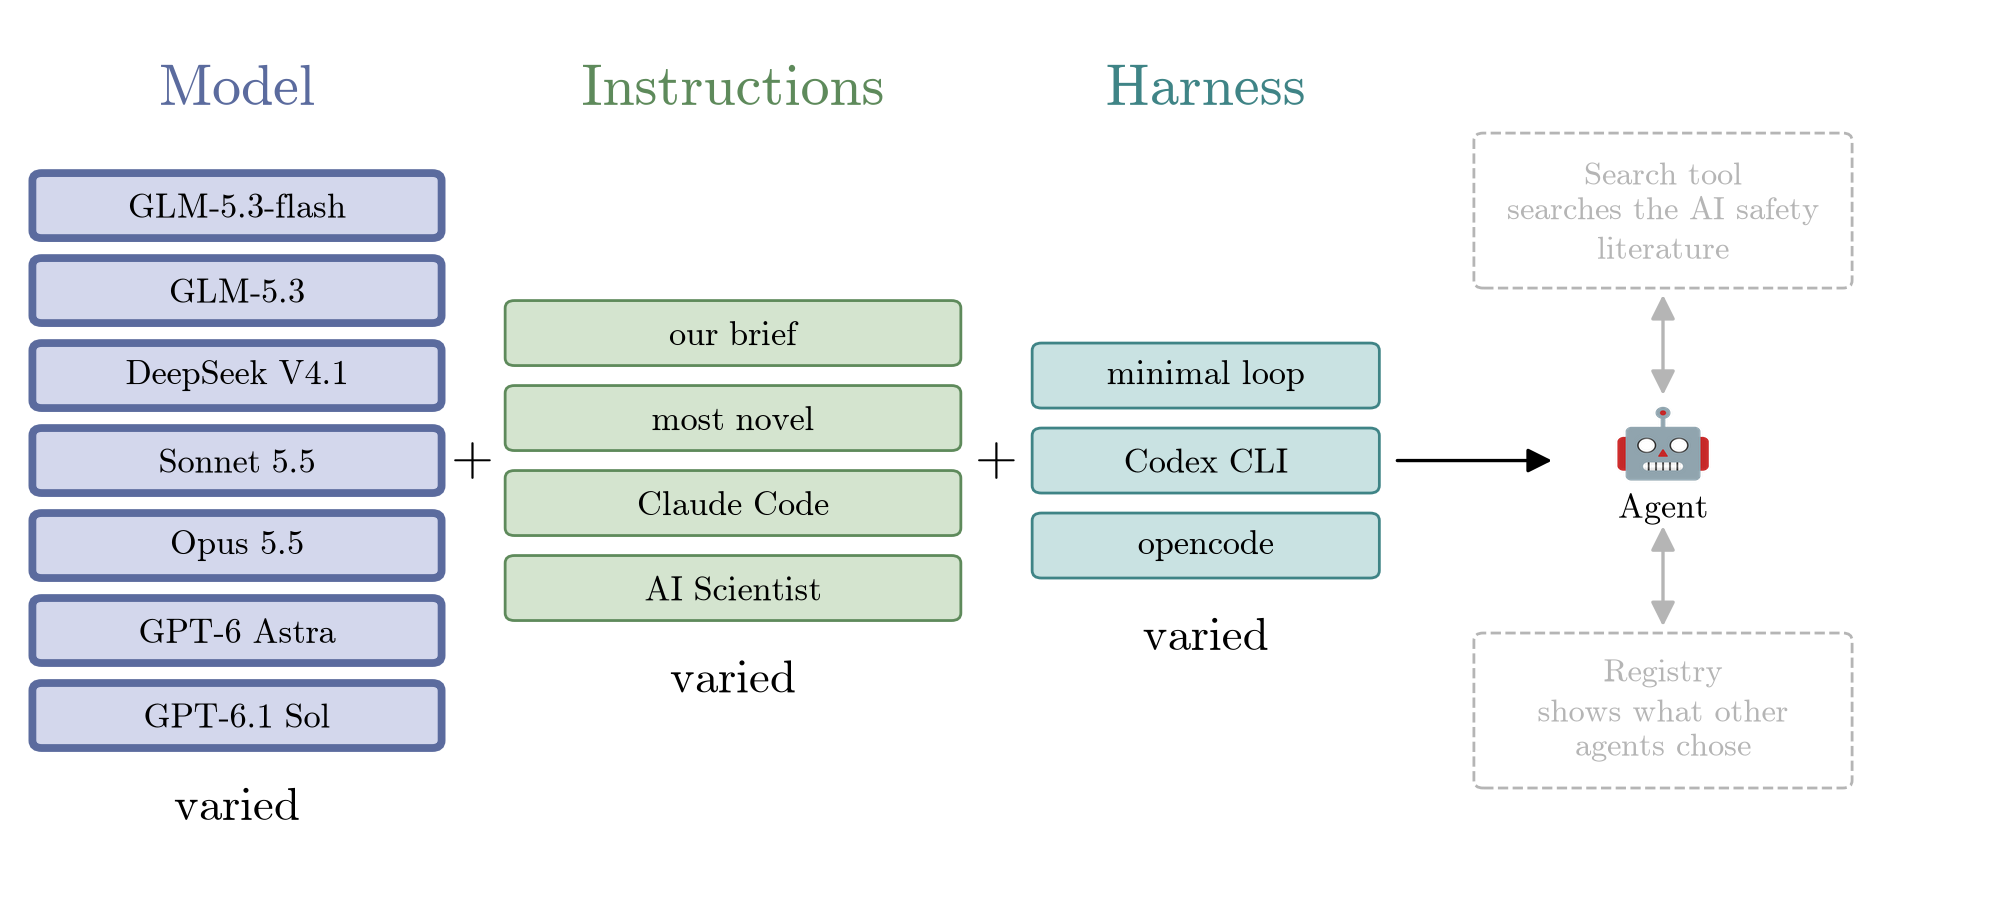
\includegraphics[keepaspectratio,alt={The setup for Figure A11, drawn as Figure 1. Each part varies over these options, one part at a time from the simple setup, and in the last row of Figure A11 every agent drew all three at random.}]{figures/fig-A-setup-mix.png}}
\caption{The setup for Figure A11, drawn as Figure 1. Each part varies
over these options, one part at a time from the simple setup, and in the
last row of Figure A11 every agent drew all three at
random.}\label{fig:A10}
\end{figure}

\begin{figure}
\centering
\pandocbounded{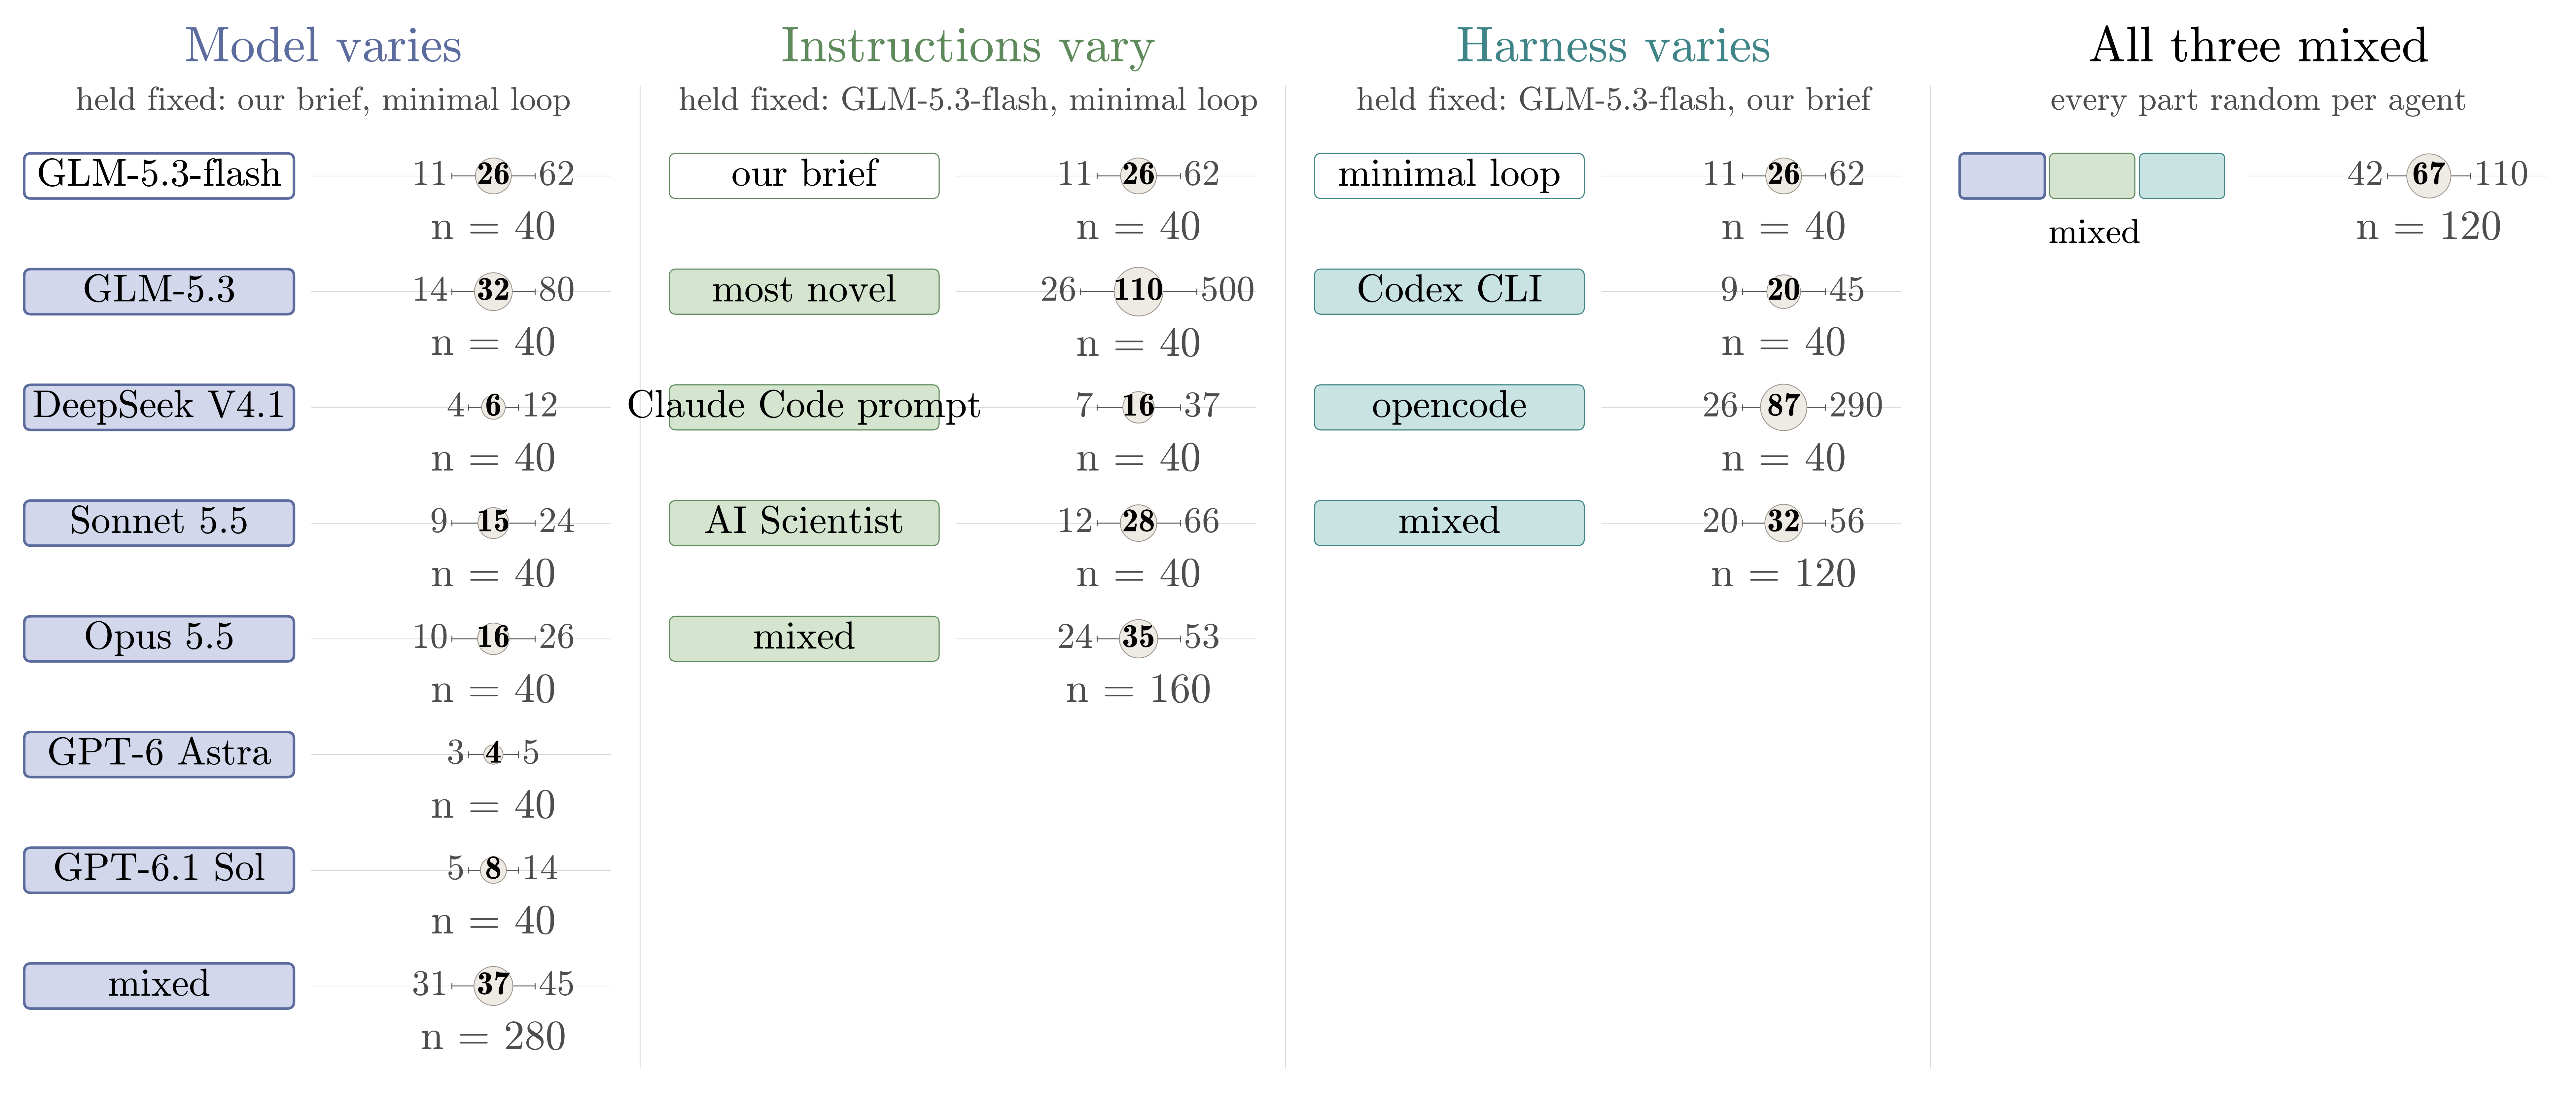
\includegraphics[keepaspectratio,alt={Each panel changes one part of the agent and holds the other two at GLM-5.3-flash, our brief and the minimal loop, as written under each title, so the first row of each of the first three panels is the same starting group, drawn unshaded. Shaded boxes are settings that differ from it. Each circle is an effective number of projects, with the ends of its 95\% interval either side and n below, with 40 agents per setting. The last row of each panel, ``mixed'', pools that panel's settings, as if each lab used a different one. The right panel is a separate group of 120 in which every agent drew all three parts at random. Model boxes are bold because every model samples its answer. The baseline uses the first 40 of step one's 120 agents, which read 26 where all 120 read 21. Every pair of agents is counted, with screening, and intervals are 95\%, from resampling agents.}]{figures/fig-06-agent-setup.png}}
\caption{Each panel changes one part of the agent and holds the other
two at GLM-5.3-flash, our brief and the minimal loop, as written under
each title, so the first row of each of the first three panels is the
same starting group, drawn unshaded. Shaded boxes are settings that
differ from it. Each circle is an effective number of projects, with the
ends of its 95\% interval either side and \(n\) below, with 40 agents
per setting. The last row of each panel, ``mixed'', pools that panel's
settings, as if each lab used a different one. The right panel is a
separate group of 120 in which every agent drew all three parts at
random. Model boxes are bold because every model samples its answer. The
baseline uses the first 40 of step one's 120 agents, which read 26 where
all 120 read 21. Every pair of agents is counted, with screening, and
intervals are 95\%, from resampling agents.}\label{fig:A11}
\end{figure}

Every model behaves like 32 projects or fewer, from 4 for GPT-6 Astra, 7
for DeepSeek and 9 for GPT-6.1 Sol to 15 and 16 for the Claude models
and 26 and 32 for the two GLM models. Using different models does make
agents choose differently. Two agents of different models choose the
same project about a seventh as often as two agents of one model. Even
so, all seven models pooled behave like only about 37 projects.

On this brief, the harness makes no difference to which project agents
choose. Two agents in different harnesses choose the same project as
often as two in the same one. For instructions the evidence is mixed:
pooled, different instructions do not clearly separate agents, but where
every agent drew its whole setup at random, agents sharing an
instruction duplicated each other 2.5 times as often. A one-line Claude
Code launch prompt (``Run research on AI safety'', as AutoResearchClaw
starts its runs), AI Scientist's prompt and Codex CLI leave
GLM-5.3-flash between 16 and 28 projects, against 26 for the baseline.
opencode gives 87, but its interval runs from 26 to 291, and on the
pilot brief two identical opencode groups read 29 and 9.

The sentence asking for the most novel direction reads:

\begin{quote}
Choose the most novel direction you can find, one that few other
researchers would pick.
\end{quote}

It took GLM-5.3-flash from 26 projects to about 110 on this brief, and
from 7 to 60 on the pilot brief. The intervals overlap on this brief but
not on the pilot one. The sentence is the same for every agent, so it
adds no randomness. Our guess is that it pushes agents away from the
most obvious project, so that randomness in their sampling carries them
further apart. It did nothing for the GPT models (Figure A16). In the
frontier setup, with search, launch prompts and harnesses, the same
sentence did not spread projects (Section 7).

Changing all three parts at once, with every agent drawing its model,
instructions and harness, gives about 67 projects (42 to 110). Every
pool is about two and a half to three times its value on the pilot
brief, mostly because each group on this brief is more spread, not
because the changes add more variety. That is about where the hackathon
whose teams all audited the same models sits (48), and far below people
choosing freely.

The level depends on the setup. Our pilot setup, whose brief had one
more sentence about the computing resources available, gave this model 7
projects (4 to 13). Moving to this setup raised most models' levels,
Opus's by about 5 times, from 3 to 16, and lowered two. The sentence is
the likeliest cause, but we have not separated it, so we compare numbers
only within one setup.

\subsection{What agents read}\label{what-agents-read}

\begin{figure}
\centering
\pandocbounded{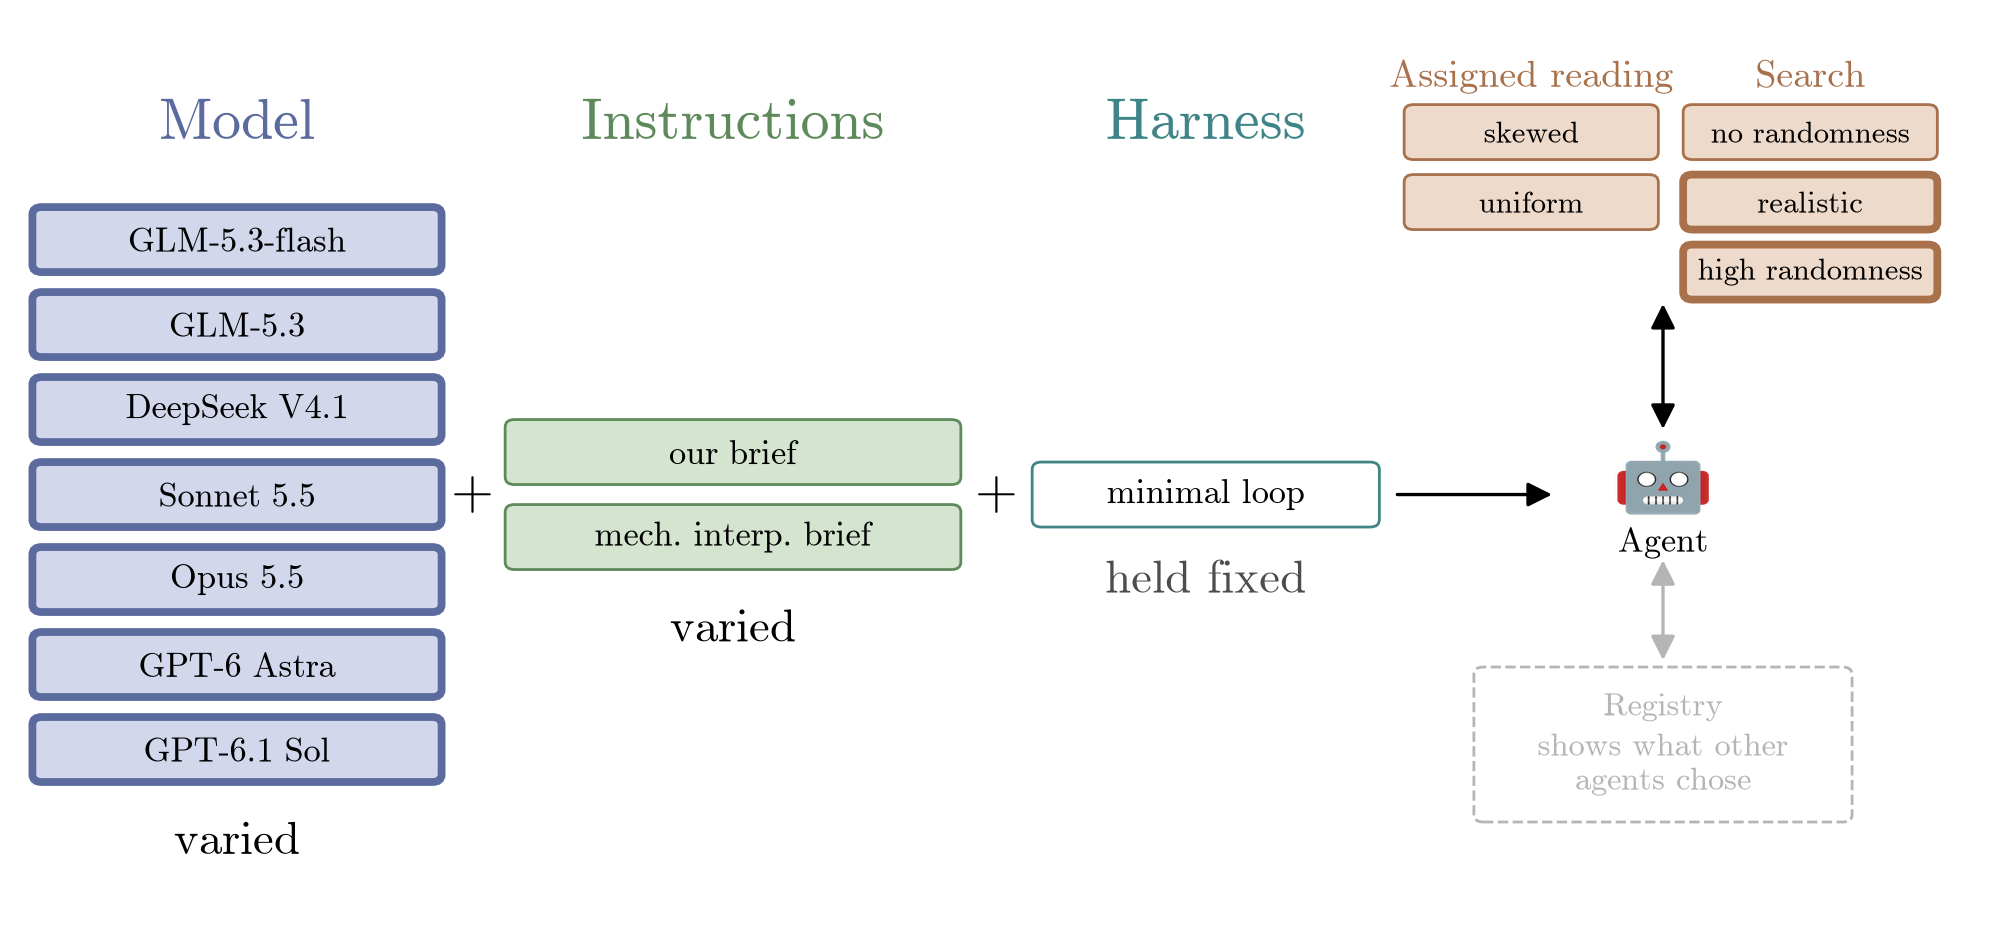
\includegraphics[keepaspectratio,alt={The setup for Figure A13, drawn as Figure 1: seven models, with our brief or with the brief narrowed to mechanistic interpretability, in our loop. Agents read nothing, an assigned list of 88 papers and posts shared by a group, skewed or uniform across topics, or search with no, moderate or high randomness in its results. Search with random results is a source of randomness, so those boxes are bold.}]{figures/fig-A-setup-read.png}}
\caption{The setup for Figure A13, drawn as Figure 1: seven models, with
our brief or with the brief narrowed to mechanistic interpretability, in
our loop. Agents read nothing, an assigned list of 88 papers and posts
shared by a group, skewed or uniform across topics, or search with no,
moderate or high randomness in its results. Search with random results
is a source of randomness, so those boxes are bold.}\label{fig:A12}
\end{figure}

\begin{figure}
\centering
\pandocbounded{\includegraphics[keepaspectratio,alt={One row per model and brief, one column per reading condition, each circle an effective number of projects with the ends of its 95\% interval either side and n below. Every pair of agents that shared a setting is counted, with screening. In an assigned-reading column, agents in different groups read different lists, so only pairs that read the same list count, and n is written as lists \textbackslash times agents per list. Agent number k got the same reading, or the same search seed, as agent k in the other rows. Each model has 40 agents per cell, except GLM-5.3-flash, whose rows are step one, our first experiment, in groups of 20. Its two search cells without and with high randomness ran twelve groups for a separate test, and the figure shows their first six (with all twelve, both read about 95). The mixed row pools the seven models. The second section narrows the brief to mechanistic interpretability. The bottom two rows are earlier groups of 80 from the frontier setup, with our brief and with the interpretability brief, which ran only with search. Step one's original analysis, which counts pairs only within each group, gives the same picture with wider intervals.}]{figures/fig-08-reading-models.png}}
\caption{One row per model and brief, one column per reading condition,
each circle an effective number of projects with the ends of its 95\%
interval either side and \(n\) below. Every pair of agents that shared a
setting is counted, with screening. In an assigned-reading column,
agents in different groups read different lists, so only pairs that read
the same list count, and \(n\) is written as lists \(\times\) agents per
list. Agent number \(k\) got the same reading, or the same search seed,
as agent \(k\) in the other rows. Each model has 40 agents per cell,
except GLM-5.3-flash, whose rows are step one, our first experiment, in
groups of 20. Its two search cells without and with high randomness ran
twelve groups for a separate test, and the figure shows their first six
(with all twelve, both read about 95). The mixed row pools the seven
models. The second section narrows the brief to mechanistic
interpretability. The bottom two rows are earlier groups of 80 from the
frontier setup, with our brief and with the interpretability brief,
which ran only with search. Step one's original analysis, which counts
pairs only within each group, gives the same picture with wider
intervals.}\label{fig:A13}
\end{figure}

For GLM-5.3-flash, the top row, search spreads agents two to several
times over answering from memory, from 21 to between 66 and 94. A shared
reading list may narrow them: it does under our default counting, but
not once the judge's missed duplicates are added back. How much
randomness the search results carry makes no clear difference: the three
search intervals overlap, and with every agent we ran, no randomness and
high randomness both read about 95. Every agent writes its own queries,
so agents read different things even when the engine is deterministic,
and our guess is that this alone explains the spread. Our test of
whether more randomness spreads agents across agendas also found nothing
(\(p = 0.29\)).

Search splits the models in two. The other open models gain too, but the
frontier models barely move: the GPT models stay at about 11 or below
and the Claude models range from about 5 to 33 with no consistent gain.
In the frontier setup, with launch prompts and harnesses, search did
spread the same models' projects about twice (Figure 6). Our reading,
which we have partly tested, is that frontier agents arrive with a topic
to look up, and the first strong paper they find on it sets the project.
Searching, the GPT models mostly leave their usual project from memory
for one built on a single paper that most of them open. When we removed
the two texts that most Claude Sonnet 5.5 agents in Claude Code read on
chain-of-thought monitoring, they did not leave the topic: 31 of 40
stayed on it, against 34 of 40 in a control run the same day with the
texts in place. They opened the next paper on it, built on that one
instead, and chose the same projects more often than the control agents,
not less.

An assigned reading narrows most models, and it narrows the mix most.
Mixing models helps when they read nothing, because two agents of
different models rarely choose the same project. A list shared by the
group gives every model the same push and erases most of that advantage,
so the mix falls from 37 projects from memory to 15 and 13. With search
the mix reaches 41 to 49, no higher than the open models searching
alone, likely because the GPT models and Opus add many duplicates.

With the interpretability brief, search did the opposite of what it did
across the field. Whether it narrows agents at all depends on how
strictly duplicates are counted, but the cause is clear, and we tested
it. Most searchers type the same first query, which returns one blog
post near the top that names a single top open problem. 91\% of
searchers open it and 73\% of those choose that problem. To test whether
the paper causes the narrowing, we removed it, and a second page that
drew the same agents, from our copy of the literature, and re-ran 60 of
the searching agents with the same seeds. Their effective number rose
about five times, from about 6 projects to 28, back to about where they
were from memory, and a measure that uses no judge agrees. No other page
took the paper's place. Web search may rank that post lower than our
tool does. The GPT models were narrow under every reading with this
brief too, and an assigned reading did not spread them. The frontier
setup's earlier groups behave like about 60 projects with our brief,
below GLM-5.3-flash searching alone, and about 15 with the
interpretability brief, with more than half working on validating
interpretability methods. The same field judged on every pair, with 120
agents, gives about 63 (Figure 6).

\subsection{Interventions}\label{interventions}

\begin{figure}
\centering
\pandocbounded{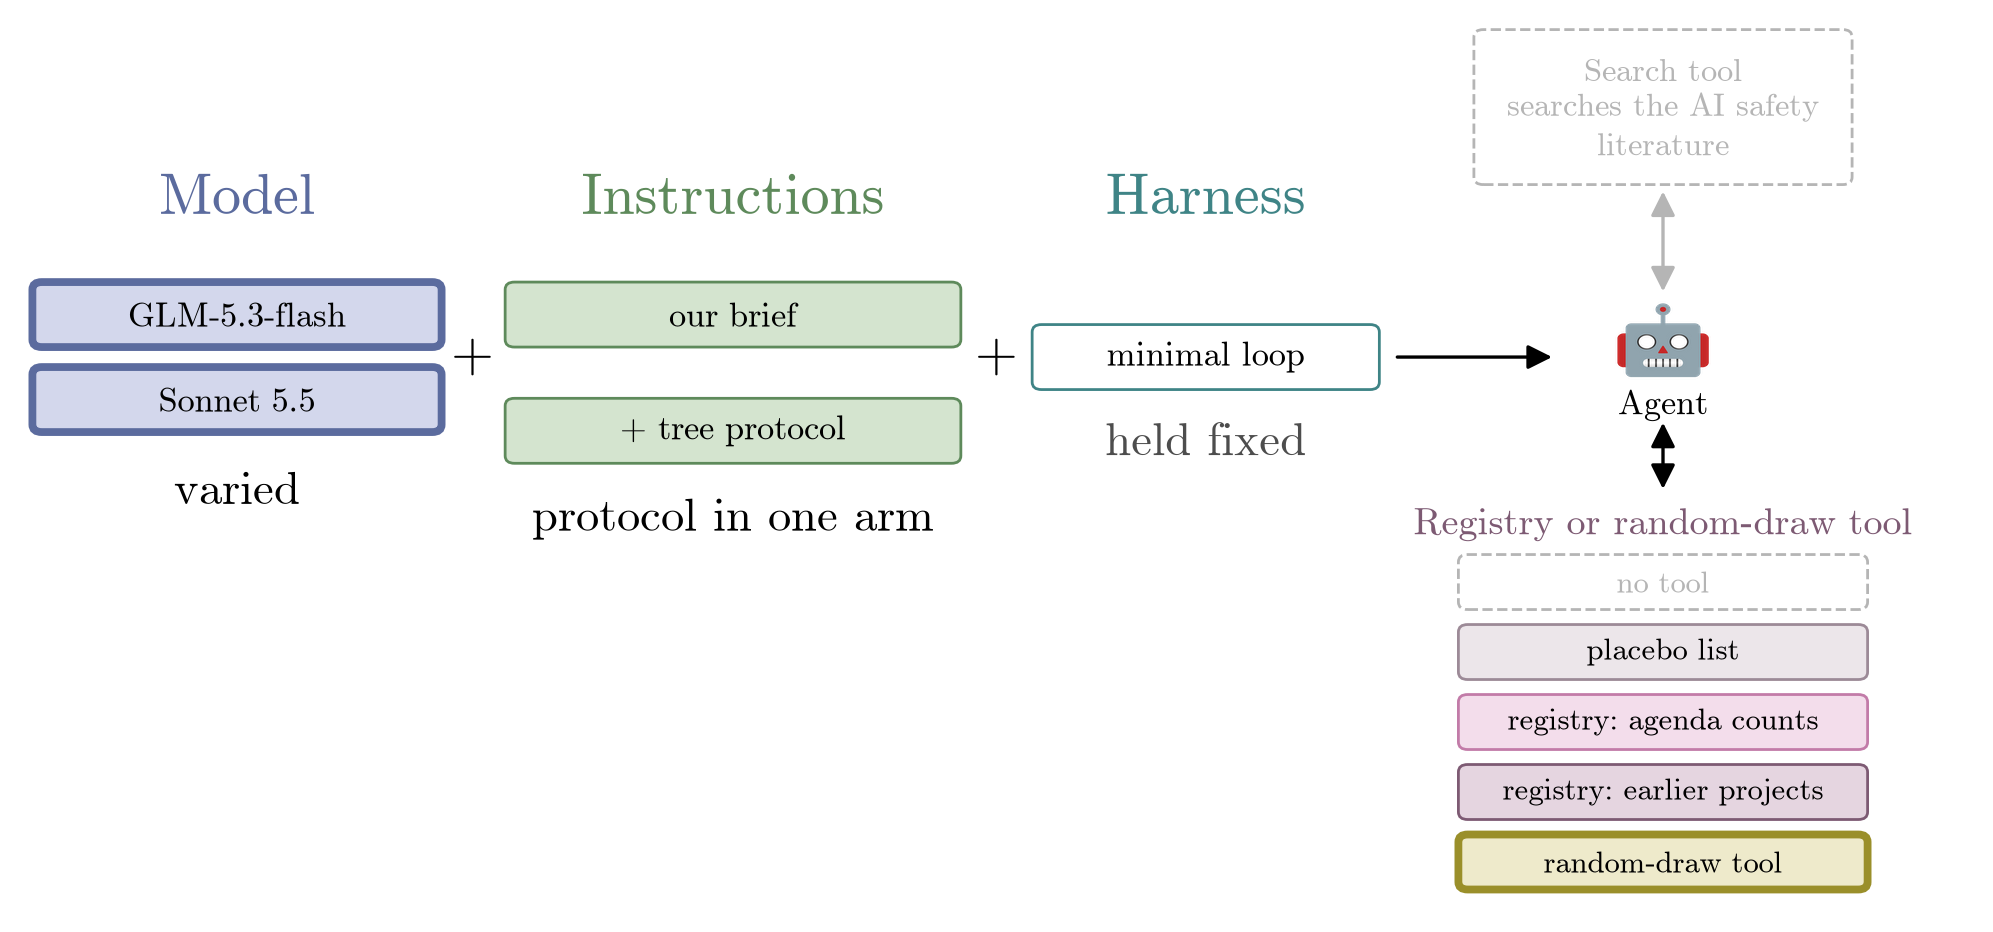
\includegraphics[keepaspectratio,alt={The setup for Figure A15, drawn as Figure 1: the simple setup with no registry or one of three, or with the tree protocol and the random-draw tool. Claude Sonnet 5.5 repeated only the tree test. The random-draw tool is bold because it contains randomness; the protocol's text does not.}]{figures/fig-A-setup-int.png}}
\caption{The setup for Figure A15, drawn as Figure 1: the simple setup
with no registry or one of three, or with the tree protocol and the
random-draw tool. Claude Sonnet 5.5 repeated only the tree test. The
random-draw tool is bold because it contains randomness; the protocol's
text does not.}\label{fig:A14}
\end{figure}

\begin{figure}
\centering
\pandocbounded{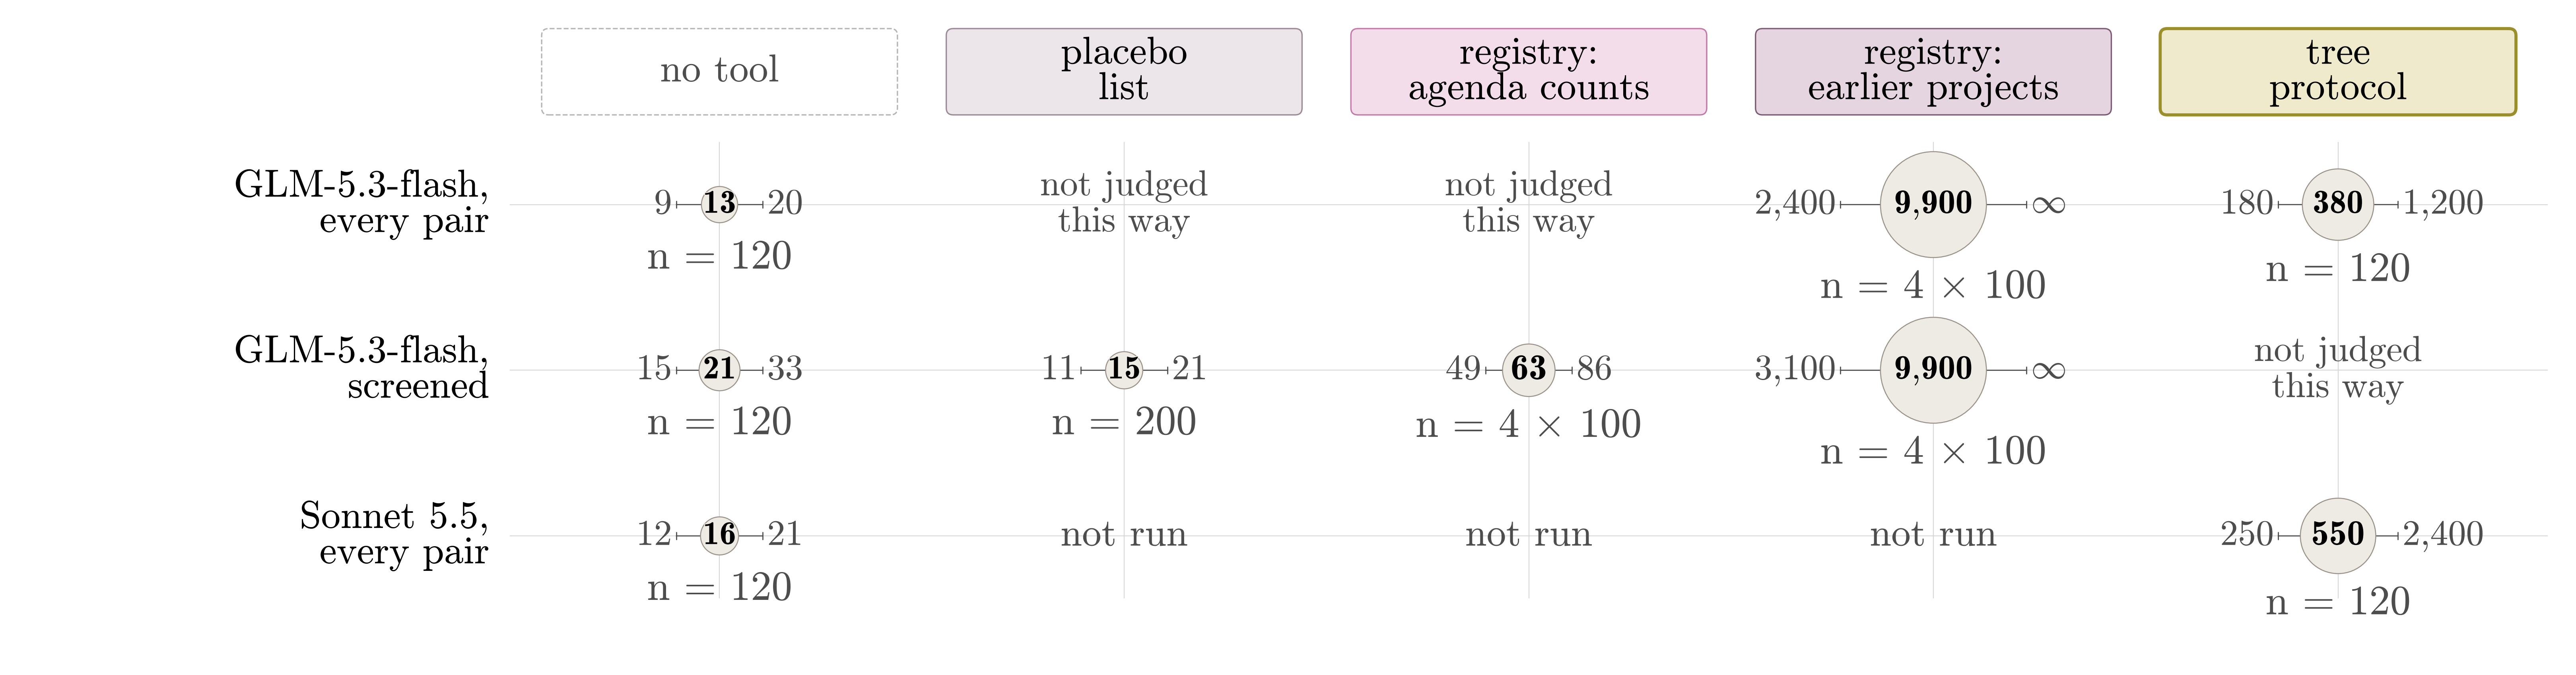
\includegraphics[keepaspectratio,alt={One column per intervention and one row per model and judging rule, each circle an effective number of projects with the ends of its 95\% interval either side and n below. Every pair means the judge read all pairs; screened means pairs far apart by a small embedding model were counted as different without asking it, the rule we used for the registry's first stage. Registry agents chose in four populations of 100, so only pairs within a population count; placebo agents chose independently, 200 in all; the other cells are groups of 120. ``Not judged this way'' marks a cell judged only under the other rule, and ``not run'' an arm that model did not run.}]{figures/fig-A-interventions.png}}
\caption{One column per intervention and one row per model and judging
rule, each circle an effective number of projects with the ends of its
95\% interval either side and \(n\) below. Every pair means the judge
read all pairs; screened means pairs far apart by a small embedding
model were counted as different without asking it, the rule we used for
the registry's first stage. Registry agents chose in four populations of
100, so only pairs within a population count; placebo agents chose
independently, 200 in all; the other cells are groups of 120. ``Not
judged this way'' marks a cell judged only under the other rule, and
``not run'' an arm that model did not run.}\label{fig:A15}
\end{figure}

This was the registry's first stage. Its curves over 100 agents look
like Figure 8's. A registry of earlier projects left 2 duplicate pairs
among 19,800, so few duplicates that neither judging rule can put an
upper limit on the number. Agenda counts cut the share of duplicate
pairs by about three quarters, much less than listing the projects
themselves. All 1,000 agents checked the registry before choosing.

With the protocol, the 120 GLM-5.3-flash agents behave as if they had
about 380 projects to choose from, against 13 without it. Judging all
299 agents we ran with the protocol gave about 480 (300 to 850), so the
first 120 were typical. A repeat of the simple setup with Claude Sonnet
5.5 in place of GLM-5.3-flash spread just as far, from about 16 projects
to about 550. Two checks that use no duplicate judge agree in direction:
the protocol tripled the number of agendas agents spread over, and moved
picks apart in a small text-embedding model's space.

\subsection{The GPT models under the pilot
brief}\label{the-gpt-models-under-the-pilot-brief}

\begin{figure}
\centering
\pandocbounded{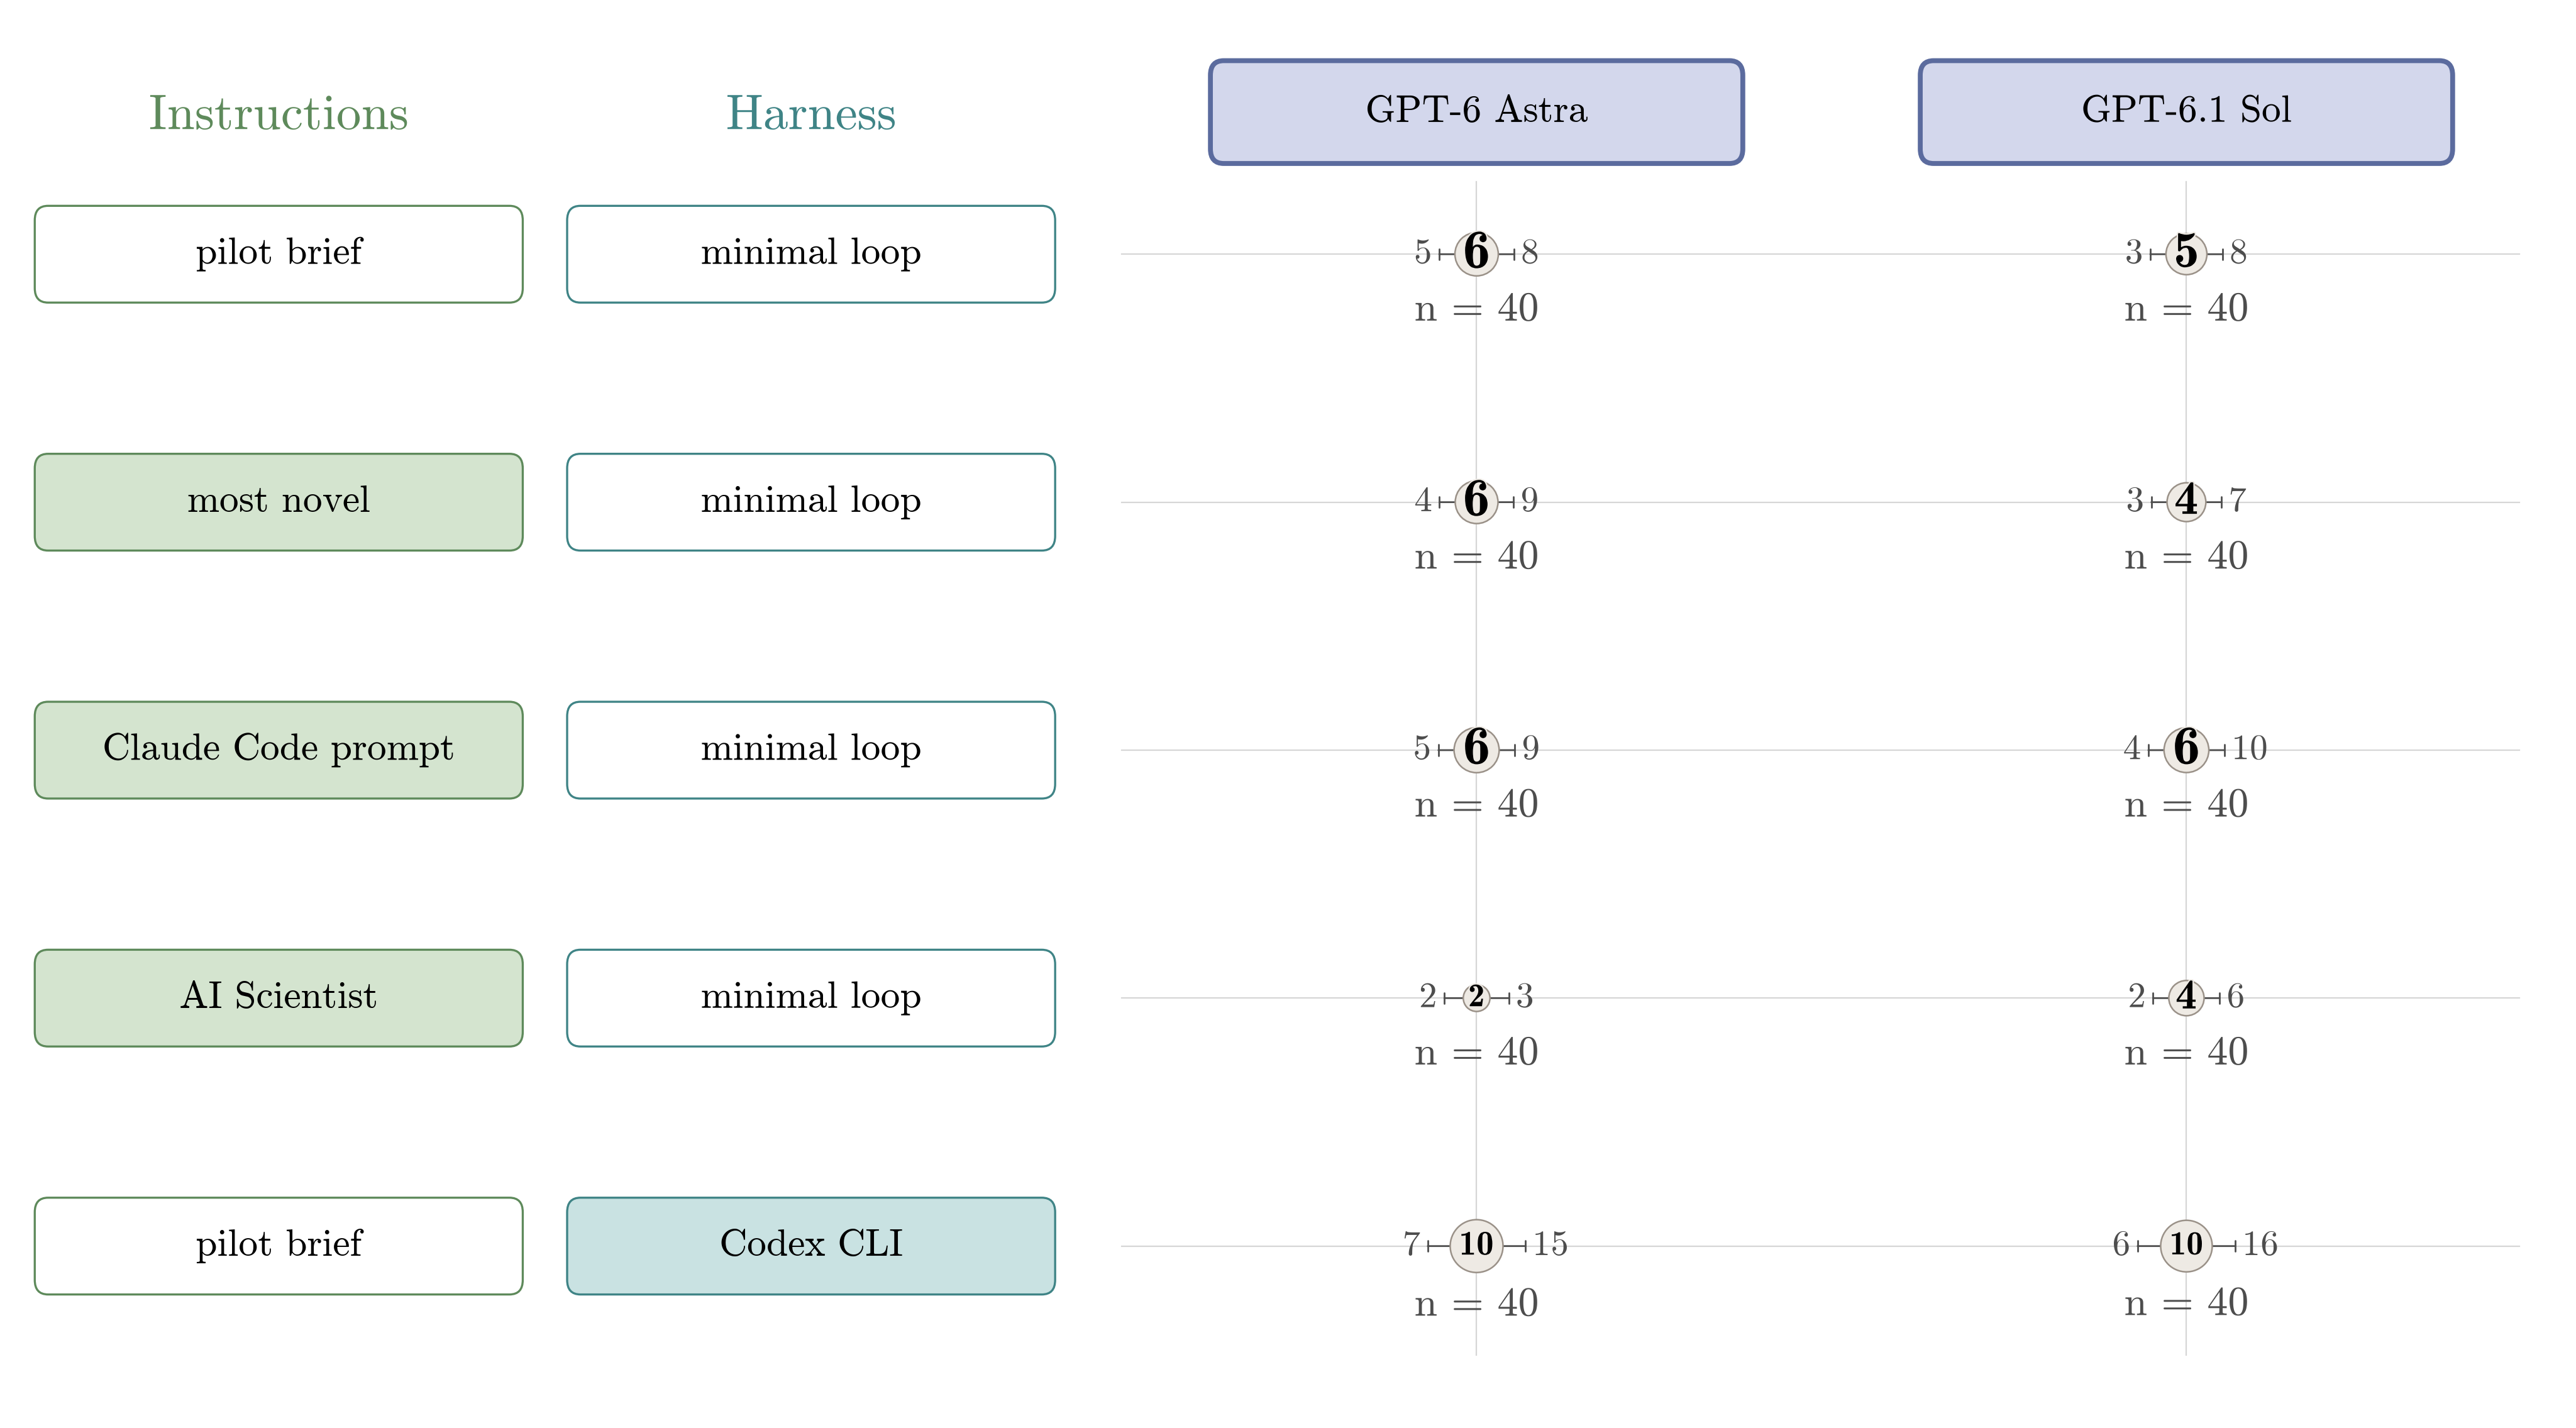
\includegraphics[keepaspectratio,alt={The two GPT models on the pilot version of the brief, one column per model and one row per setting: four instructions in the minimal loop, and our brief in Codex CLI. A shaded box is the setting that differs from our brief in the minimal loop. Each circle is an effective number of projects, with the ends of its 95\% interval either side and n below, with 40 agents per cell. The model headings are bold because every model samples its answer.}]{figures/fig-A2-gpt-setup.png}}
\caption{The two GPT models on the pilot version of the brief, one
column per model and one row per setting: four instructions in the
minimal loop, and our brief in Codex CLI. A shaded box is the setting
that differs from our brief in the minimal loop. Each circle is an
effective number of projects, with the ends of its 95\% interval either
side and \(n\) below, with 40 agents per cell. The model headings are
bold because every model samples its answer.}\label{fig:A16}
\end{figure}

The novelty sentence did nothing for the GPT models, and AI Scientist's
prompt narrowed them, because most GPT agents already propose one theme,
how an agent's stored memory can make untrusted claims look trusted, and
that prompt pushes them further toward it. Codex CLI roughly doubled
their spread.

\end{document}
